%!TEX root = ../template.tex
%%%%%%%%%%%%%%%%%%%%%%%%%%%%%%%%%%%%%%%%%%%%%%%%%%%%%%%%%%%%%%%%%%%%
%% chapter5.tex
%% NOVA thesis document file
%%
%% Chapter with lots of dummy text
%%%%%%%%%%%%%%%%%%%%%%%%%%%%%%%%%%%%%%%%%%%%%%%%%%%%%%%%%%%%%%%%%%%%

\typeout{NT FILE chapter5.tex}%

\chapter{Validation and Experimental Evaluation}\label{cha:validation}

In this chapter, we present the validation and experimental evaluation of the proposed solution. We start by discussing the evaluation criteria used to assess the quality of the present work, such as the used metrics to perform such measurements and the test benches employed. Then, we present the performance observations and results according to such criteria. 
Finally, we discuss the unobservability evaluation, and the formal validation of the proposed solution.

\section{Evaluation Criteria}\label{sec:evaluation_criteria}
To assess the quality of several aspects of the proposed solution, we defined a set of evaluation criteria as well as their importance to the overall system validation and evaluation. Tor is designed to protect users' privacy and anonymity, especially while web browsing, therefore is also important to evaluate the impact on performance. Tor already maintains a set of performance metrics and continuous evaluation, shared through Tor Metrics\footnote{\url{https://metrics.torproject.org/}}. Among several metrics and data collected by this project, we selected the most relevant and simple ones to compare our solution. Regarding performance, we used the standardized activity to evaluate the performance: \textit{download a file}. Tor Metrics uses 3 different file sizes to evaluate Tor: 50 KiB, 1 MiB and 5 MiB. Given this, we also tested our solution by downloading files of these sizes and compared the results regarding the throughput, the total time to download such files and the circuit round-trip latencies of circuits. 

Also, given the solution's goal to enhance Tor users' privacy and anonymity guarantees, we also considered the impact on the unobservability of the traffic. To evaluate the resistance of the solution, especially against attacks targeting website fingerprinting, such as the ones pointed out throughout this work as those carried by our adversaries, we conducted fingerprinting resistance tests. This tests allowed for a better understanding of the impact of the proposed solution on the unobservability of the traffic, and therefore on the anonymity guarantees. 

Finally, a formal validation of the proposed system was performed to mathematically express its privacy guarantees, leveraging established theorems of Differential Privacy.

\subsection{Test Benches}\label{sec:testbenches}

To conduct the before-mentioned tests, we design a couple of test benches to enlarge the scope of validation and evaluation of the solution. The testing environment for all test benches was designed to approximate a real-world scenario as closely as possible and to facilitate the easy replication and deployment of the experiments and their corresponding results. This was achieved by deploying two types of Tor networks:
\paragraph{Local Simulated Network} This tests bench focused on validating the solutions' extension of Tor, by simulating a minimal Tor network, with 4 relays (directory authority, 2 non-exit relays and 1 exit relay) and Tor client on a Docker Composed system on a single machine. Although this scenario does not replicate the exact conditions of a live Tor network, it served as a crucial preliminary stage for establishing and validating the deployment process of a private, minimal Tor network and for verifying the fundamental functionality of our proposed extensions. This test bench was performed on a single 2 vCores OVH\footnote{\url{https://www.ovhcloud.com/pt/}} Virtual Private Server (VPS) with 4 GB of RAM, configured with Ubuntu 24.10.
\paragraph{Distributed Network} This test bench aimed to evaluate our solution in a more realistic scenario, by emulating a small private distributed Tor network, with 4 relays and a Tor client, each deployed on a separate OVH VPS using Docker Swarm. On the tests. This test bench allowed us to evaluate the performance and unobservability of our solution in a more realistic environment, with network latencies and conditions closer to those of the real Tor network. This test bench was performed using 5 OVH VPSs, each with 2 vCores and 4 GB of RAM, configured with Ubuntu 24.10. These machines were dispersed through France, Germany, Poland and the United Kingdom.

\subsection{Experimental Observations}\label{sec:experimental_observations}

Our solution produced results for both performance and unobservability evaluations. The performance observations were performed using the \texttt{curl} command to download files of different sizes. The files were generated by a simple \textit{Python} web server hosted by our private network as a container, present in the directory authority machine, in case of the distributed test bench. The used command was:

\begin{lstlisting}[language=bash]
  $  curl --socks5 <tor_proxy> -H 'Cache-Control: no-cache' \
        -w 'Code: %{response_code}\n
           Time to first byte: %{time_starttransfer}s\n
           Total time: %{time_total}s\n
           Download speed: %{speed_download} bytes/sec\n' \
        -o /dev/null \
        <file_server_ip>:<file_server_port>/bytes/<file_size_in_bytes>
\end{lstlisting}

The \texttt{`socks5'} flag is required to route the traffic through the Tor network, therefore the \texttt{<tor\_proxy>} must be a tor client node. As mentioned before in~\autoref{subsec:deployment_for_validation_and_testing}, we recommend this request to be performed in the client node's machine and to assign the value \textit{`127.0.0.1:9000'} to \texttt{<tor\_proxy>}. The \texttt{file\_server\_ip} and \texttt{file\_server\_port} refer to the web server and, as the name suggests, the \texttt{file\_size\_in\_bytes} refers to the size of the file to be downloaded, in bytes. The used sizes were 51 200 bytes, 1 048 576 bytes 5 242 880 bytes, respectively the files used by Tor Metrics. The \texttt{-H 'Cache-Control: no-cache'} flag is used to prevent caching of the file, ensuring that each download request retrieves the file from the server rather than a cached version. The \texttt{-w} flag is used to format the output of the command, displaying the HTTP response code, for debugging purposes, time to first byte, to capture the latency, total time taken for the download, and download speed in bytes per second, referred onwards as throughput.

To collect data for the unobservability evaluation, we used the previous work of~\citeauthor{MIRACE}\cite{MIRACE}, by capturing traffic using \texttt{tcpdump} to \textit{pcap} files and then using the captured traces to trains and evaluate machine learning models to simulate website fingerprinting attacks. 

\section{Performance Evaluation}\label{sec:performance_evaluation}

To evaluate the performance of our solution, we conducted a series of experiments to measure the impact of the implemented features alone and in combination. In this section, we present the performance evaluation results, focusing on each metric. Firstly, we address the throughput results, followed by the total time taken to download files of different sizes, and finally, we analyze the latency results and the effect of the PPC feature on false cells and TLS packets count. 

The experiments were performed with variable configurations for both features. The Packet Padding Cells feature was tested with different $\epsilon$ values, ranging from 0 to 5, with more collections between 0 and 1, variable onwards referred as $\epsilon_d$. On the other hand, the Schedulers feature was also tested with different $\epsilon$ values, also ranging from 0 to 5, with more collections between 0 and 1, variable onwards referred as $\epsilon_j$. Additionally, when individually testing the Schedulers, we used different mathematical distributions to generate jitter: \textit{Poisson} and \textit{Exponential}. We also tested both features together, with variable $\epsilon_d$ and $\epsilon_j$ values, using the \textit{Poisson} distribution for jitter generation, due to time limitations of this work. These results are represented by heatmaps, with each $\epsilon$ as an axis, as the heat as the value of the metric.

In addition, we also present some results regarding the number of Packet Padding Cells generated during the experiments, compared with the TLS packets and total cells.

As mentioned earlier, the Tor Metrics project provides a continuous evaluation of the Tor network, including performance metrics such as throughput, total time to download files, and latency. In this chapter, we present our results and compare to the most recent results on Tor Metrics. The project provides results for 6 types of sources, but we focus on those which do not include the Conflux network, represented as mean of all medians. Conflux is a traffic splitting feature that Tor leverages to improve performance but, considering that our tests were conducted in a controlled and minimal network of relay, this features had no effect and must not be considered for results comparison. 

All experiments were conducted in the environments described in~\autoref{sec:evaluation_criteria} and compared with control tests performed without the implemented features, for baseline performance measurement, and with the Tor Metrics measures at the time of writing. The values presented in the following sections were obtained by performing a download 100 times for each configuration and calculating the median, 10th and 90th percentiles.

\subsection{Throughput}
Throughput is the unit of measurement that represents the amount of data flowing throw a certain point in the network. In our case, the throughput of the network is retrieved by downloading a file and measuring the download speed, in bytes per second. This is an important metric to evaluate the performance of our solution, as it directly impacts the user experience when browsing the web.

Below we share the throughput results obtained from our experiments and according to the above-mentioned test benches. We present the results for the local simulated environment in~\autoref{fig:local_throughput} and the distributed environment in~\autoref{fig:dist_throughput}. Each contains the corresponding results for each feature alone and both features combined, with the median represented as a thick line, together with a shaded area representing the first and third quartiles.

\begin{figure}[htbp]
    \centering
    \begin{subcaptionbox}{Only Packet Padding Cells Feature}[0.45\textwidth]
        {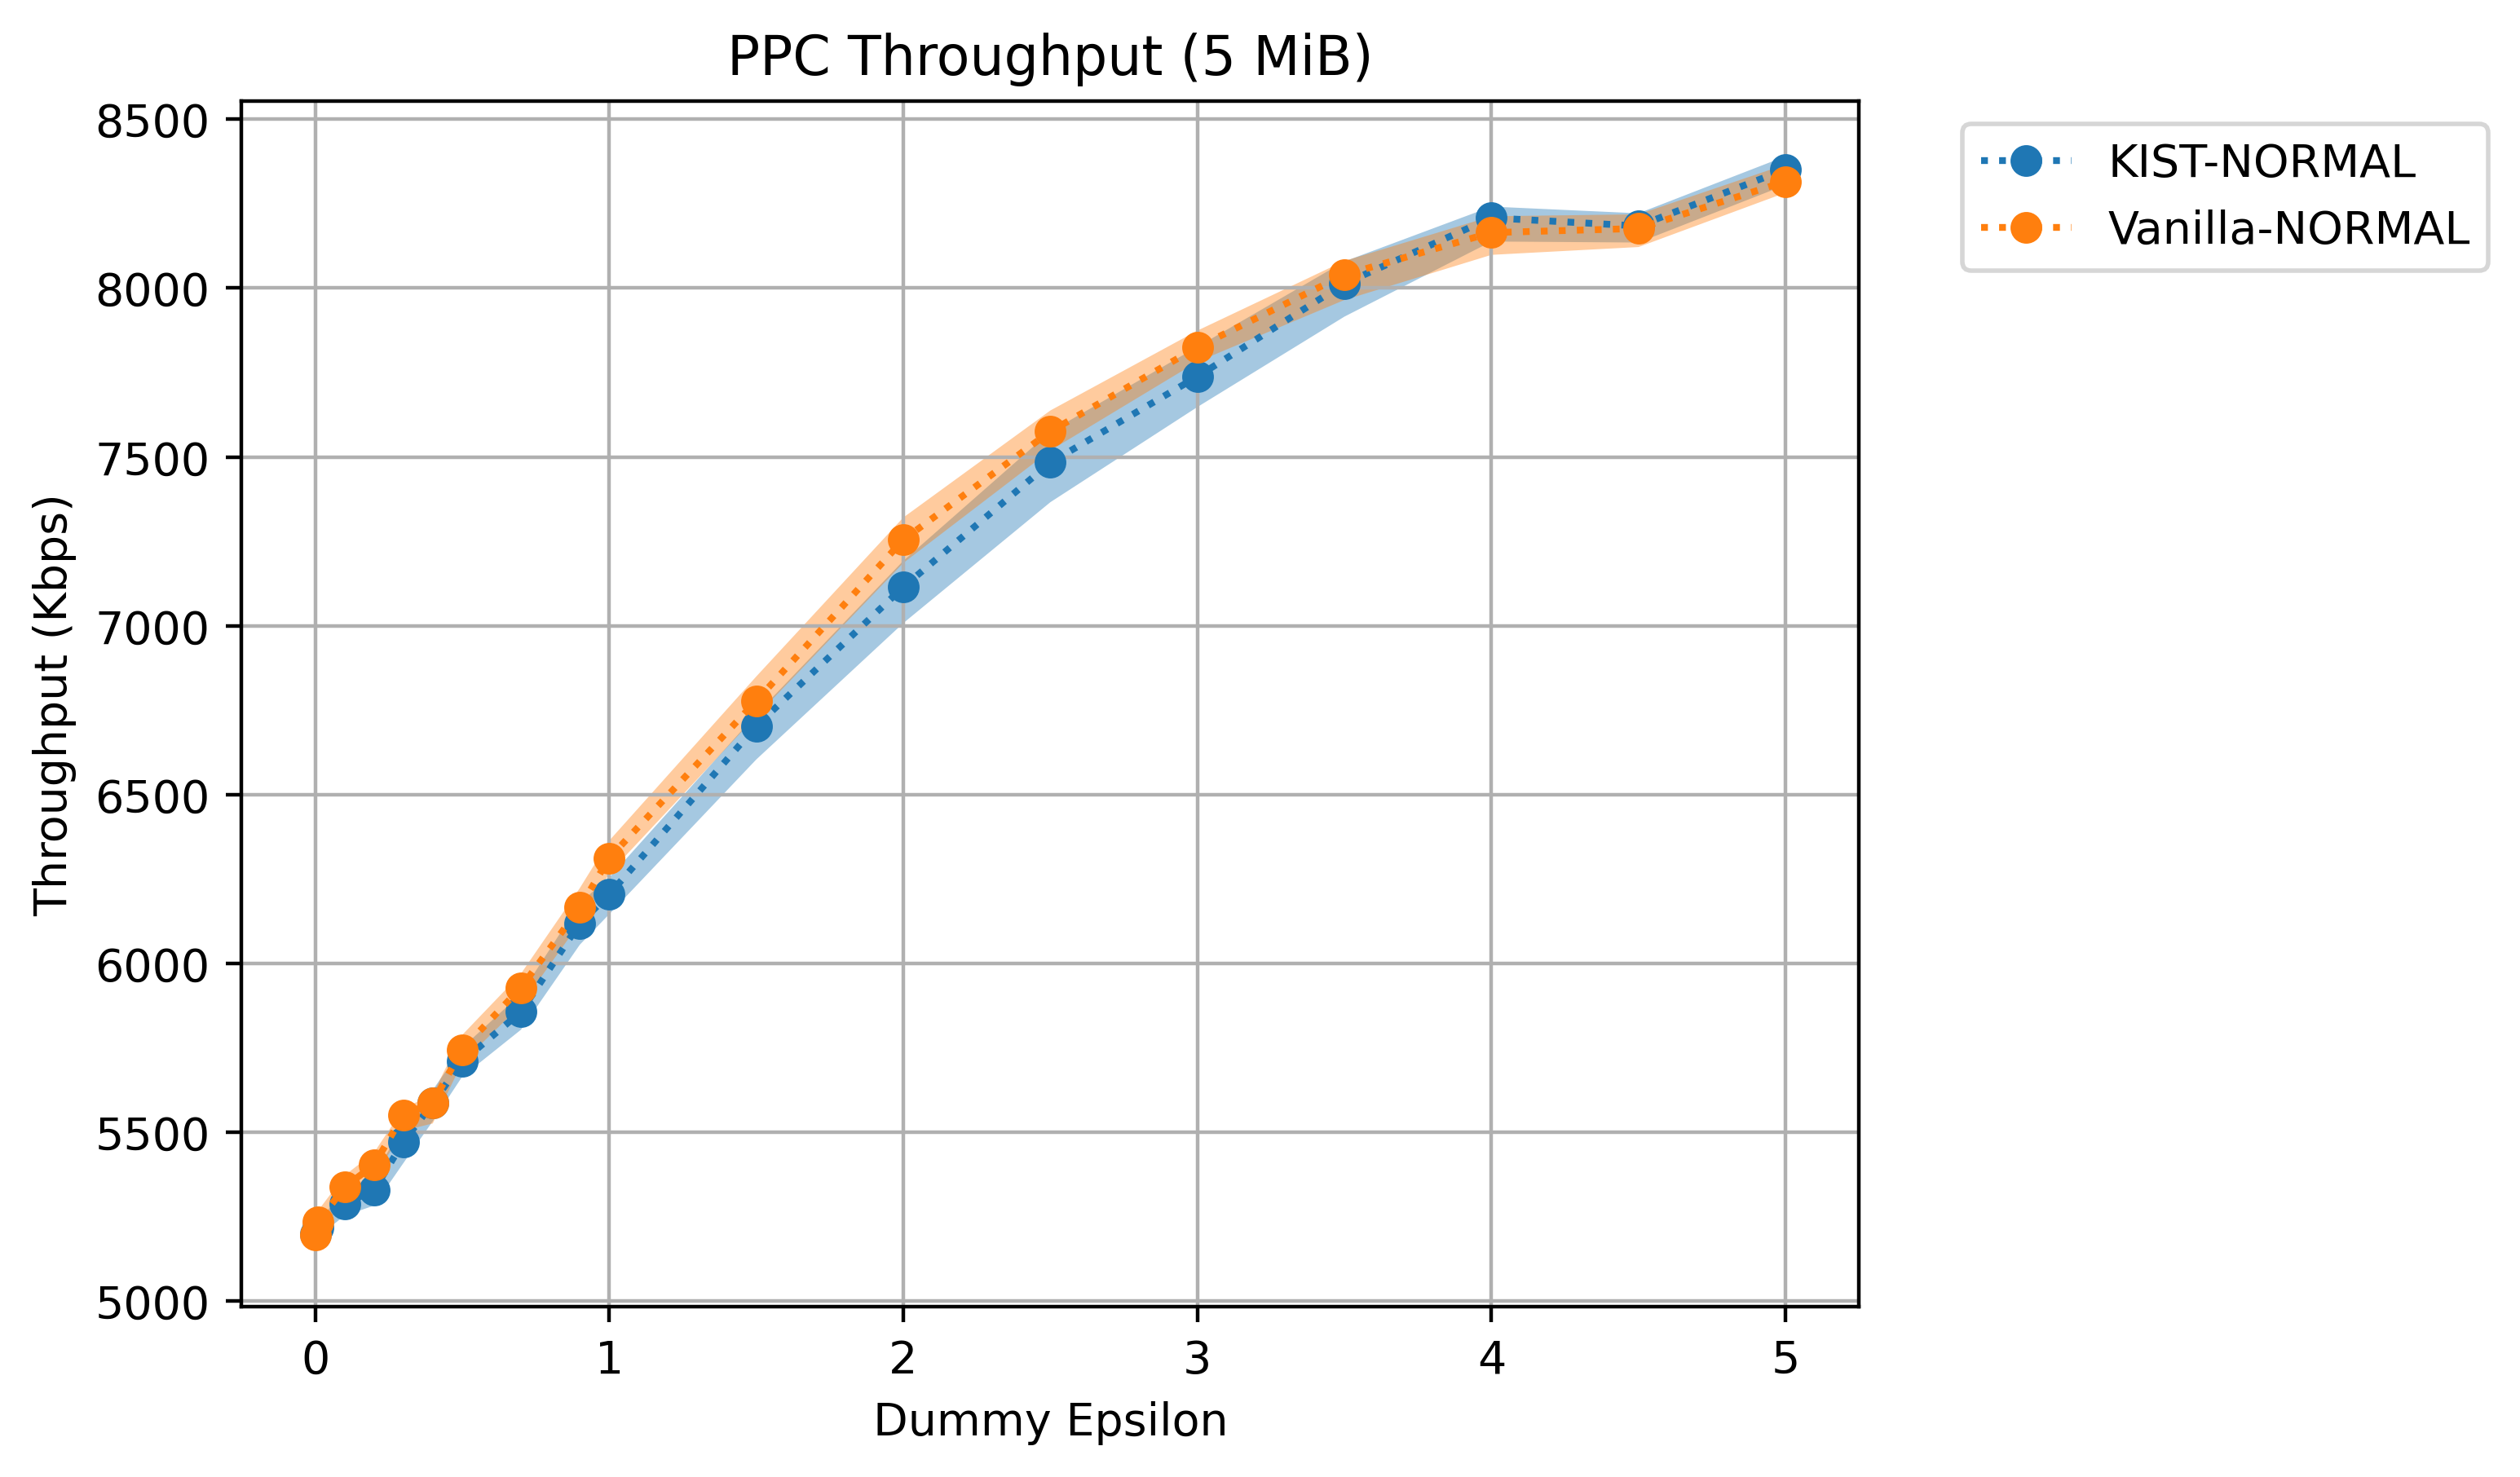
\includegraphics[width=\linewidth]{Chapters/Figures/Plots/local_throughput_50_PPC_5mib.png}\label{fig:local_ppc_throughput}}
    \end{subcaptionbox}
    \hfill
    \begin{subcaptionbox}{Only Jitter Injection Schedulers Feature\label{fig:local_jitter_throughput}}[0.45\textwidth]
        {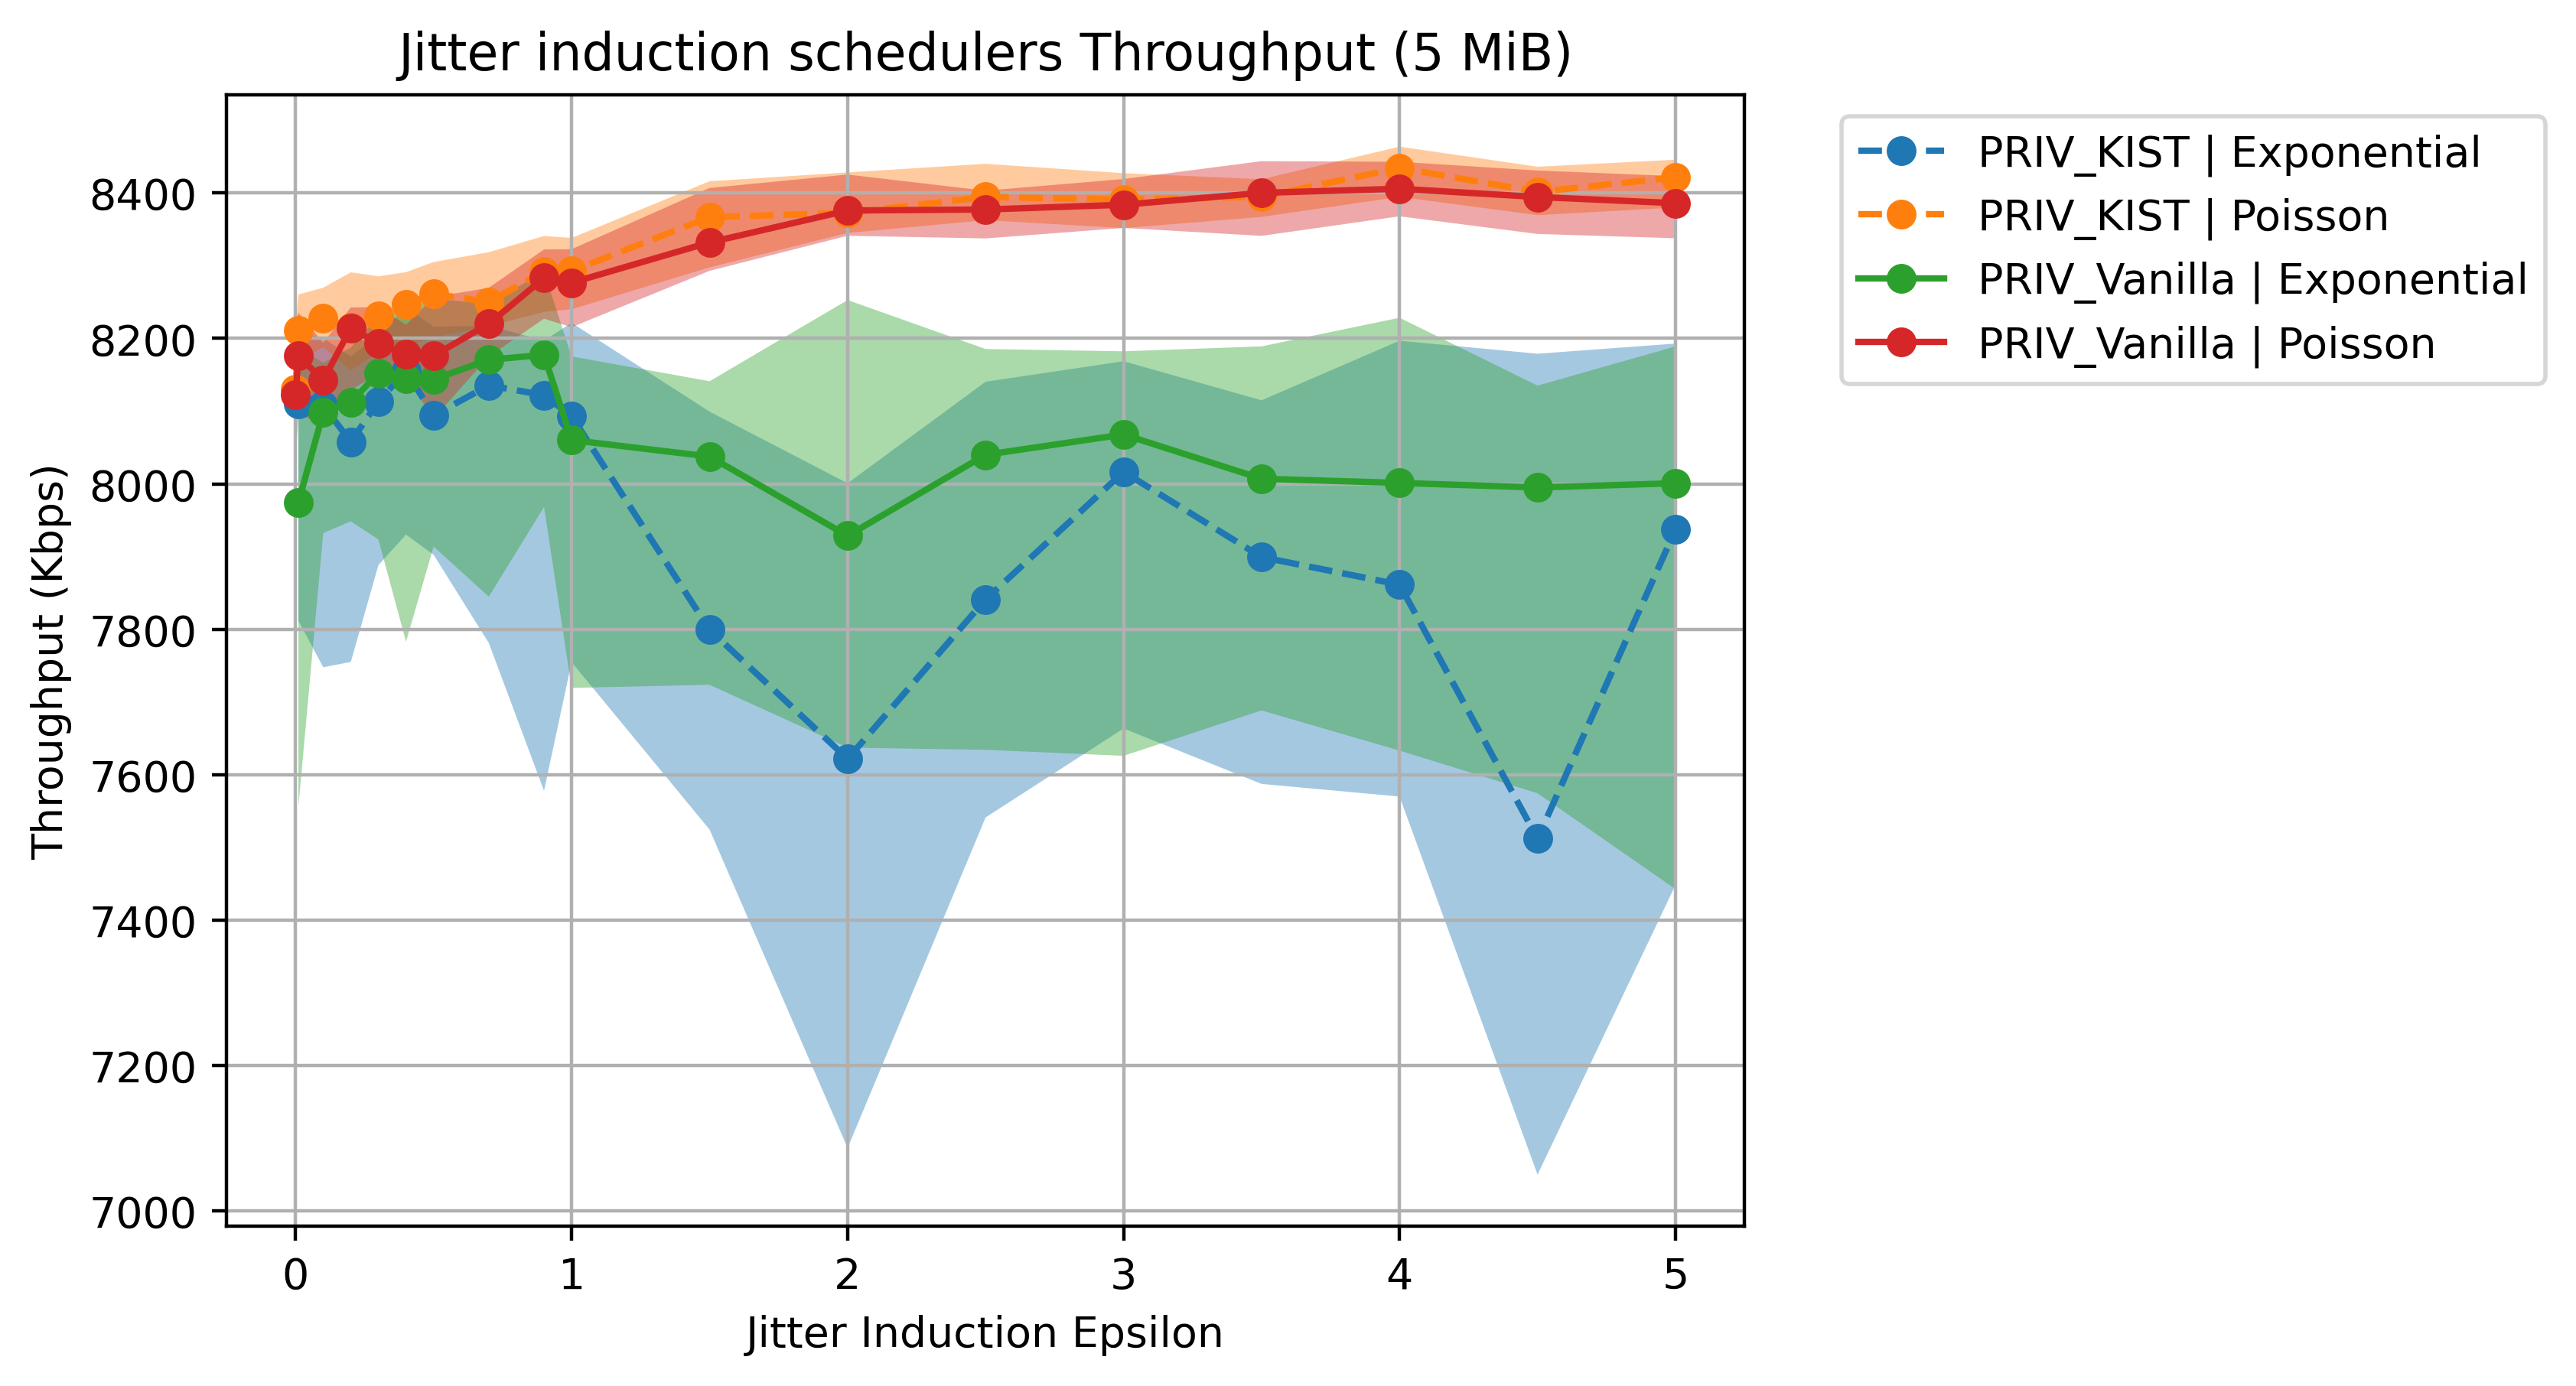
\includegraphics[width=\linewidth]{Chapters/Figures/Plots/local_throughput_50_jitter_5mib.png}}
    \end{subcaptionbox}
    \vfill
    \begin{subcaptionbox}{Both Features\label{fig:local_both_throughput}}[0.65\textwidth]
        {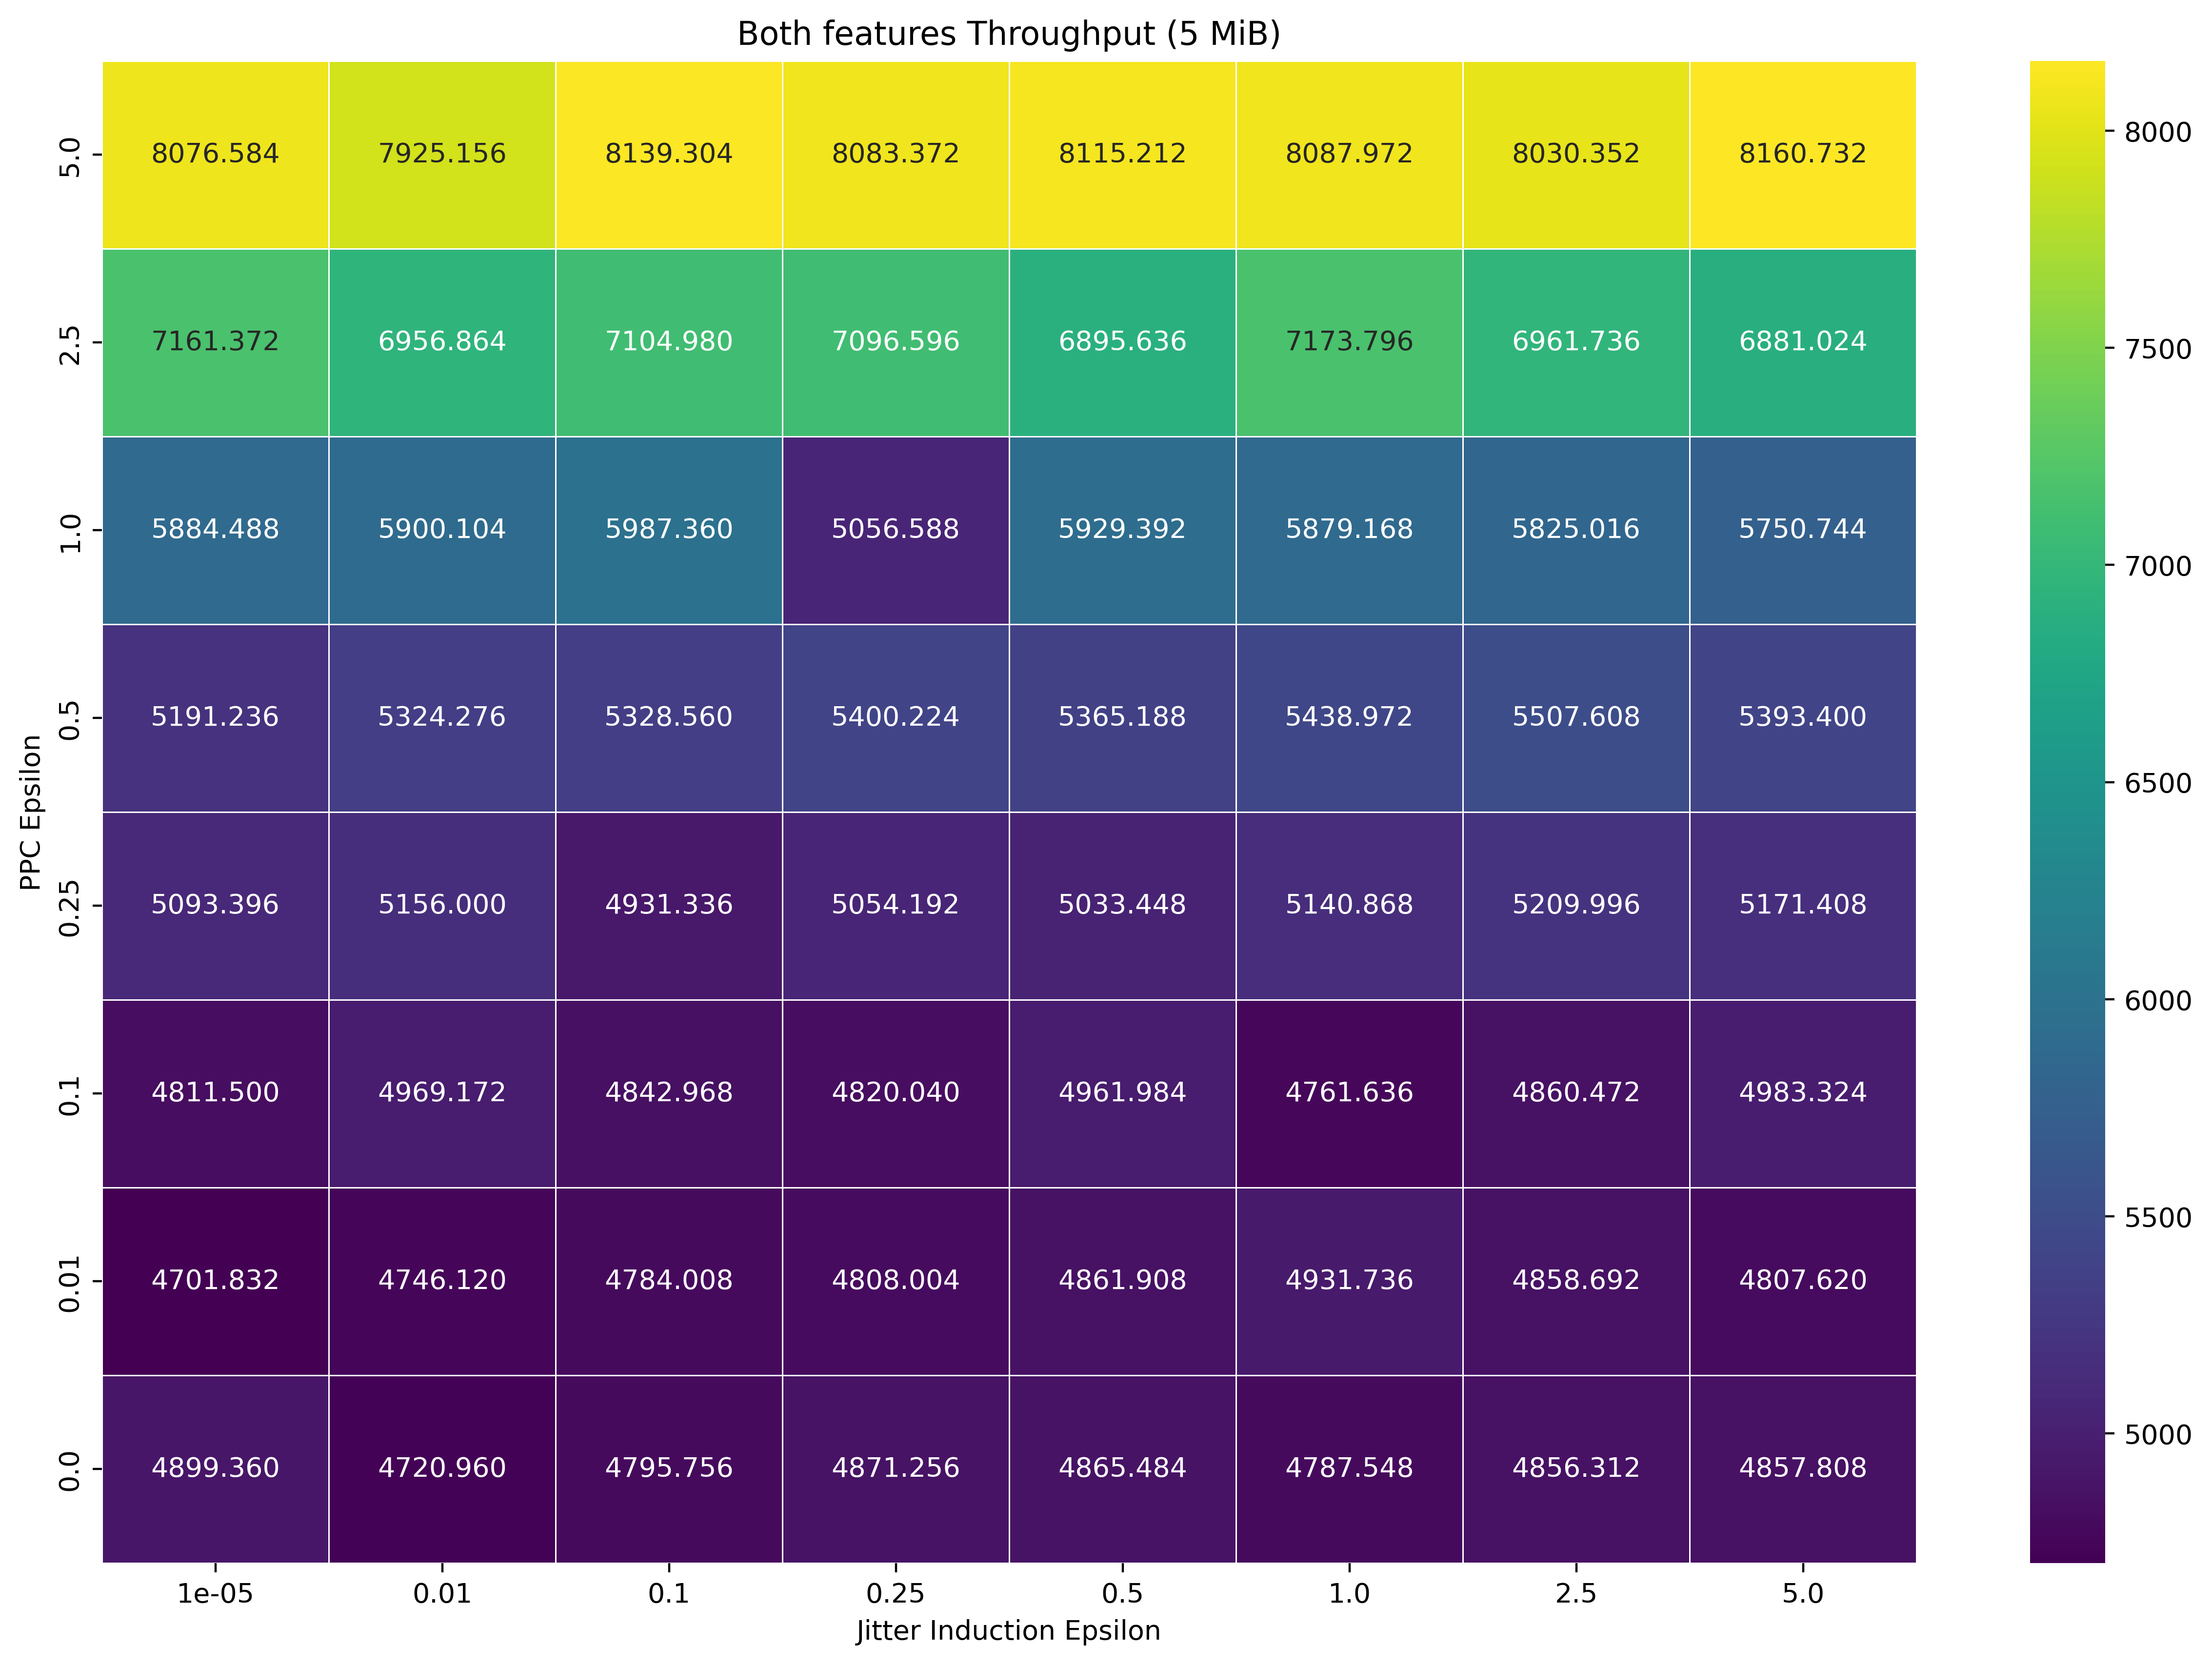
\includegraphics[width=\linewidth]{Chapters/Figures/Plots/local_throughput_50_heatmap_5mib.png}}
    \end{subcaptionbox}
    \caption{Throughput Results on Local Simulated Environment}\label{fig:local_throughput}
\end{figure}

\begin{figure}[htbp]
    \centering
    \caption{Throughput Results on Distributed Environment}\label{fig:dist_throughput}
    \begin{subcaptionbox}{Only Packet Padding Cells Feature\label{fig:dist_ppc_throughput}}[0.45\textwidth]
        {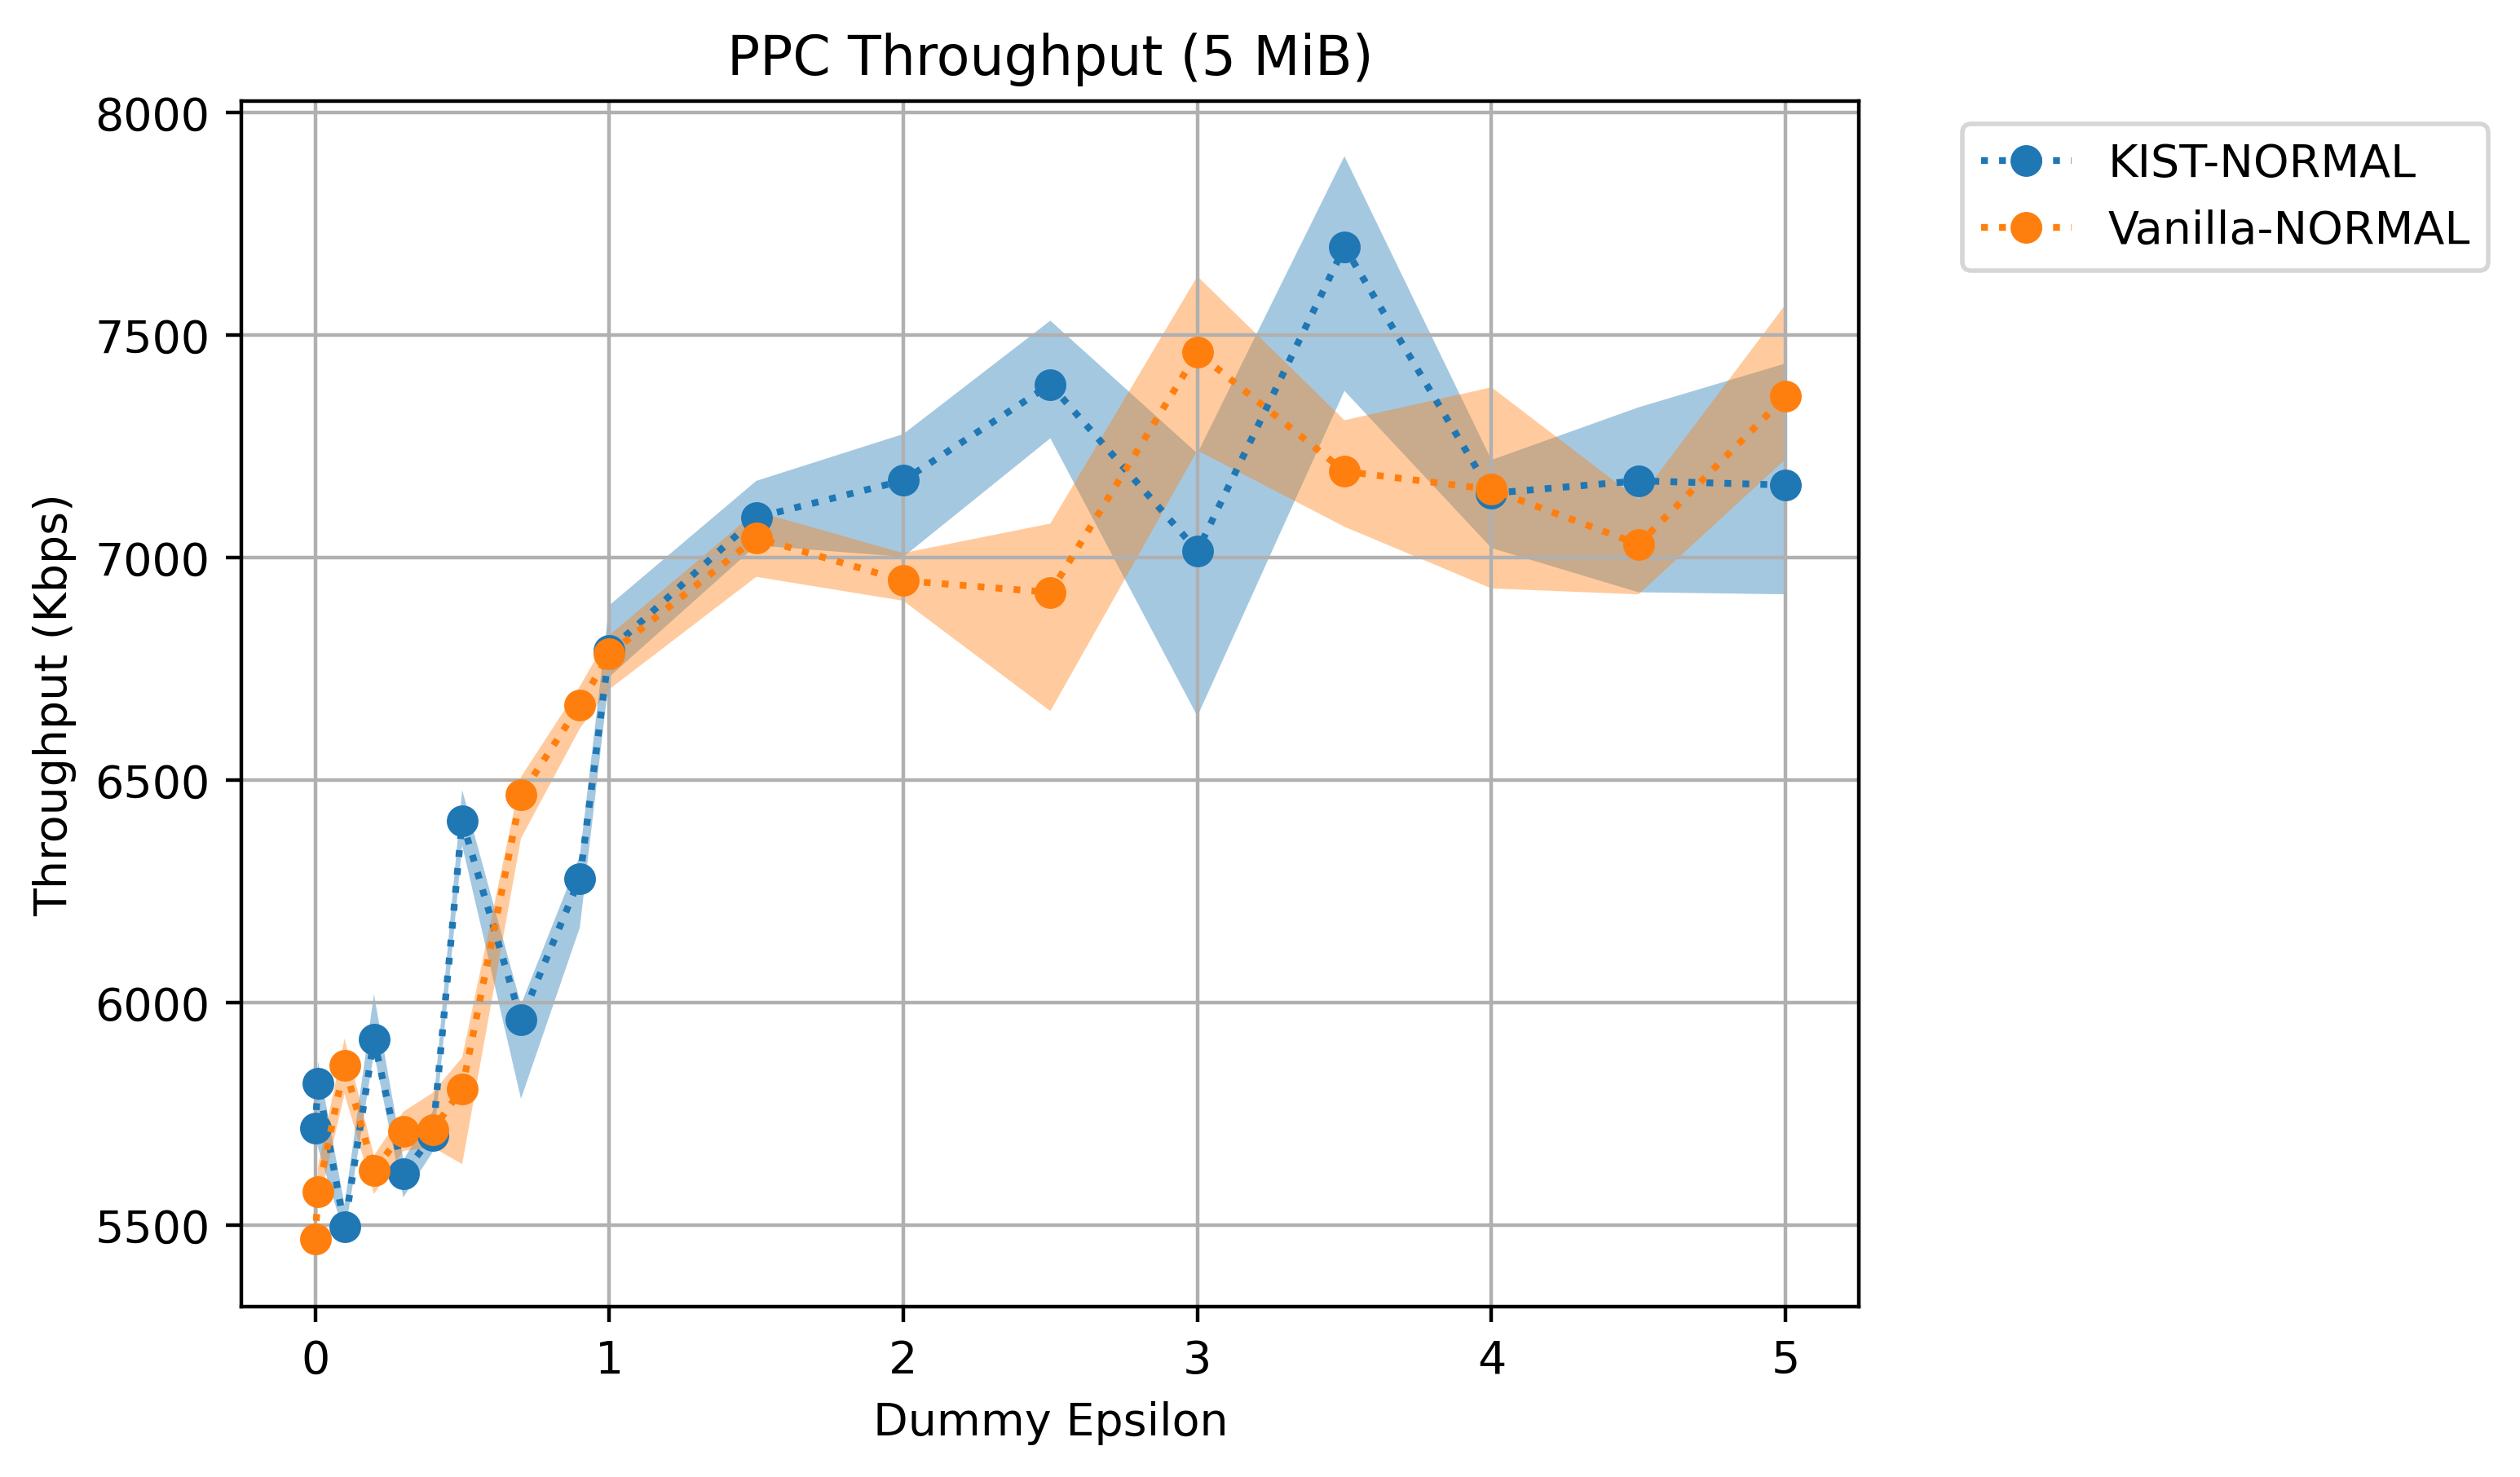
\includegraphics[width=\linewidth]{Chapters/Figures/Plots/dist_throughput_50_PPC_5mib.png}}
    \end{subcaptionbox}
    \hfill
    \begin{subcaptionbox}{Only Jitter Injection Schedulers Feature\label{fig:dist_jitter_throughput}}[0.45\textwidth]
        {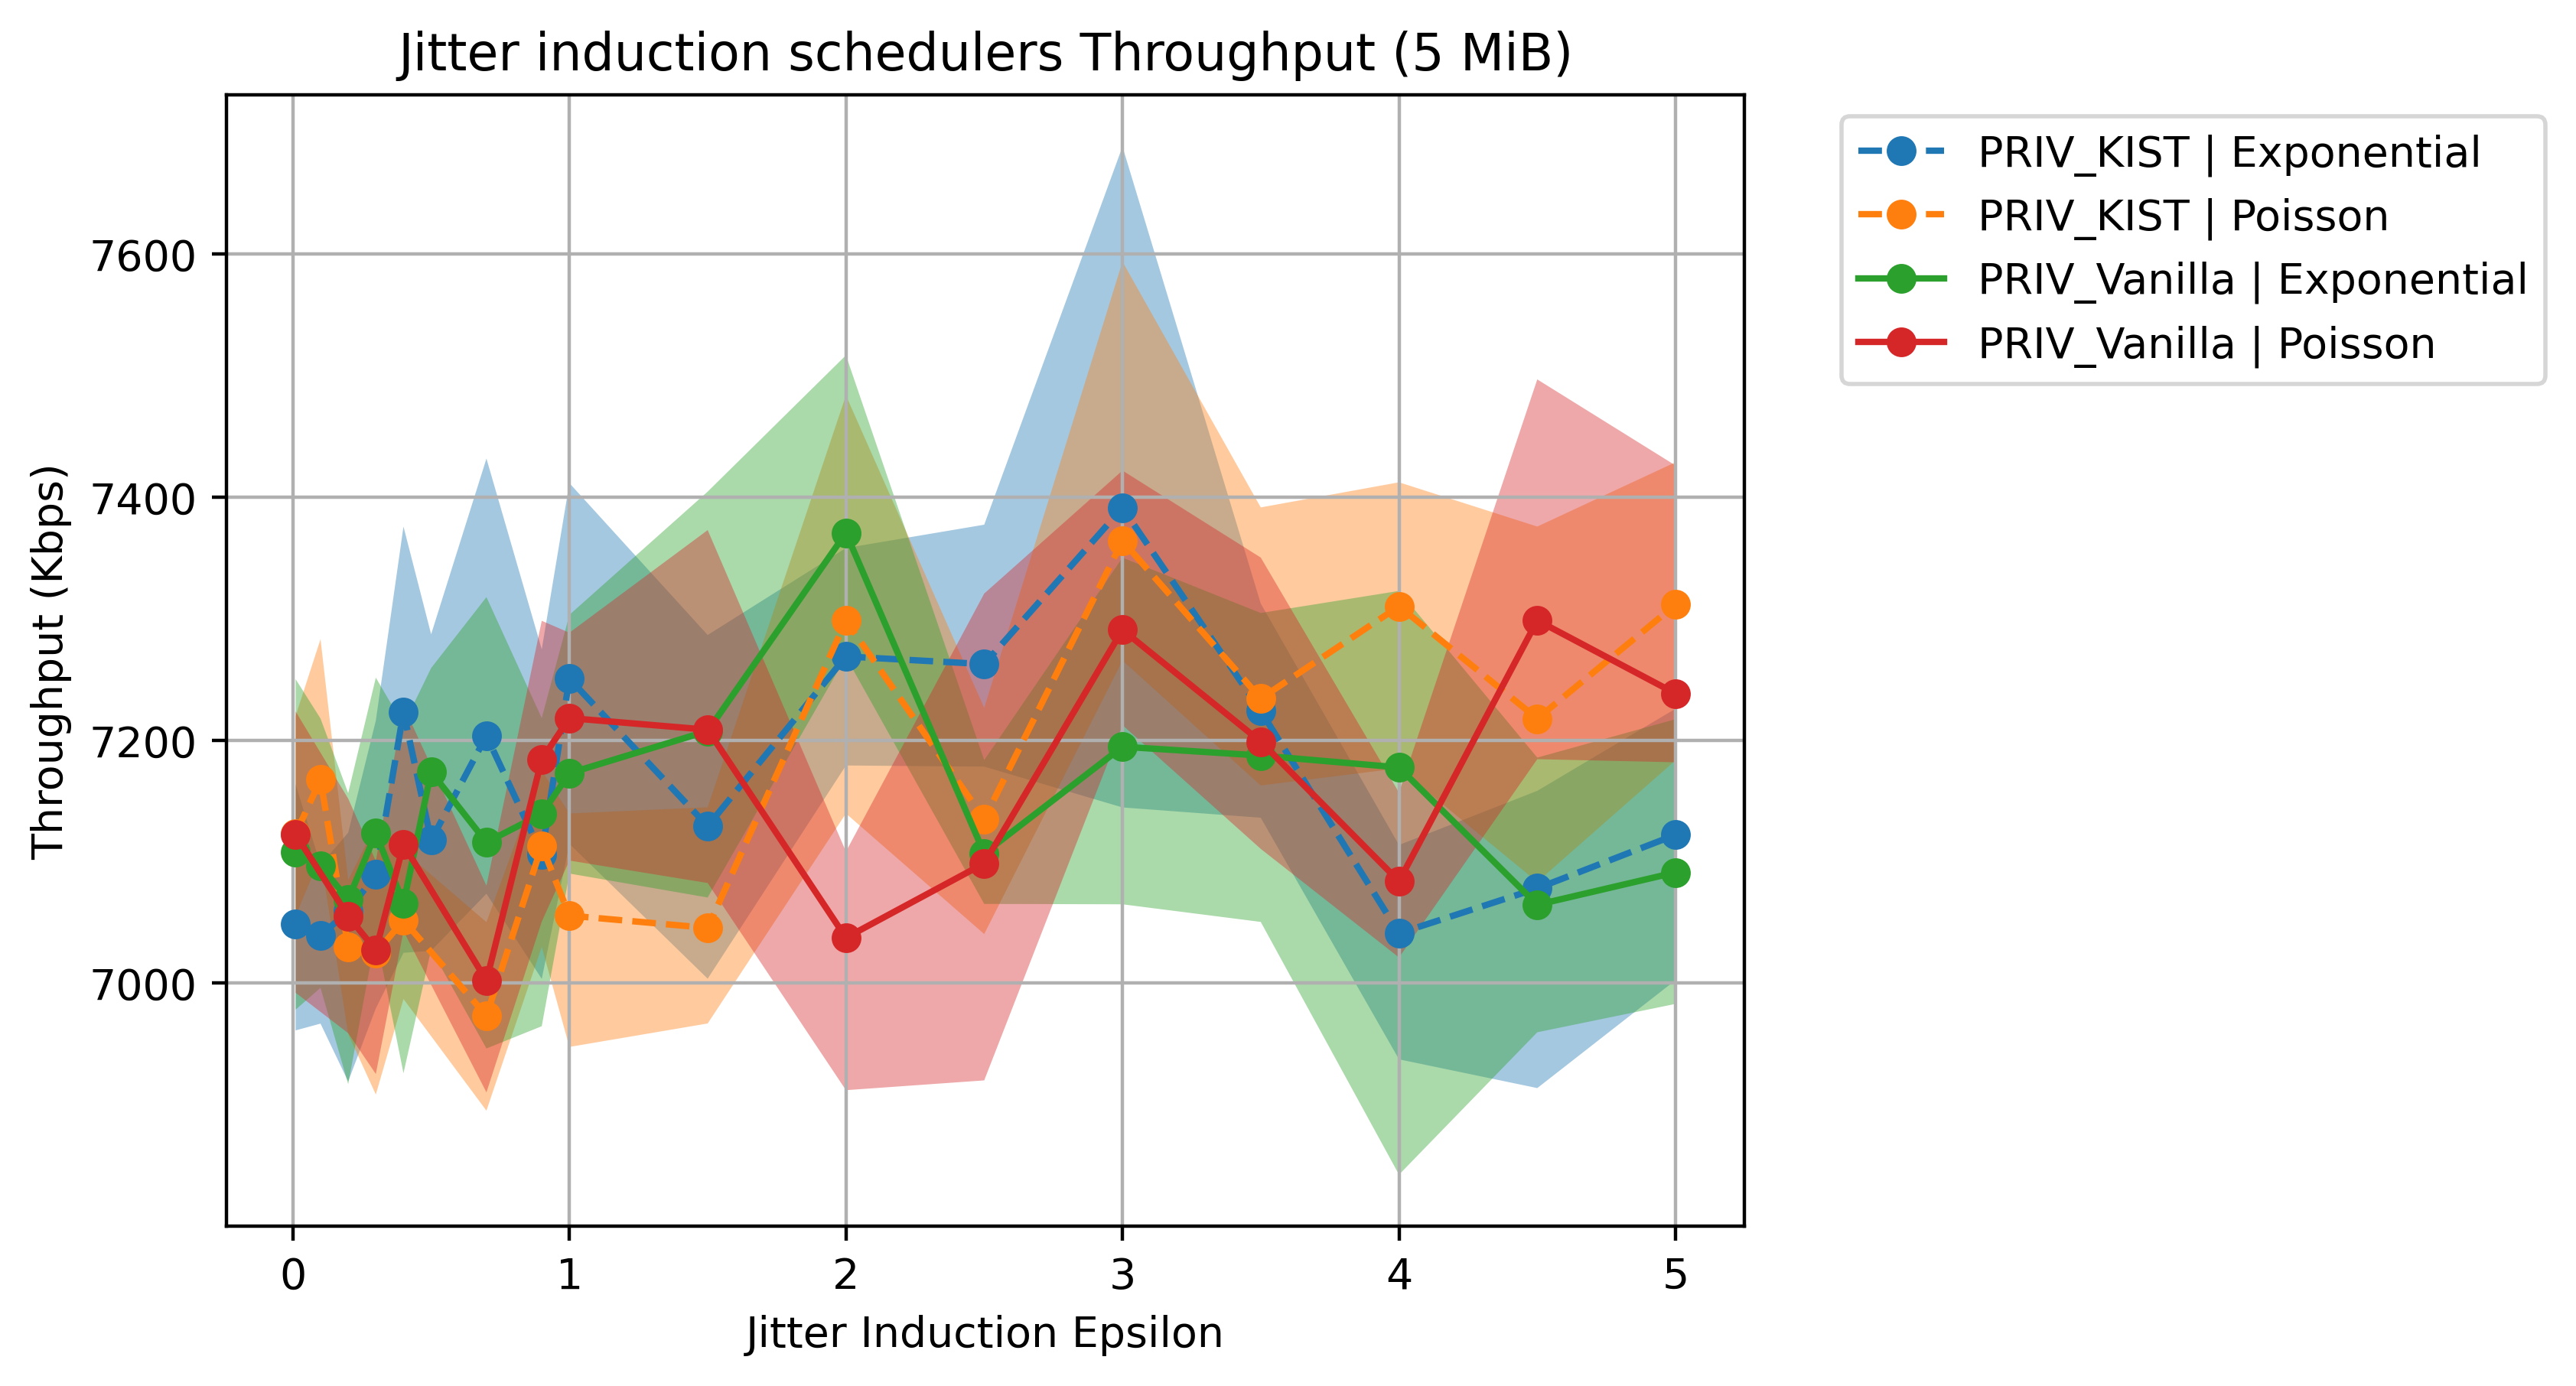
\includegraphics[width=\linewidth]{Chapters/Figures/Plots/dist_throughput_50_jitter_5mib.png}}
    \end{subcaptionbox}
    \vfill
    \begin{subcaptionbox}{Both Features\label{fig:dist_both_throughput}}[0.65\textwidth]
        {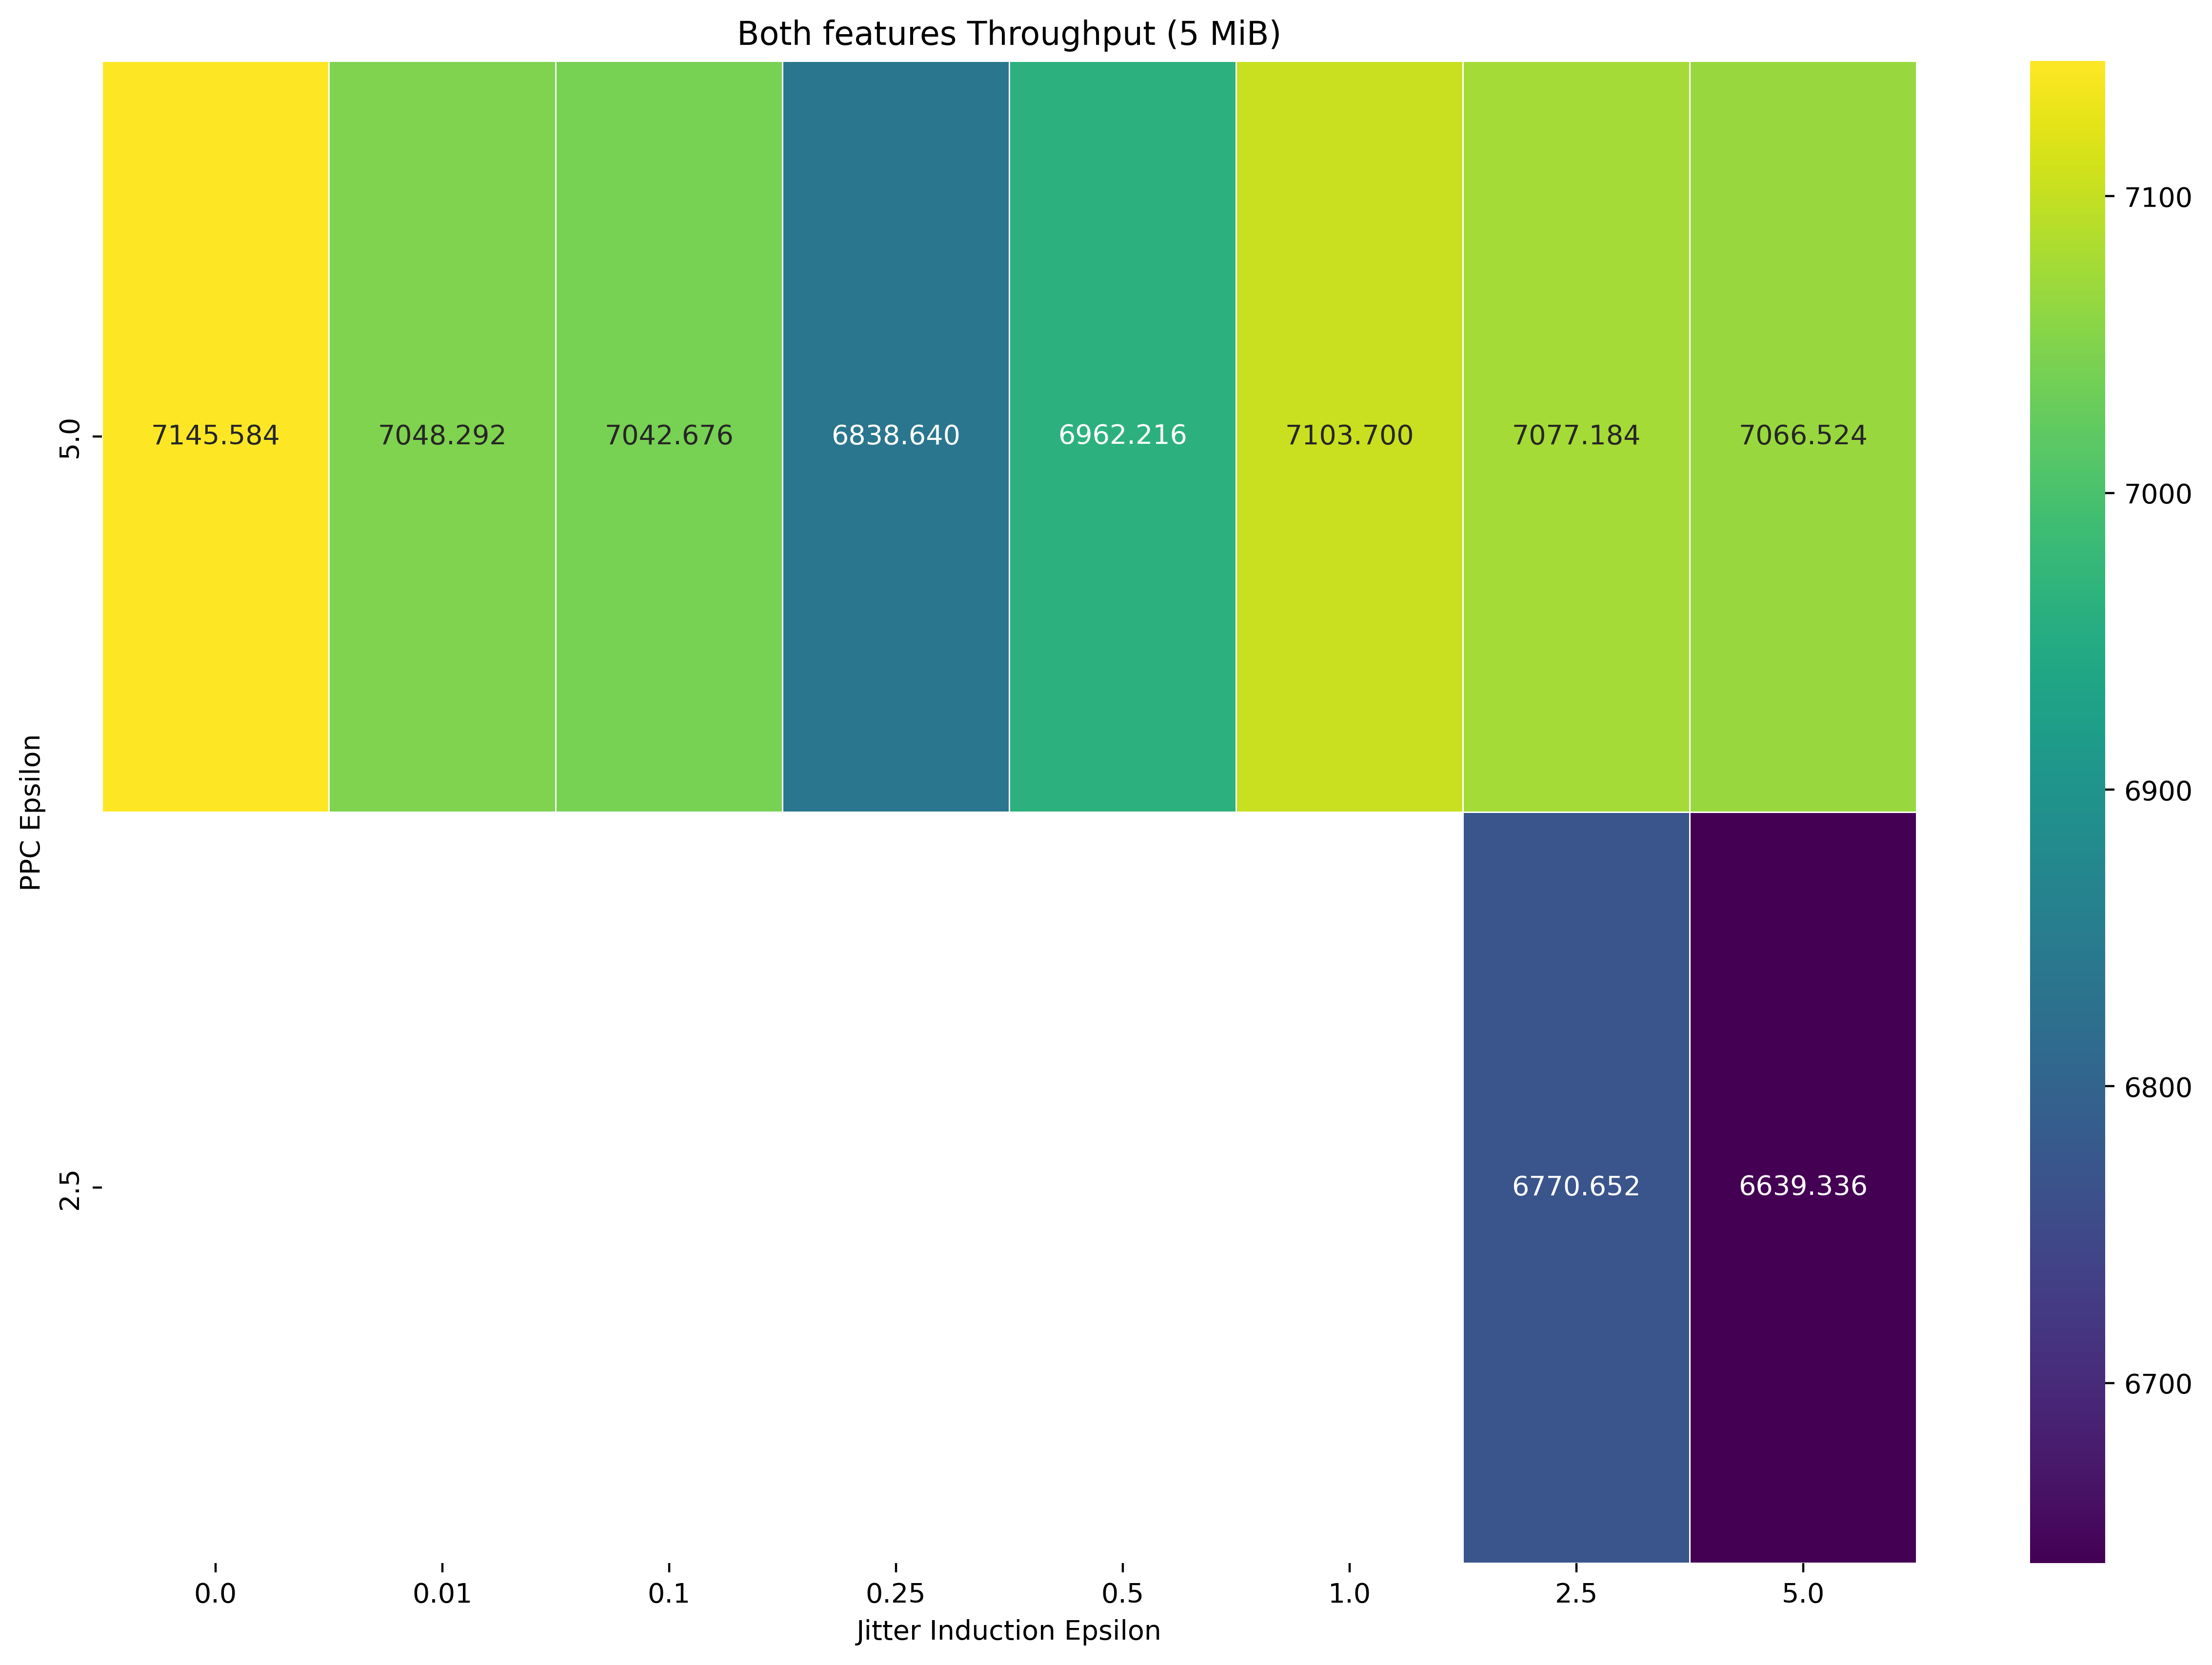
\includegraphics[width=\linewidth]{Chapters/Figures/Plots/dist_throughput_50_heatmap_5mib.png}}
    \end{subcaptionbox}
\end{figure}

As shown in~\autoref{fig:local_throughput} and~\autoref{fig:dist_throughput}, the PPC feature has a more significant impact on throughput than the Schedulers feature. 
This impact has greater impact as $\epsilon_{PPC}$ decrease, reaches a plateau when $\epsilon_{PPC}$ is greater than 4. The distributed test bench showed more unstable results, but the overall trend is similar. The Schedulers feature has a smaller impact on throughput, with a slight decrease for $\epsilon_{J}$ values closer to 0. A notable anomaly was observed in the local emulated test bench: for $\epsilon_{J}$ values greater than 1, the throughput results exhibited increased statistical variance and a slight degradation in performance when using the Exponential distribution. This suggests that at lower privacy levels (higher $\epsilon$), the scheduling delays introduced by this specific distribution may create contention or inefficiencies not present with other distributions.

In all experiments, all types schedulers behaved similarly.
For the experiments with both features enabled, the results emphasized the greater impact of the PPC feature on throughput. The heatmap clearly shows that the throughput only oscillate vertically, but remain consistent across different $\epsilon_{J}$ values.

As time of writing, Tor Metrics reports a median throughput value of 18 236 Mbps for files downloaded over the Tor network. Although, is important to note that these values are sampled from downloads of different files and only measure the throughput value between 4 MiB and 5 MiB of such files. In our case, we compare this value with the throughput values obtained from downloading files of 5 MiB.
%TODO: MUST TEST COMBINATIONS ON DISTRIBUTED TO GET BETTER ANALYSIS ON WORSE/BETTER TEST BENCH AND CONFIGURATION

\begin{table}[htbp]
    \centering
    \begin{tabular}{|c|c|c|}
    \hline
    \textbf{Configuration} & \textbf{Local} & \textbf{Distributed} \\
    \hline
    Tor Metrics& \multicolumn{2}{c|}{11 587} \\ 
    \hline
    \multirow{2}{*}{Control} & 8 240 & 7 045\\ 
    & 8 235 & 7 298\\
    \hline
    Only PPC & 5 197 – 8 351 & 5 469 – 7 699\\
    \hline
    Only Jitter & 7 512 – 8 435 & 6 973 – 7 391\\
    \hline
    PPC \& Jitter & 4 721 – 8 161 & 6 639 – 7 146\\
    \hline
    \end{tabular}
    \caption{Throughput Results Summary (Mbps)}\label{tab:throughput_summary}
\end{table}

\FloatBarrier
\subsection{Total Time}

Evaluating the total time necessary to download a file is also important to understand the effects of our solution on user experience and performance. Therefore, we present the total time results obtained from our experiments in~\autoref{fig:local_total_time} for the local simulated environment and~\autoref{fig:dist_total_time} for the distributed environment. We followed the Tor Metrics directives and also present the results as a thick line which represents the median value, together with a shaded area representing the first and third quartiles.

\begin{figure}[htbp]
    \centering
    \begin{subcaptionbox}{Only Packet Padding Cells Feature\label{fig:local_ppc_total_time}}[0.45\textwidth]
        {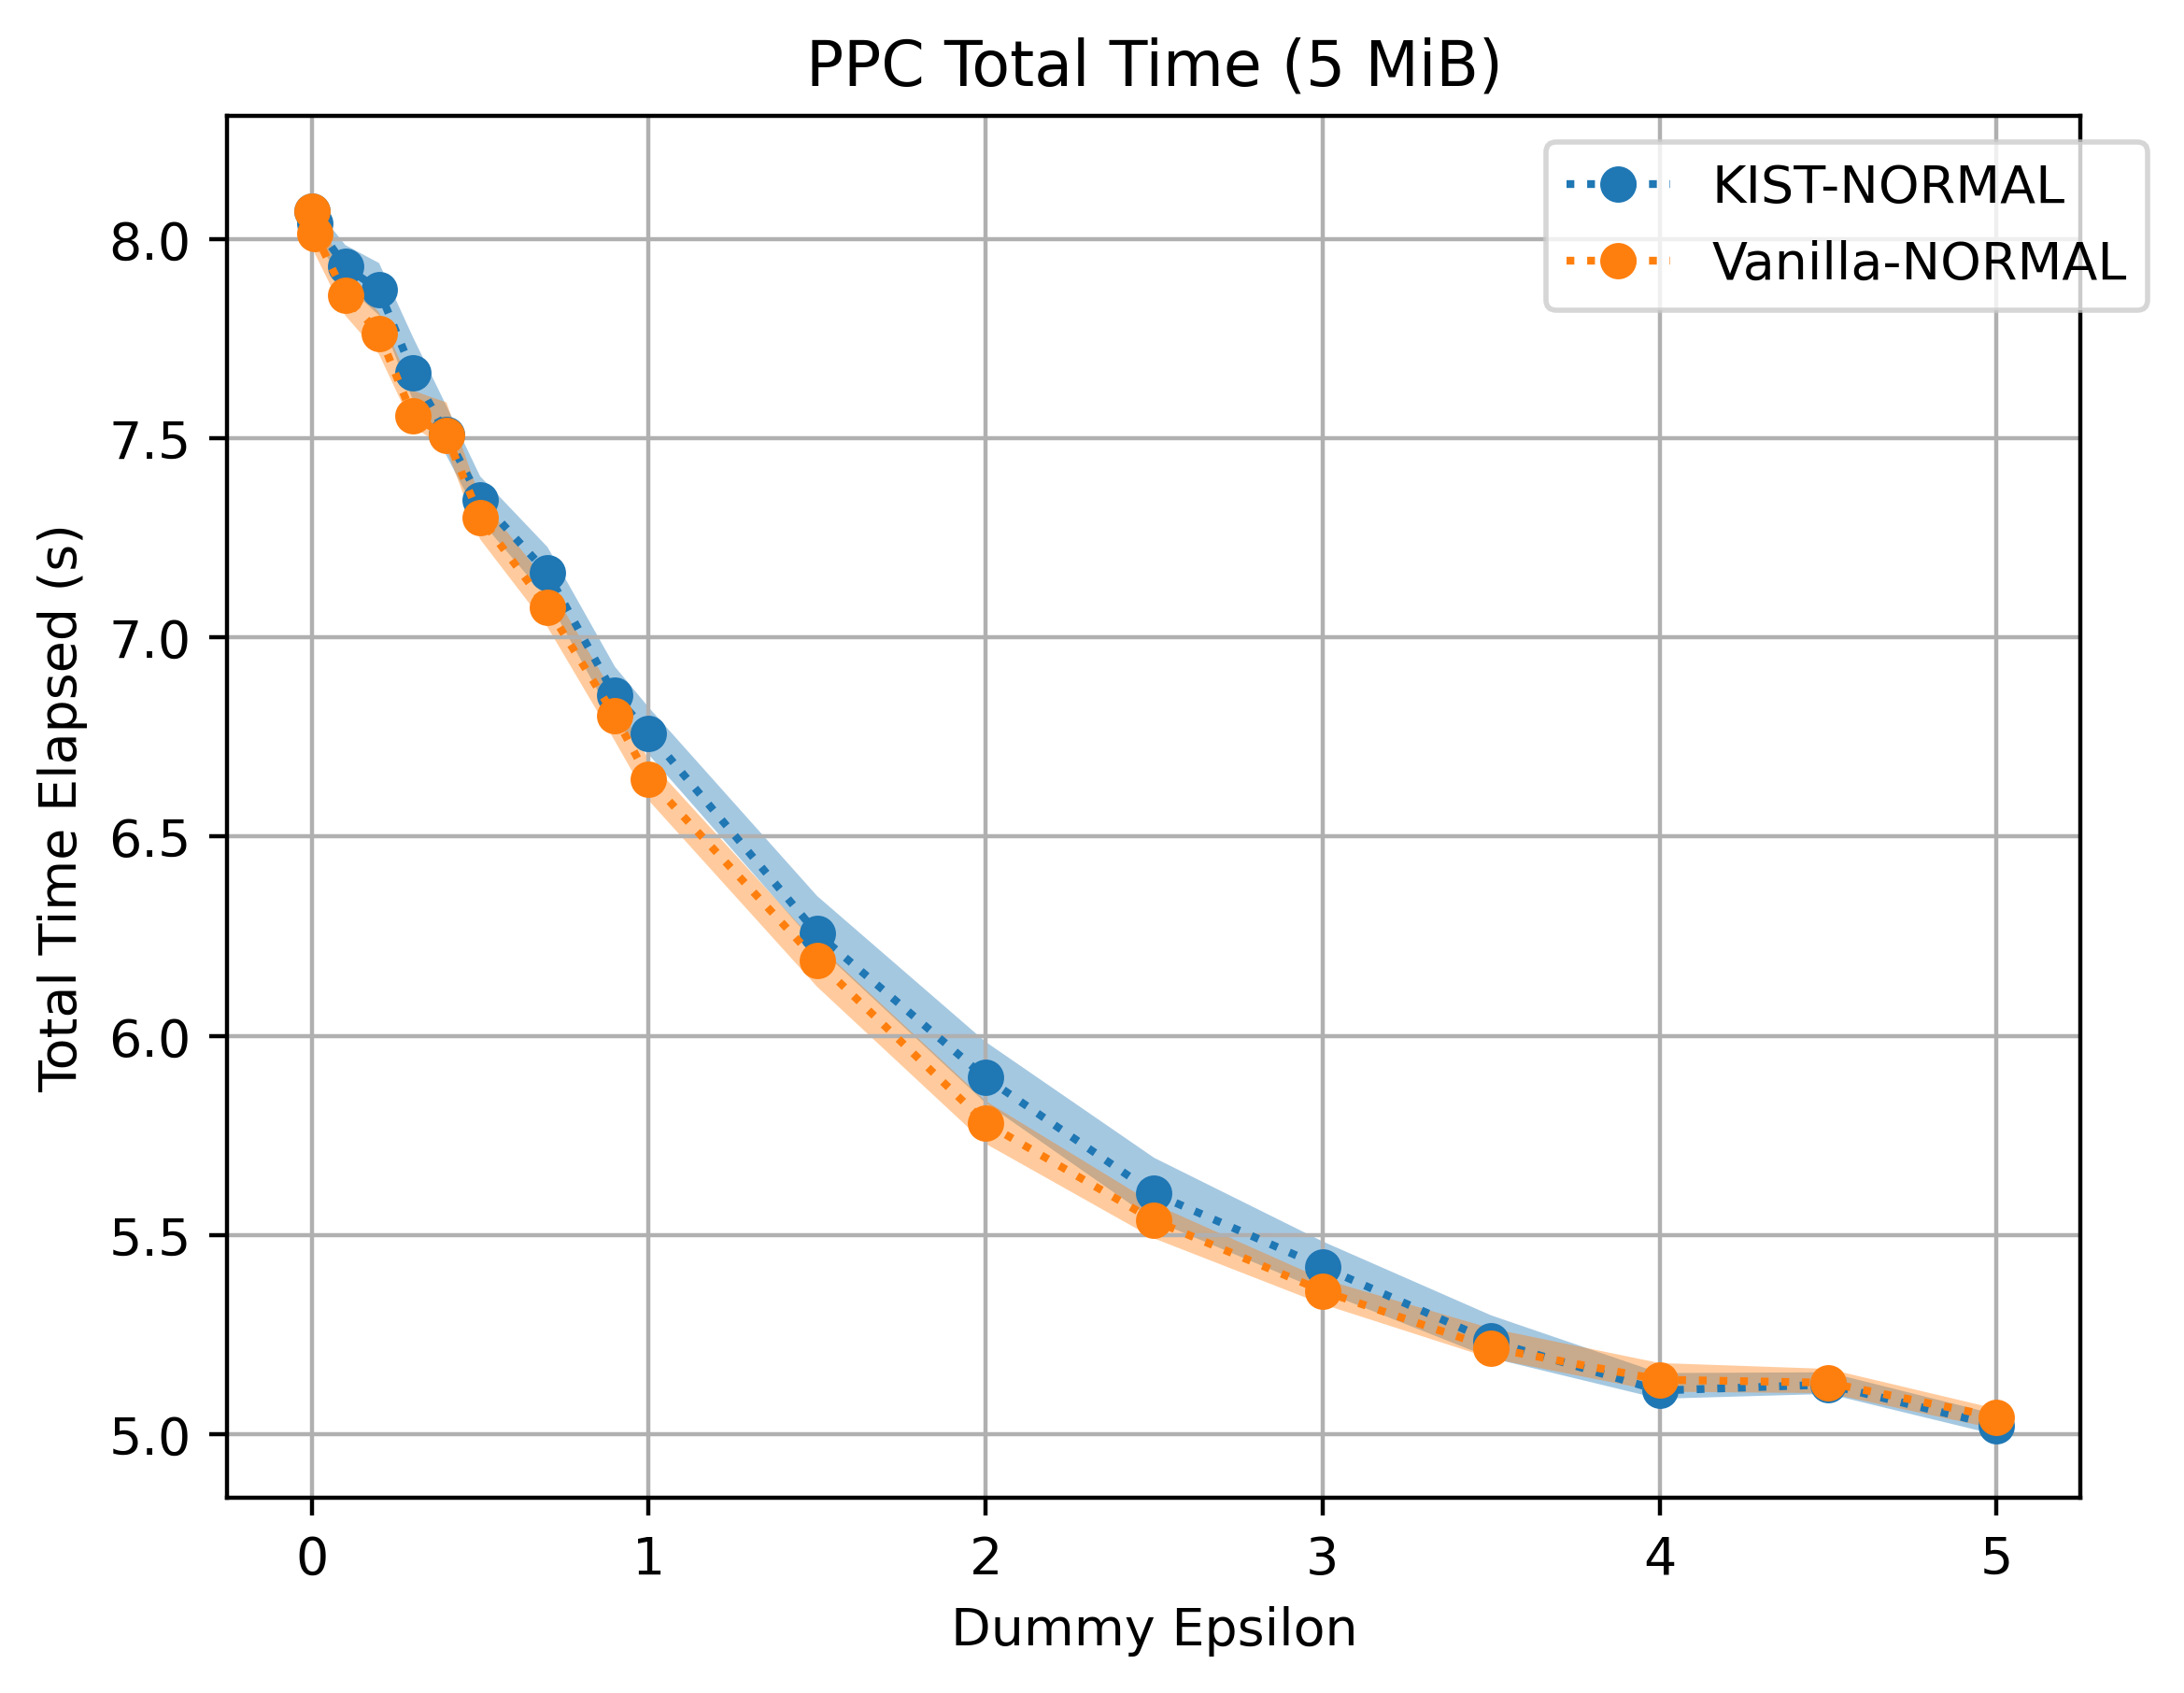
\includegraphics[width=\linewidth]{Chapters/Figures/Plots/local_total_time_50_PPC_5mib.png}}
    \end{subcaptionbox}
    \hfill
    \begin{subcaptionbox}{Only Jitter Injection Schedulers Feature\label{fig:local_jitter_total_time}}[0.45\textwidth]
        {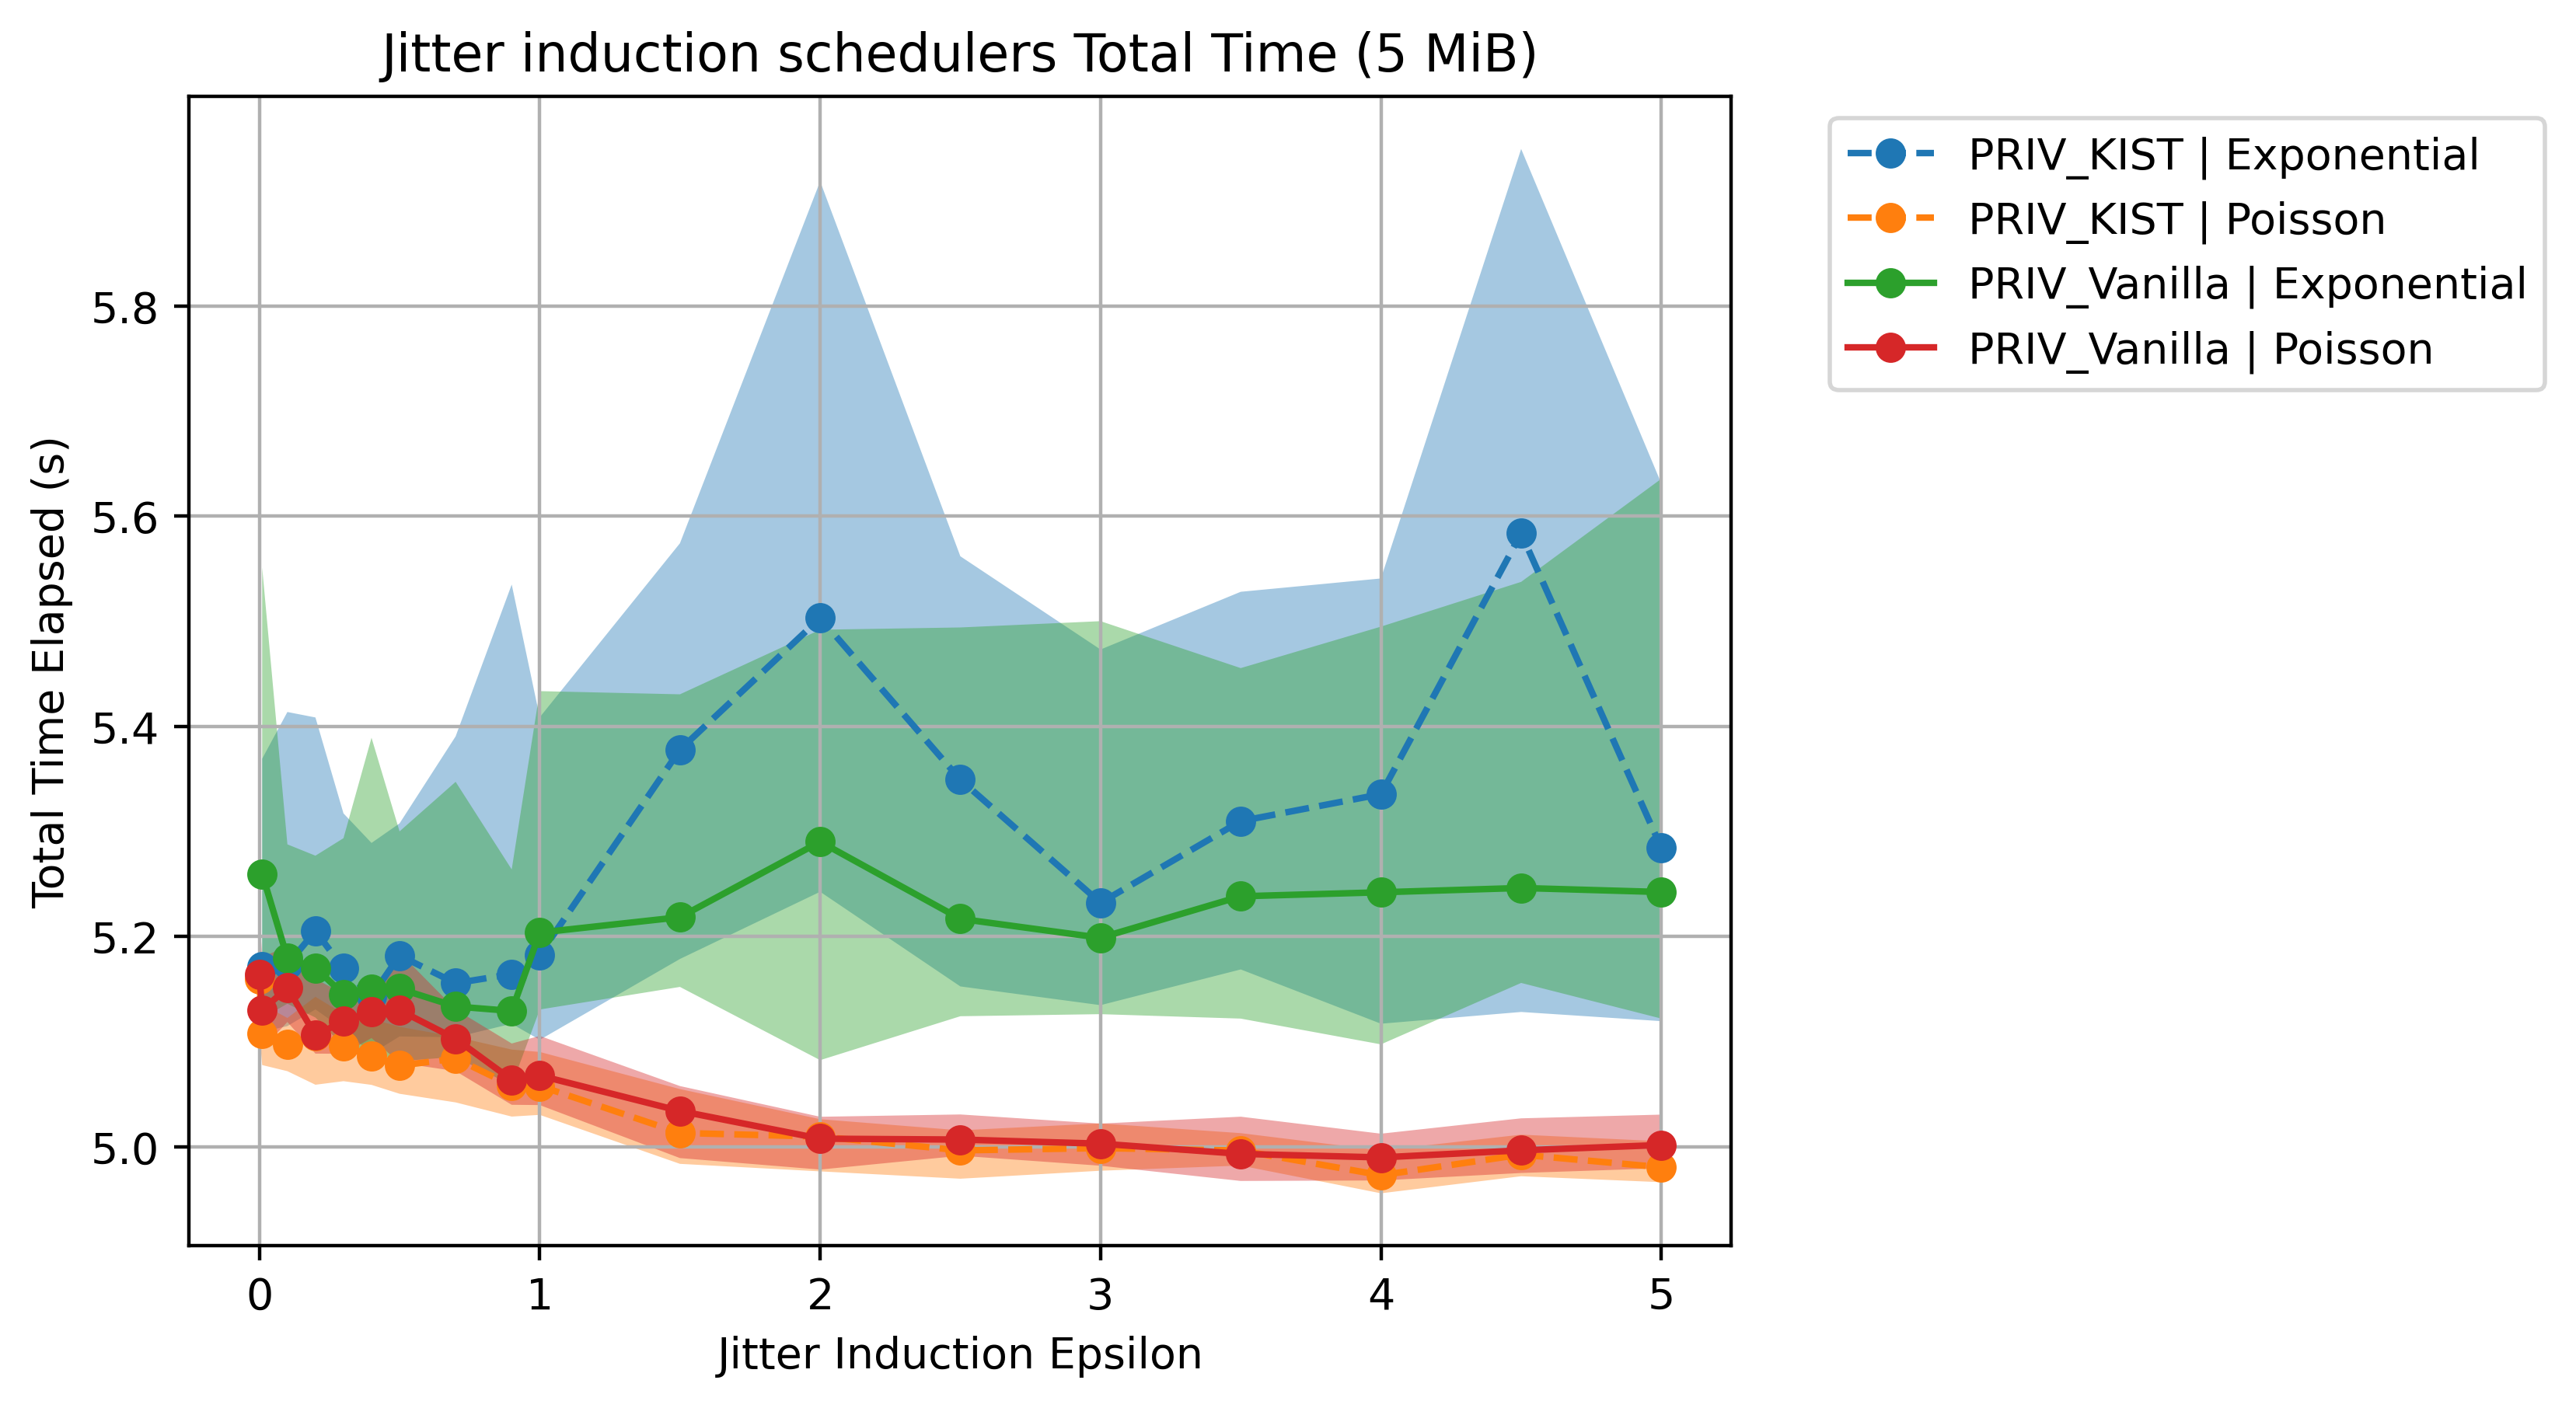
\includegraphics[width=\linewidth]{Chapters/Figures/Plots/local_total_time_50_jitter_5mib.png}}
    \end{subcaptionbox}
    \vfill
    \begin{subcaptionbox}{Both Features\label{fig:local_both_total_time}}[0.70\textwidth]
        {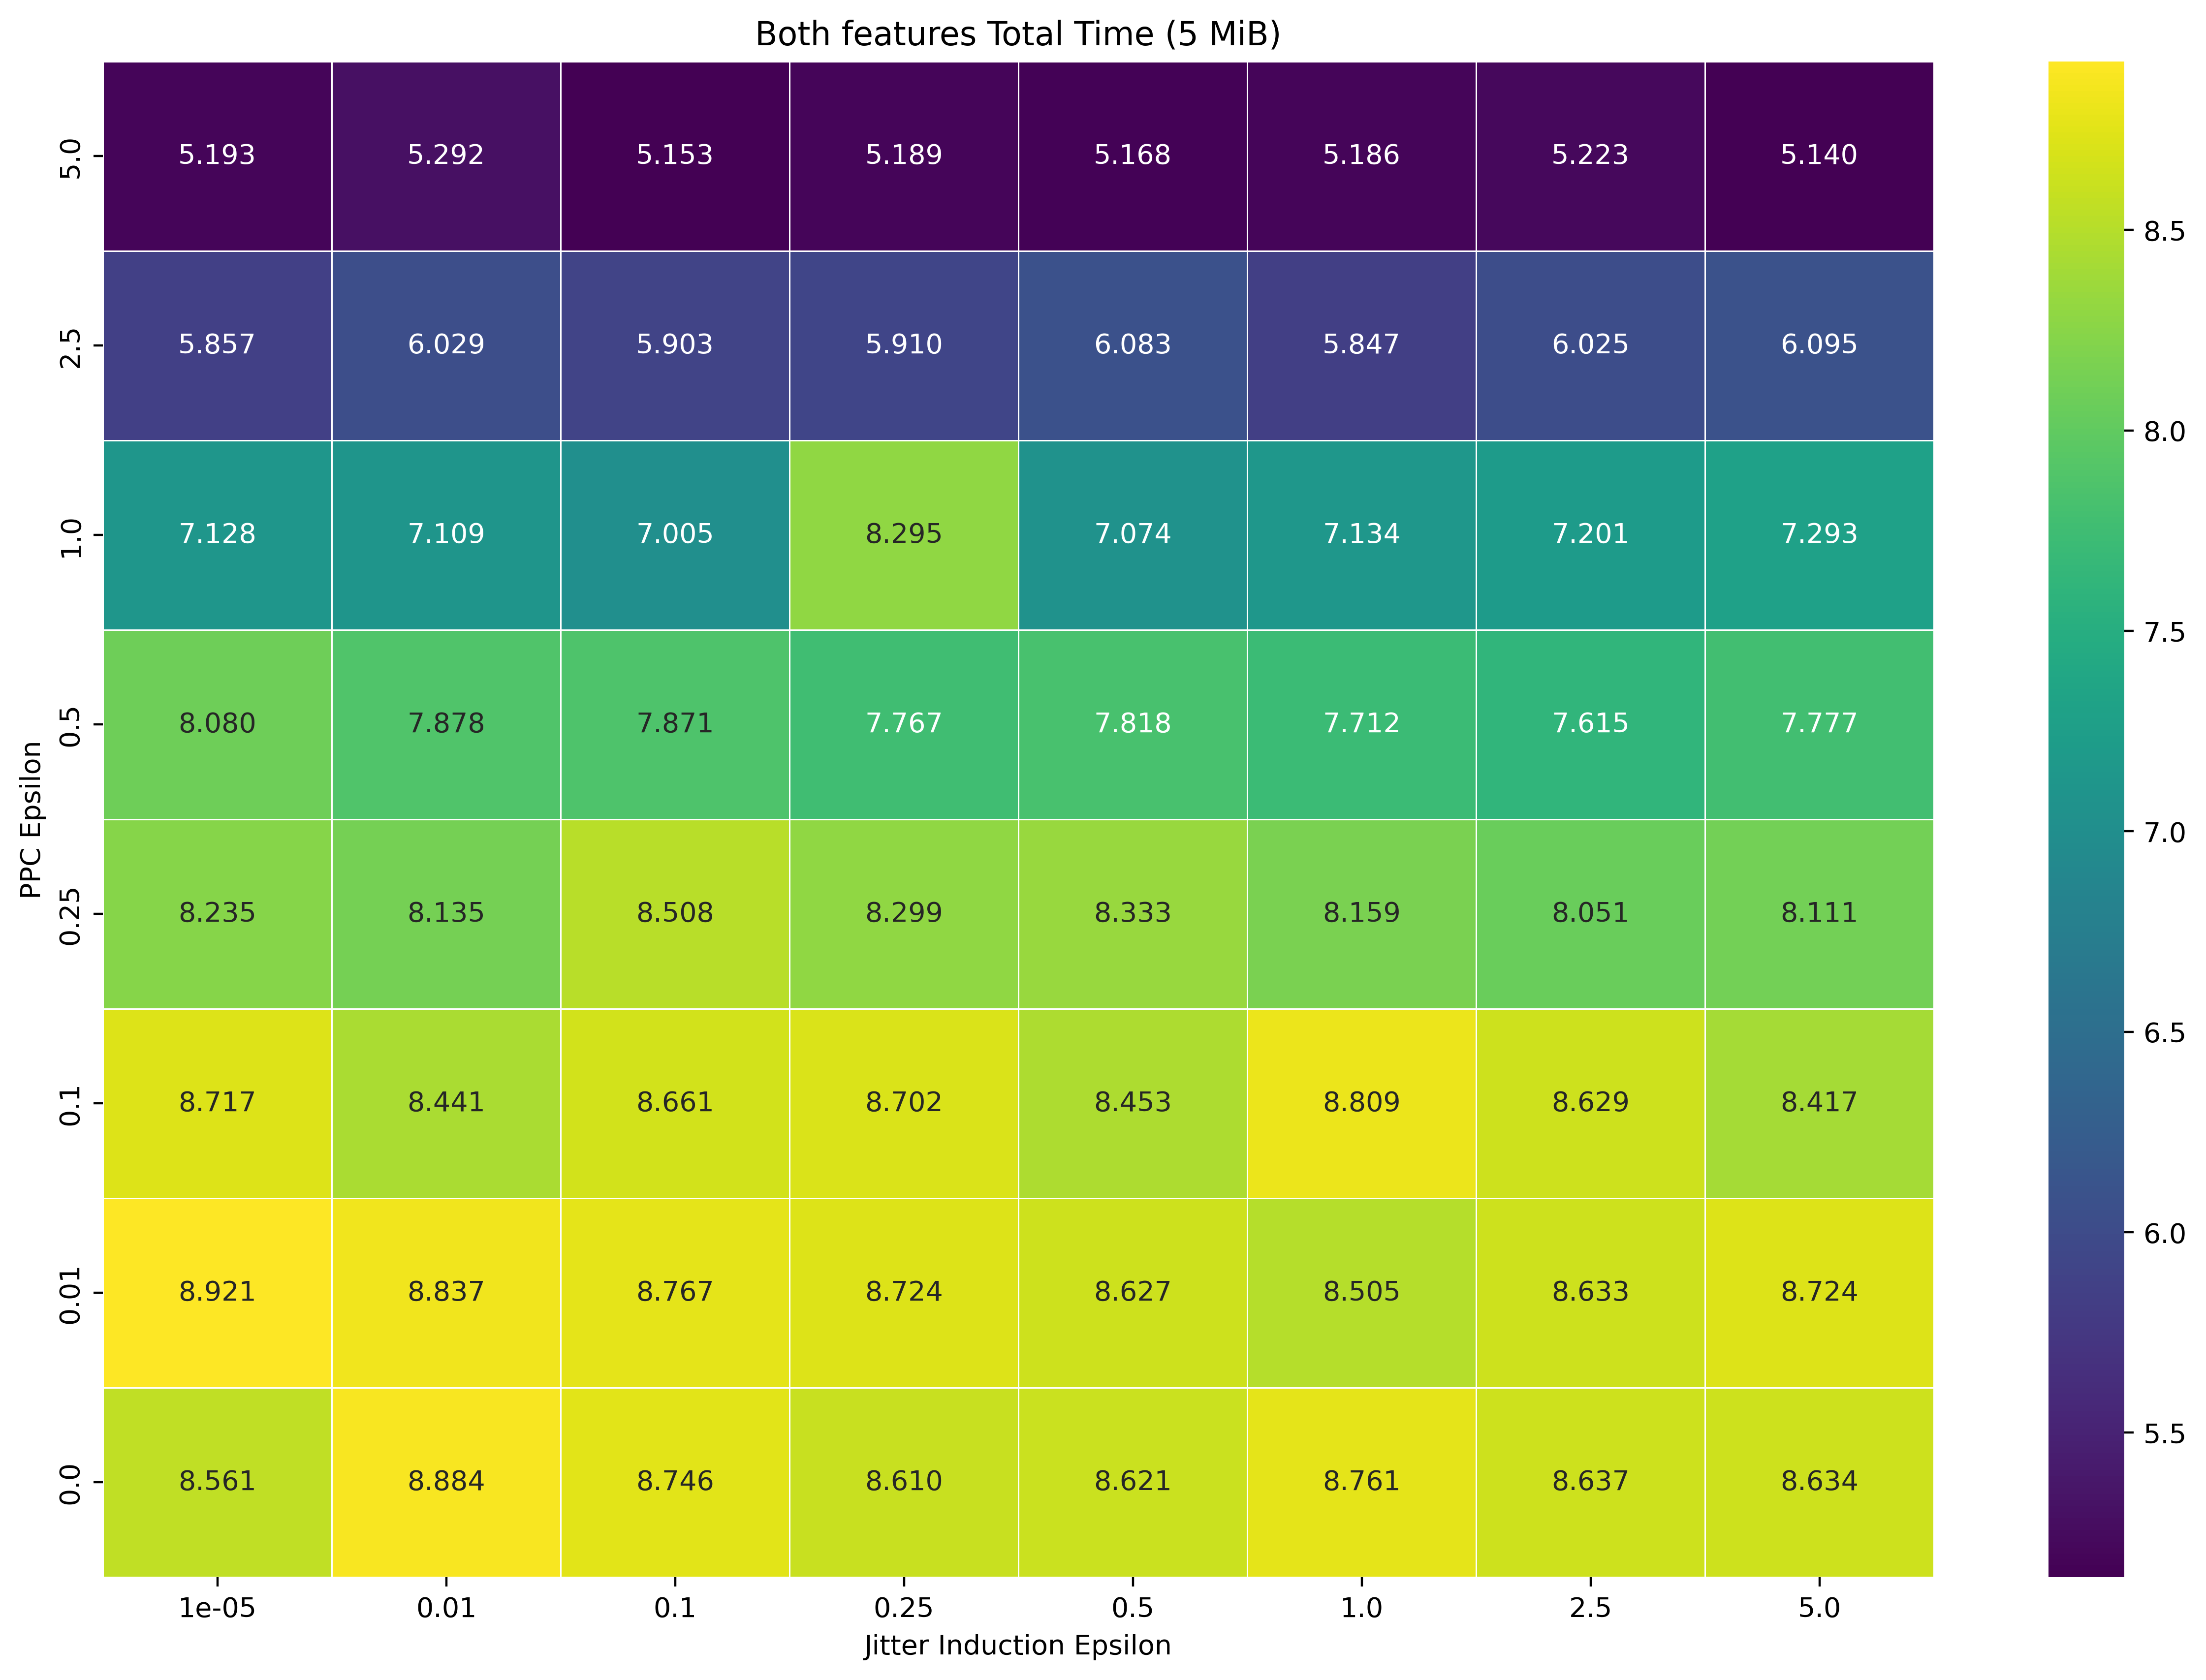
\includegraphics[width=\linewidth]{Chapters/Figures/Plots/local_total_time_50_heatmap_5mib.png}}
    \end{subcaptionbox}
    \caption{Total Time Results on Local Simulated Environment}\label{fig:local_total_time}
\end{figure}

\begin{figure}[htbp]
    \centering
    \begin{subcaptionbox}{Only Packet Padding Cells Feature\label{fig:dist_ppc_total_time}}[0.45\textwidth]
        {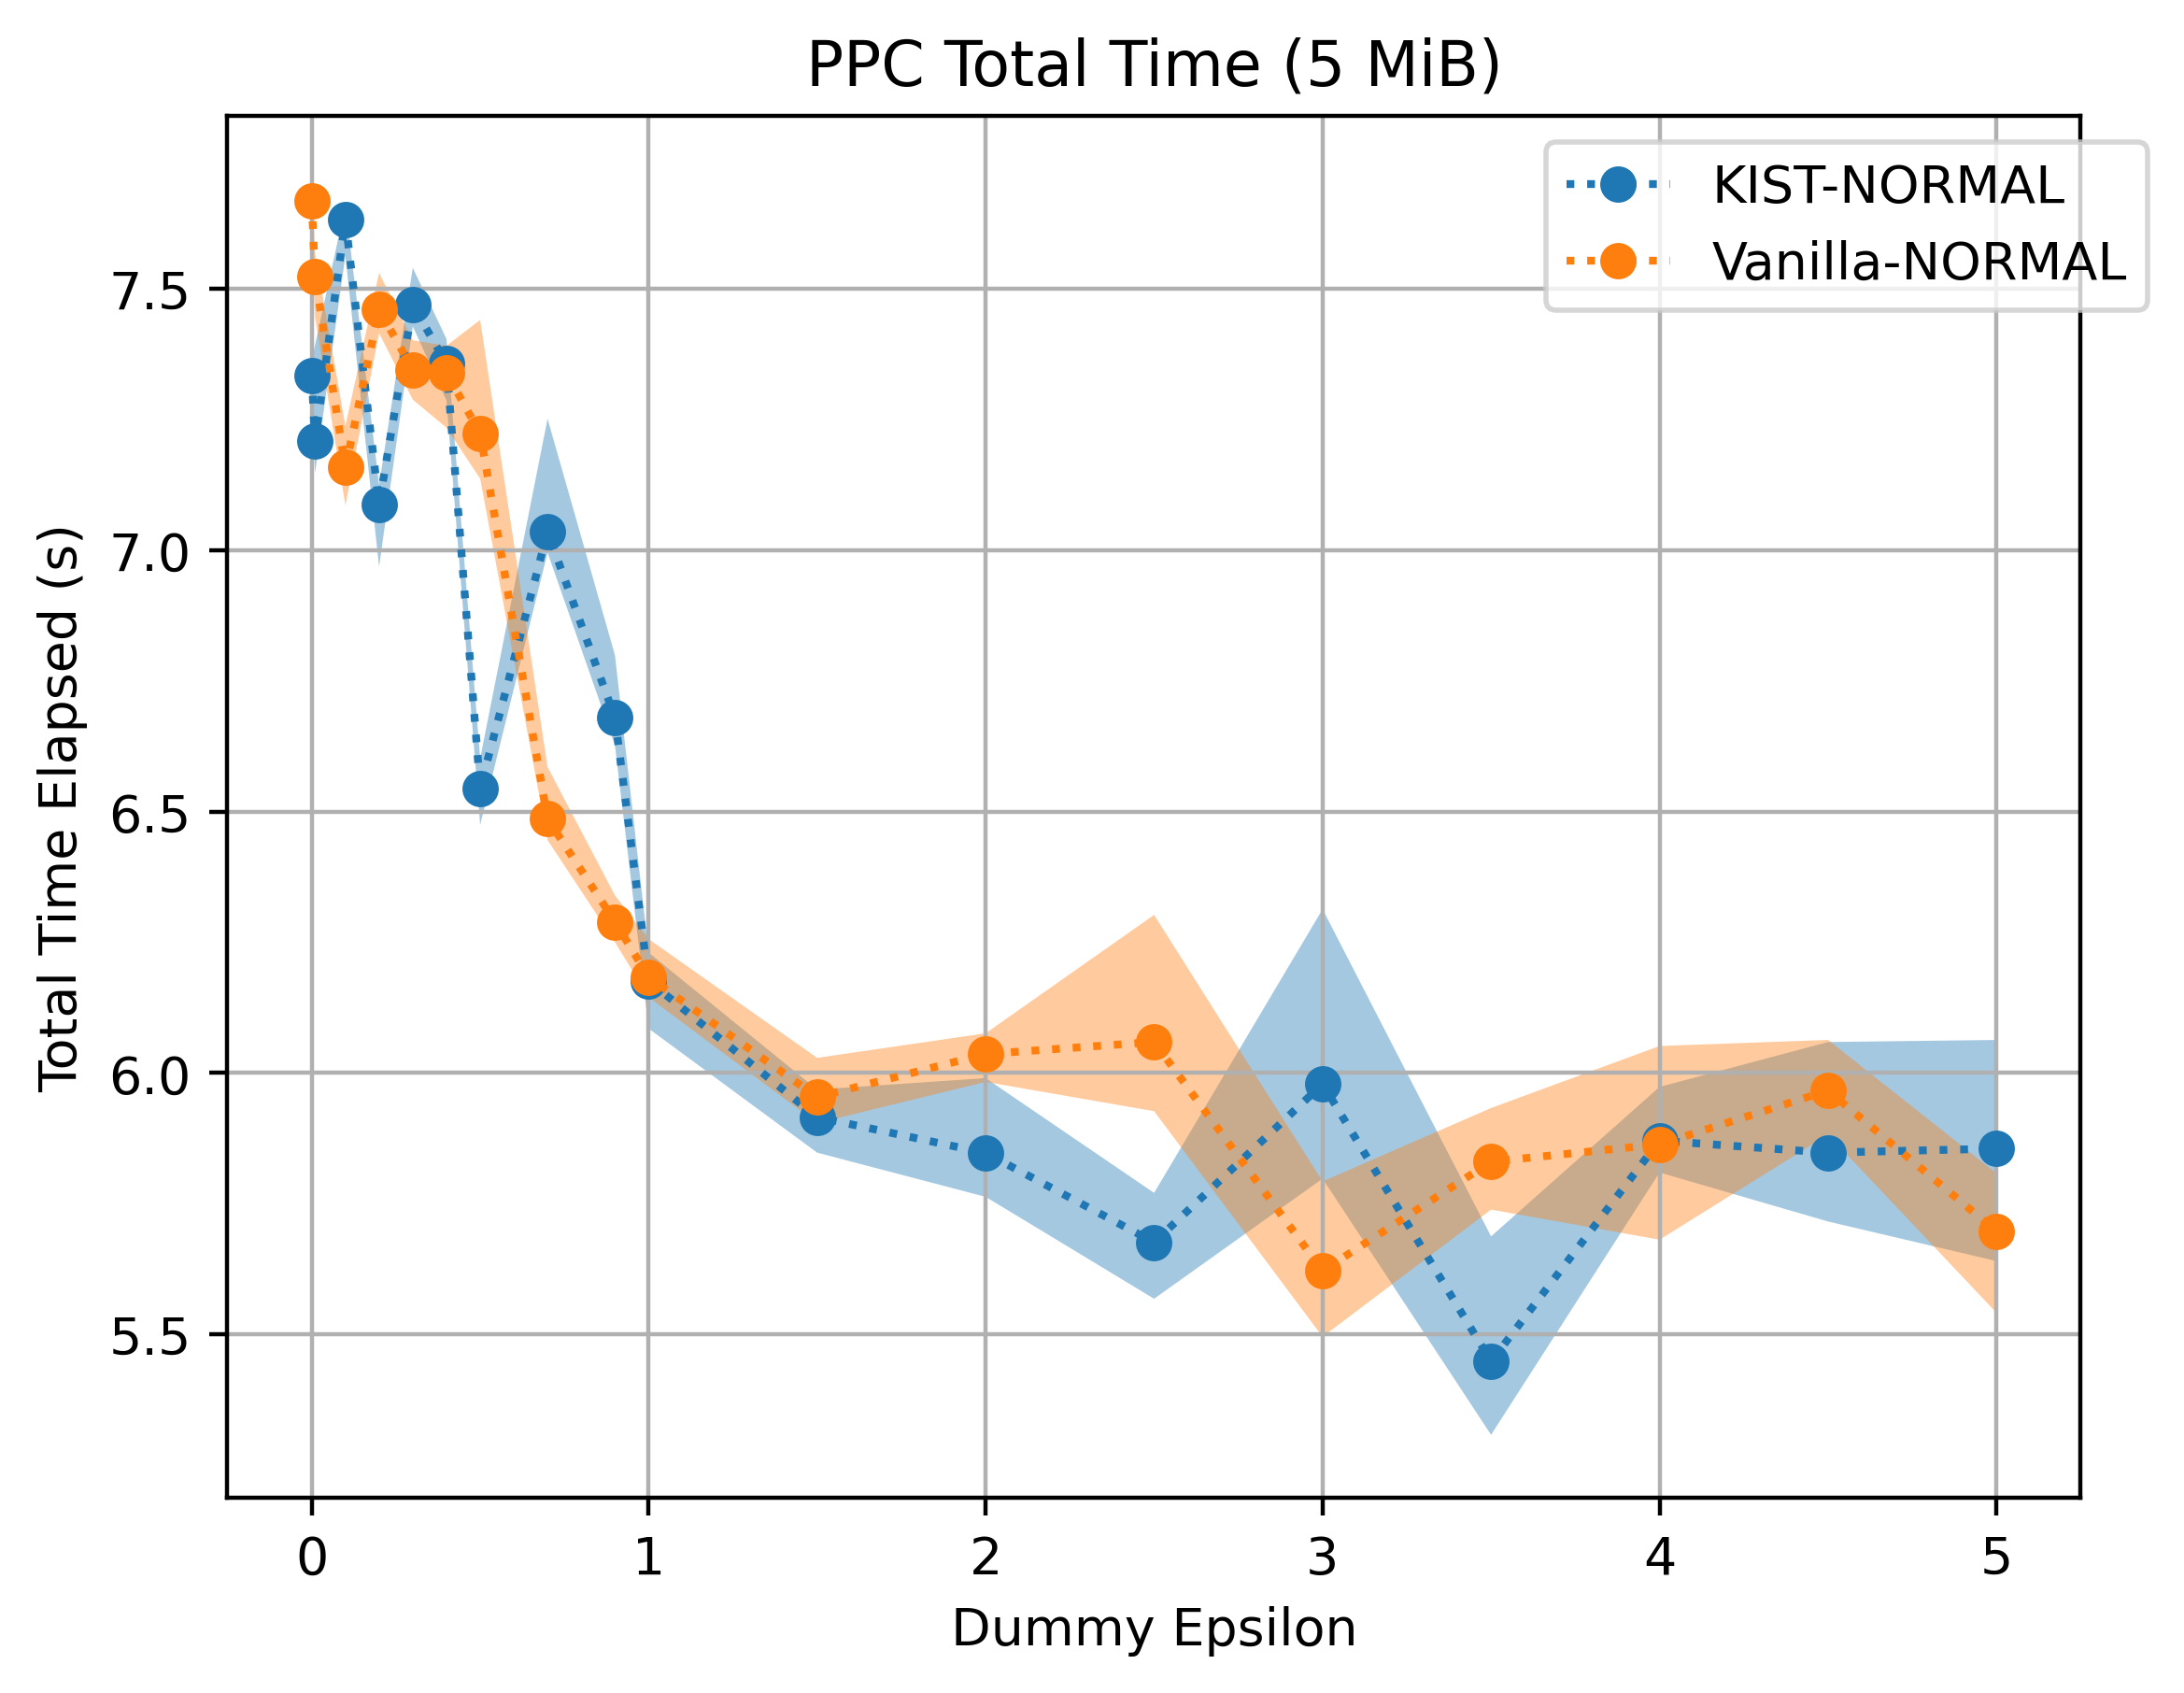
\includegraphics[width=\linewidth]{Chapters/Figures/Plots/dist_total_time_50_PPC_5mib.png}}
    \end{subcaptionbox}
    \hfill
    \begin{subcaptionbox}{Only Jitter Injection Schedulers Feature\label{fig:dist_jitter_total_time}}[0.45\textwidth]
        {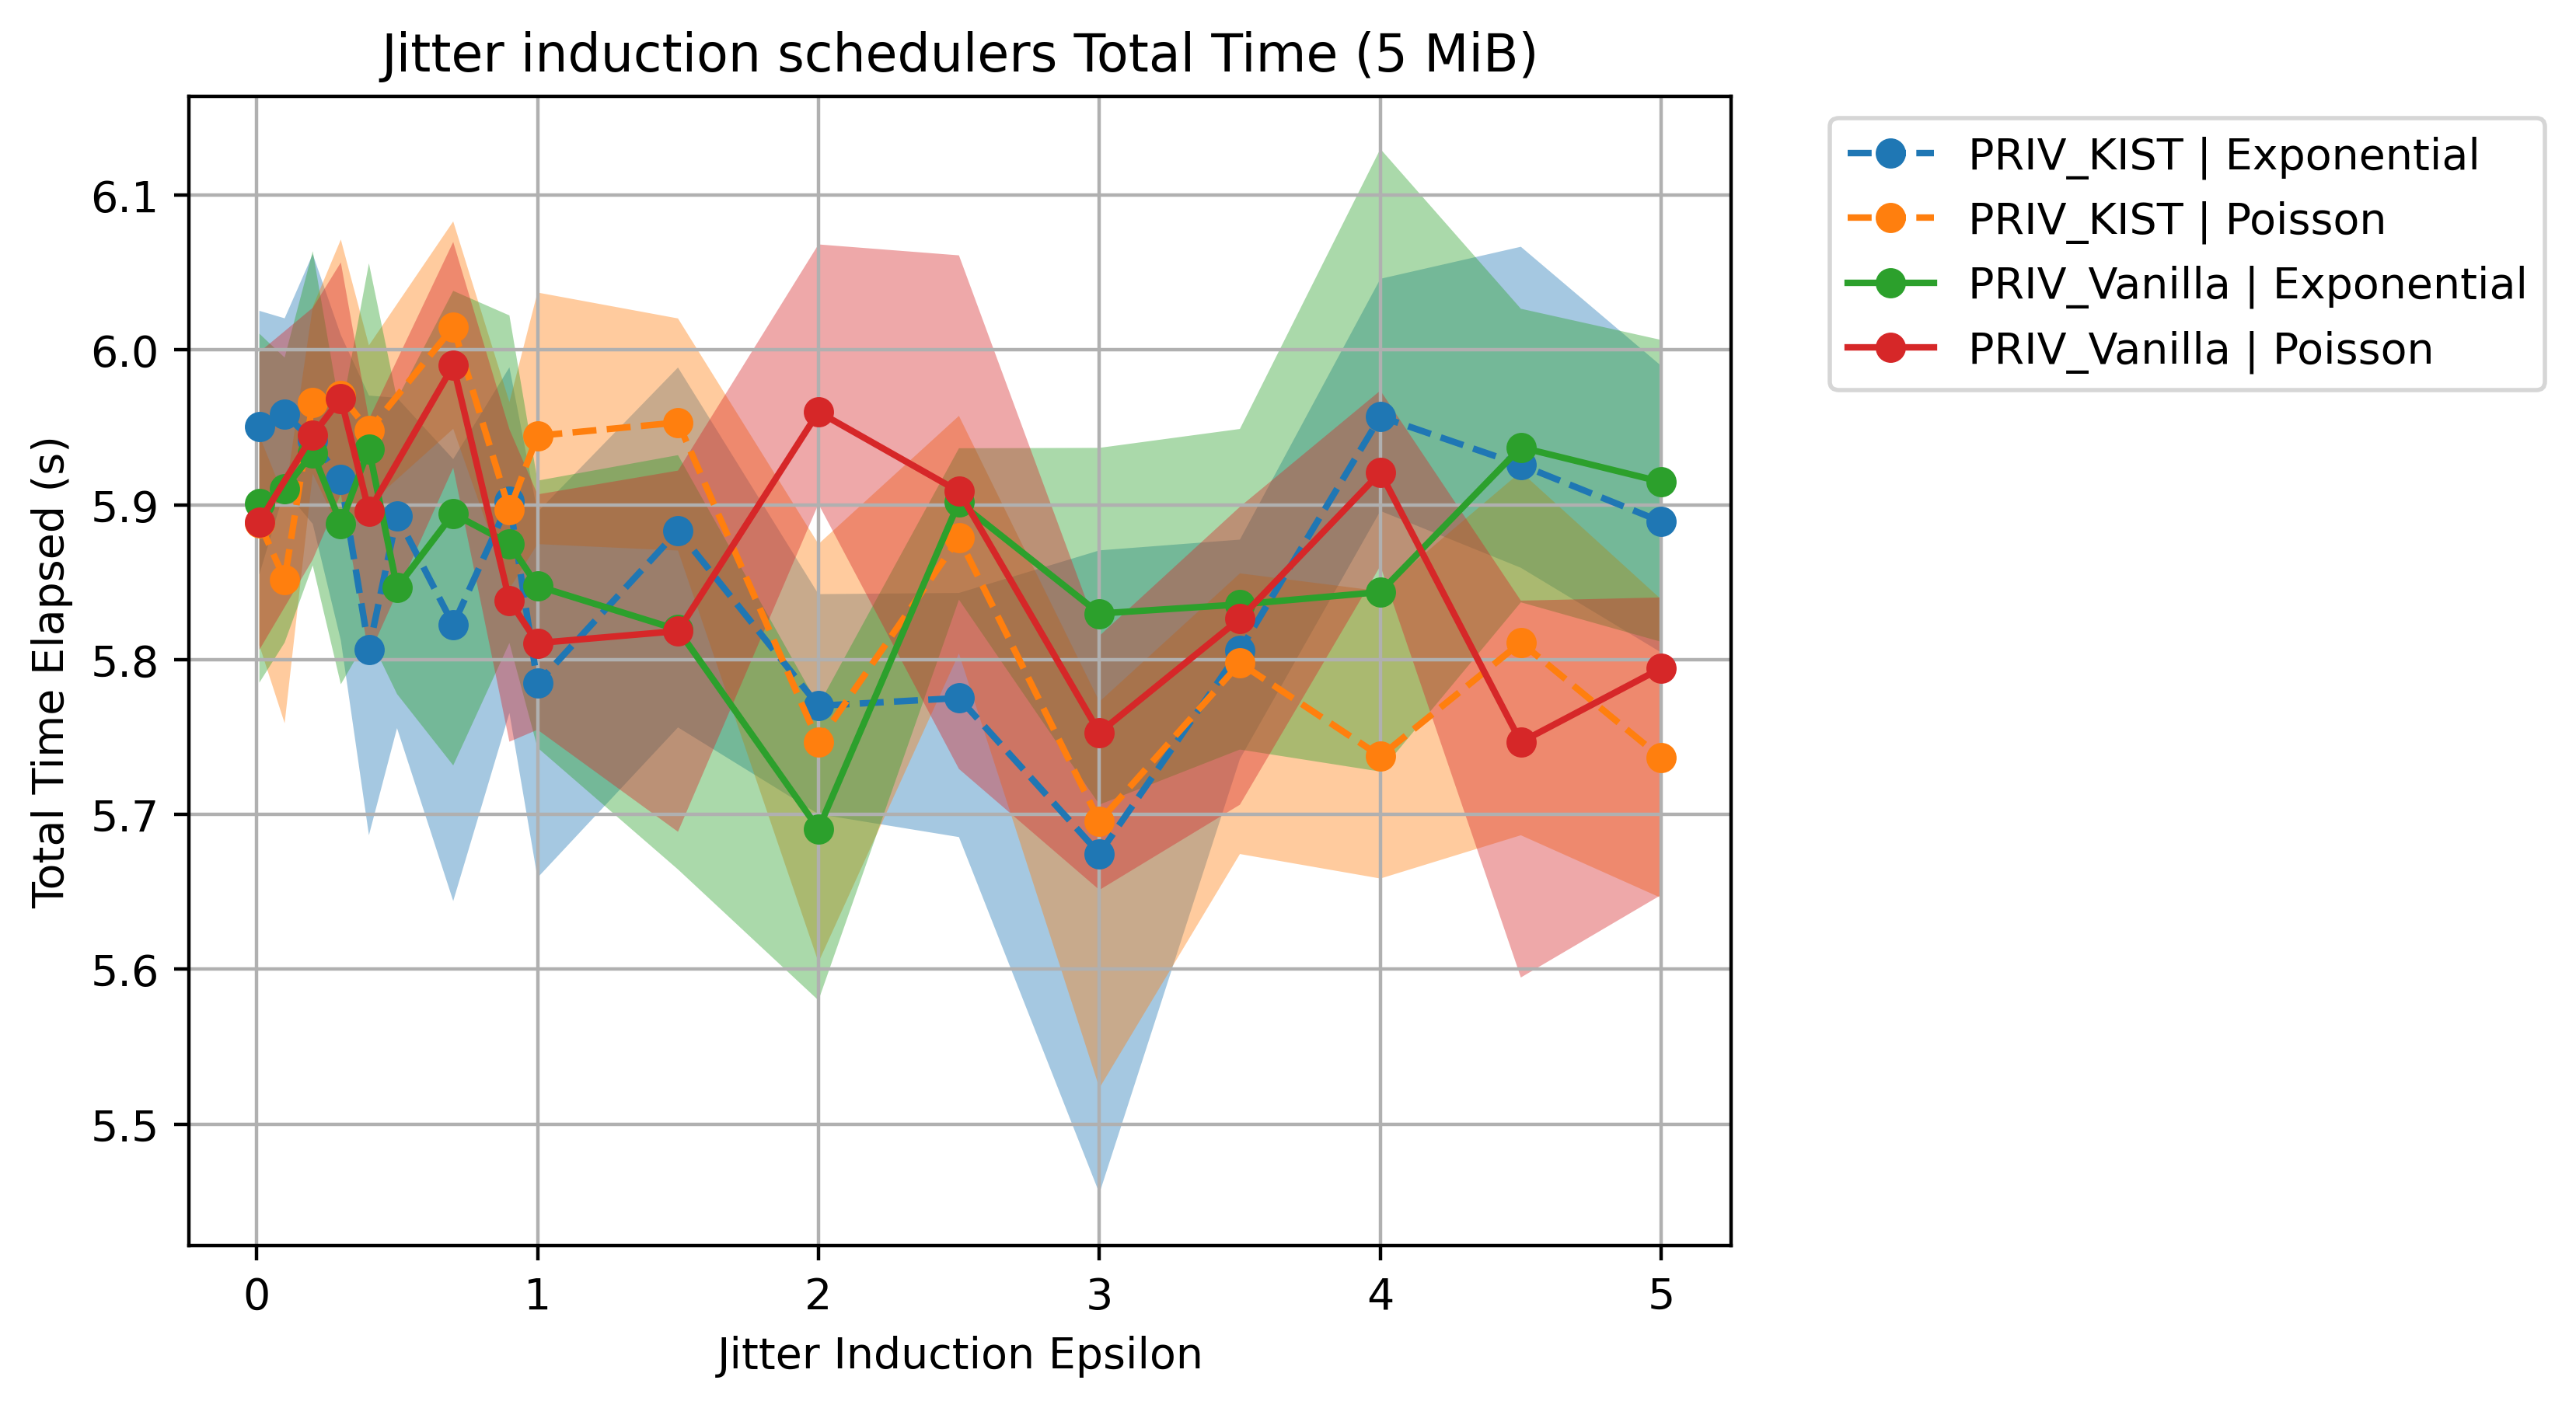
\includegraphics[width=\linewidth]{Chapters/Figures/Plots/dist_total_time_50_jitter_5mib.png}}
    \end{subcaptionbox}
    \vfill
    \begin{subcaptionbox}{Both Features\label{fig:dist_both_total_time}}[0.70\textwidth]
        {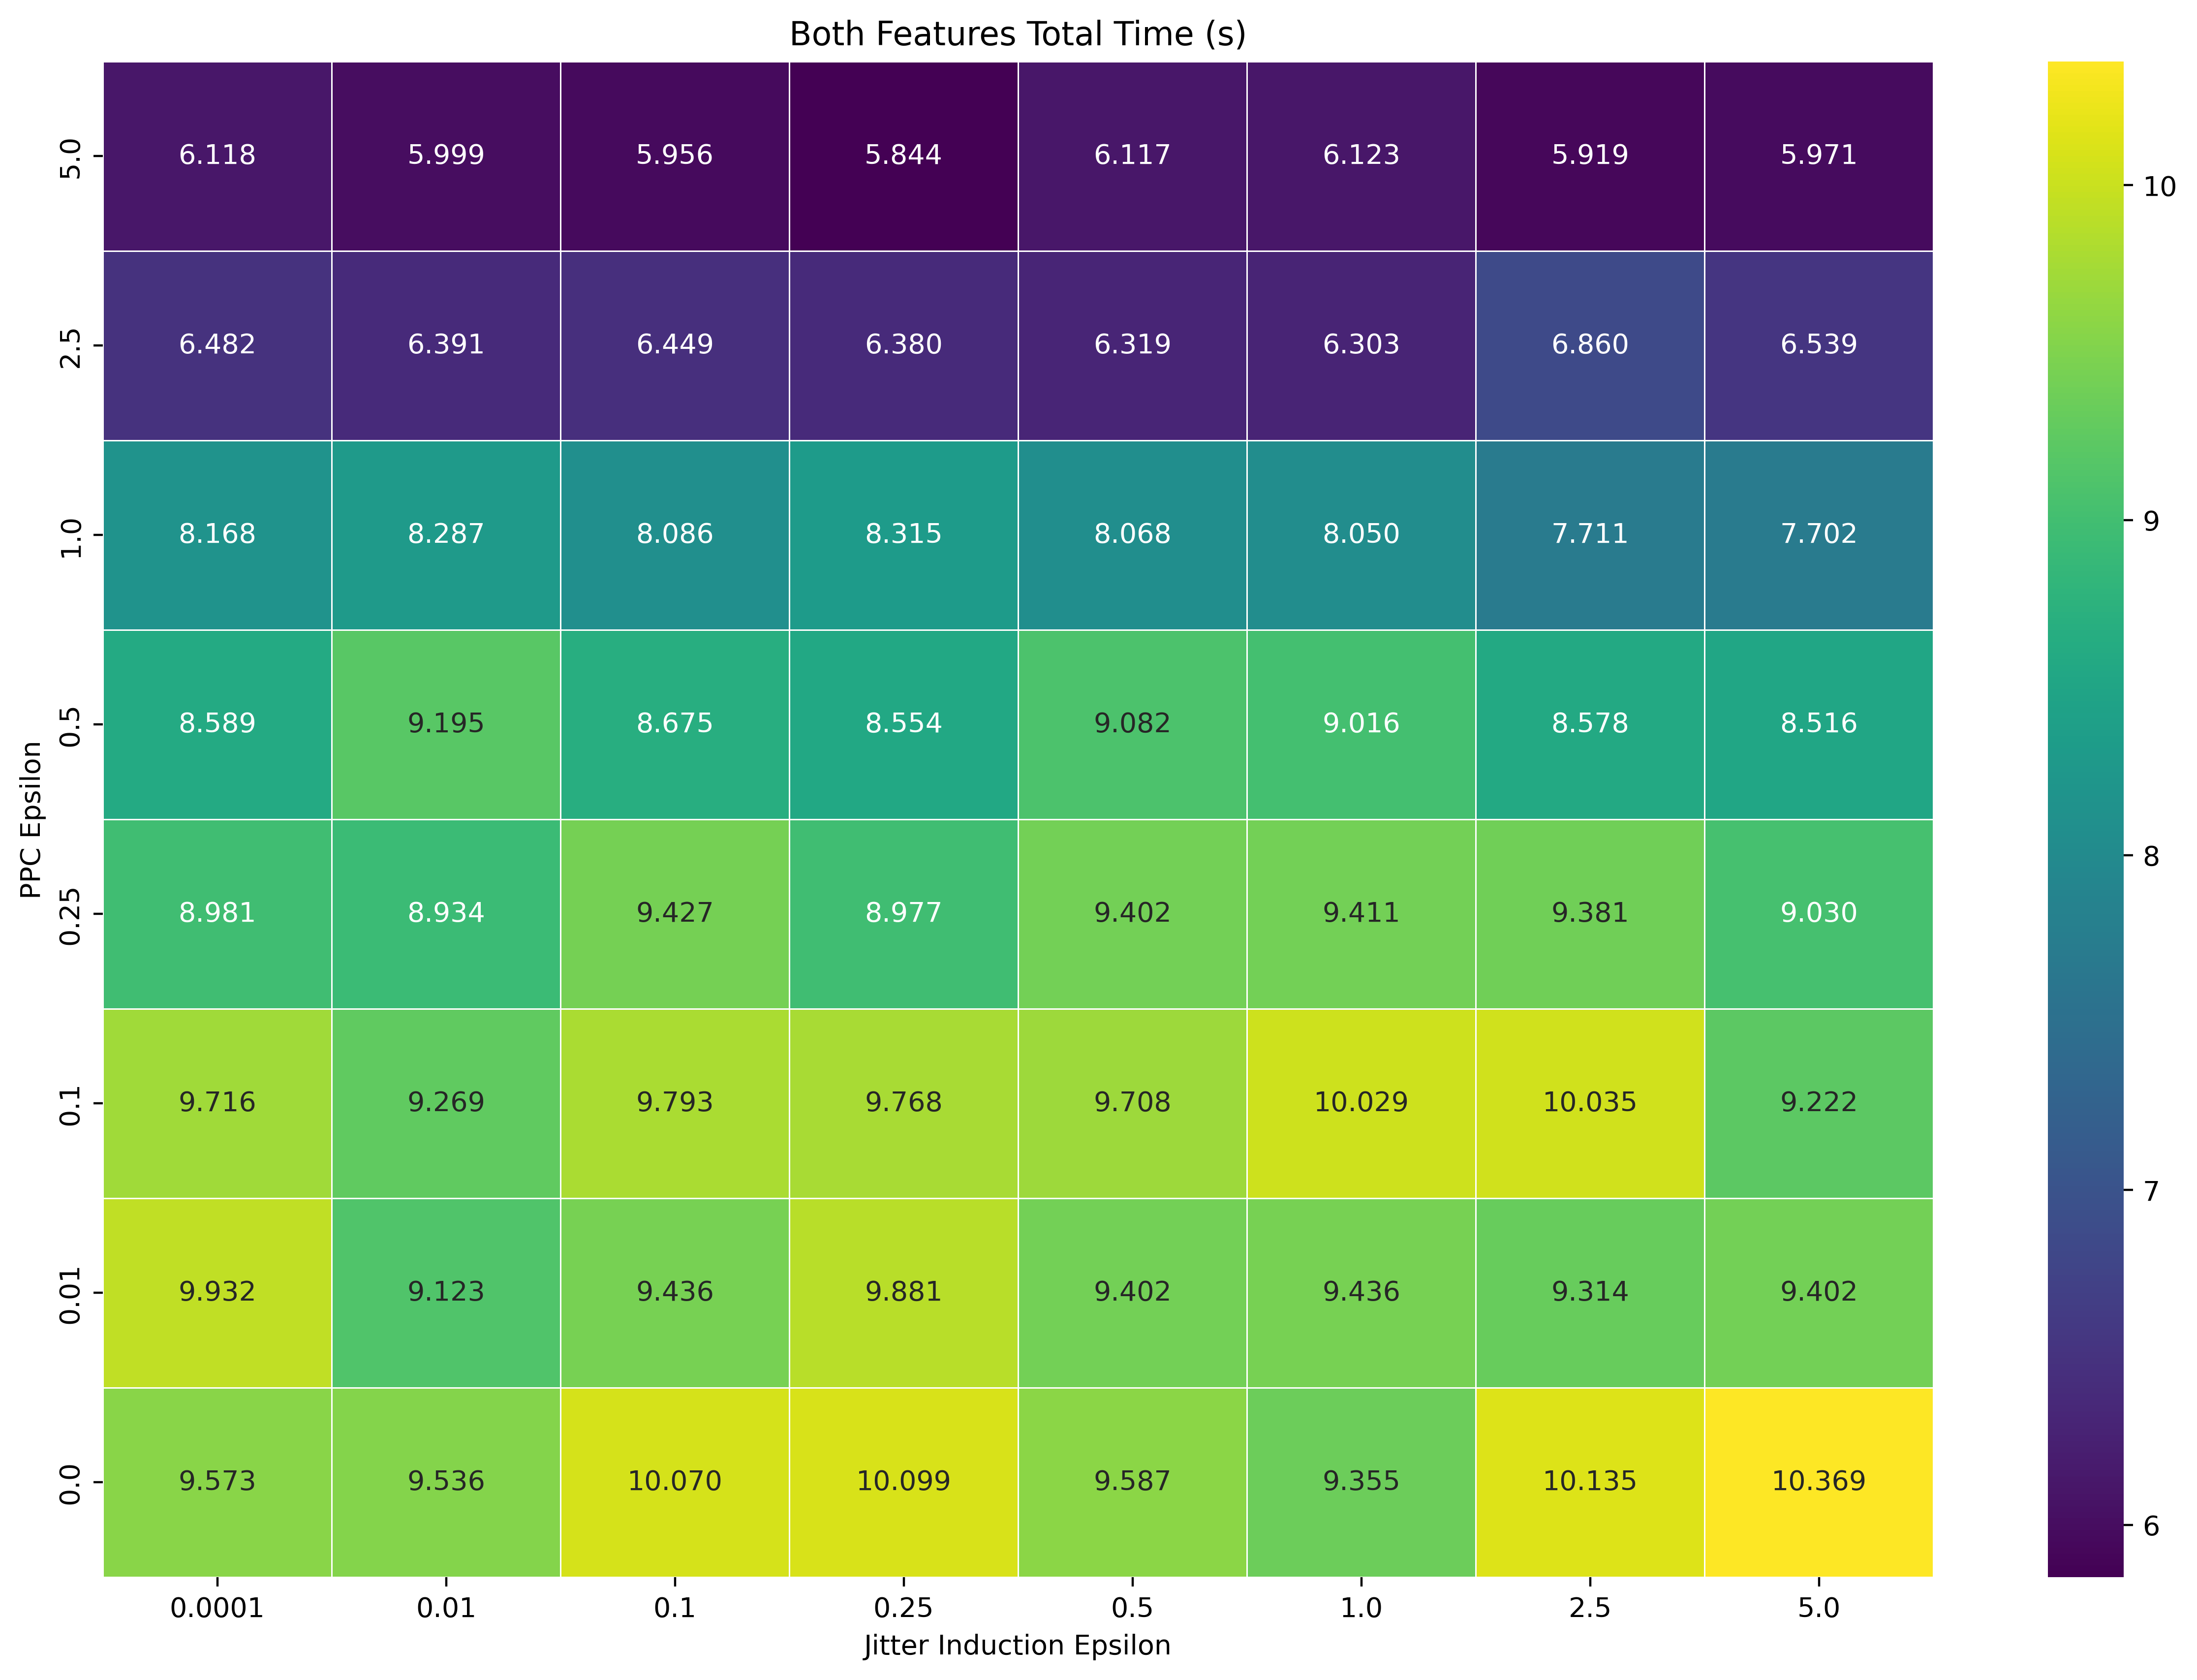
\includegraphics[width=\linewidth]{Chapters/Figures/Plots/dist_total_time_50_heatmap_5mib.png}}
    \end{subcaptionbox}
    \caption{Total Time Results on Distributed Environment}\label{fig:dist_total_time}
\end{figure}

As demonstrated in~\autoref{fig:local_total_time} and~\autoref{fig:dist_total_time}, the total time to download a file got results proportional to the throughput results, meaning that the PPC feature significantly influenced the total time to download. Regarding the Packet Padding Cells feature, the total time experienced is significantly lower as $\epsilon_{PPC}$ decreases. The same can be said about the Schedulers feature, although the impact is smaller. Additionally, the Exponential distribution showed a higher variance in the local test bench, and the median results unexpectably increased 0.1 seconds. This situation got normalized in the distributed test bench.   
Both schedulers behaved similarly in all experiments, thus we used the KIST variant and the Poisson distribution to test both features together. The results of the combined features also emphasized the greater impact of the PPC feature on the total time to download a file. Alike the throughput results, the total time heatmap proves that the schedulers feature has a negligible impact on the total time, when compared with the PPC.\@
%TODO: MUST TEST COMBINATIONS ON DISTRIBUTED TO GET BETTER ANALYSIS ON WORSE/BETTER TEST BENCH AND CONFIGURATION
\begin{table}[htbp]
    \centering
    \begin{tabular}{|c|c|c|}
    \hline
    \textbf{Configuration} & \textbf{Local} & \textbf{Distributed} \\
    \hline
    Tor Metrics &  \multicolumn{2}{c|}{4.825} \\ 
    \hline
    \multirow{2}{*}{Control} & 5.09 & 5.95\\ 
    & 5.09 & 5.75\\
    \hline
    Only PPC & 5.02 – 8.07 & 5.45 – 7.67\\
    \hline
    Only Jitter & 5.58 – 4.97 & 5.67 – 6.01\\
    \hline
    PPC \& Jitter & 5.13 – 8.88 & 5.87 – 6.32\\
    \hline
    \end{tabular}
    \caption{Total Time Results Summary (s)}\label{tab:total_time_summary}
\end{table}

\FloatBarrier
\subsection{Latency}

Tor Metrics defines their circuit round-trip latencies as the time between the HTTP request and the first byte of the HTTP response's header. This way, we obtained the latency results based on the time to the first byte of the HTTP response's header. This metric also represents a key aspect of a communication system such as Tor because it allows to understand the maximum rate information may be transmitted. 

Similarly to the previous metrics, we present the latency results obtained from our experiments in~\autoref{fig:local_latency} for the local simulated environment and~\autoref{fig:dist_latency} for the distributed environment. We followed the Tor Metrics directives and also present the results as a thick line which represents the median value, together with a shaded area representing the first and third quartiles.

\begin{figure}[htbp]
    \centering
    \begin{subcaptionbox}{Only Packet Padding Cells Feature\label{fig:local_ppc_latency}}[0.45\textwidth]
        {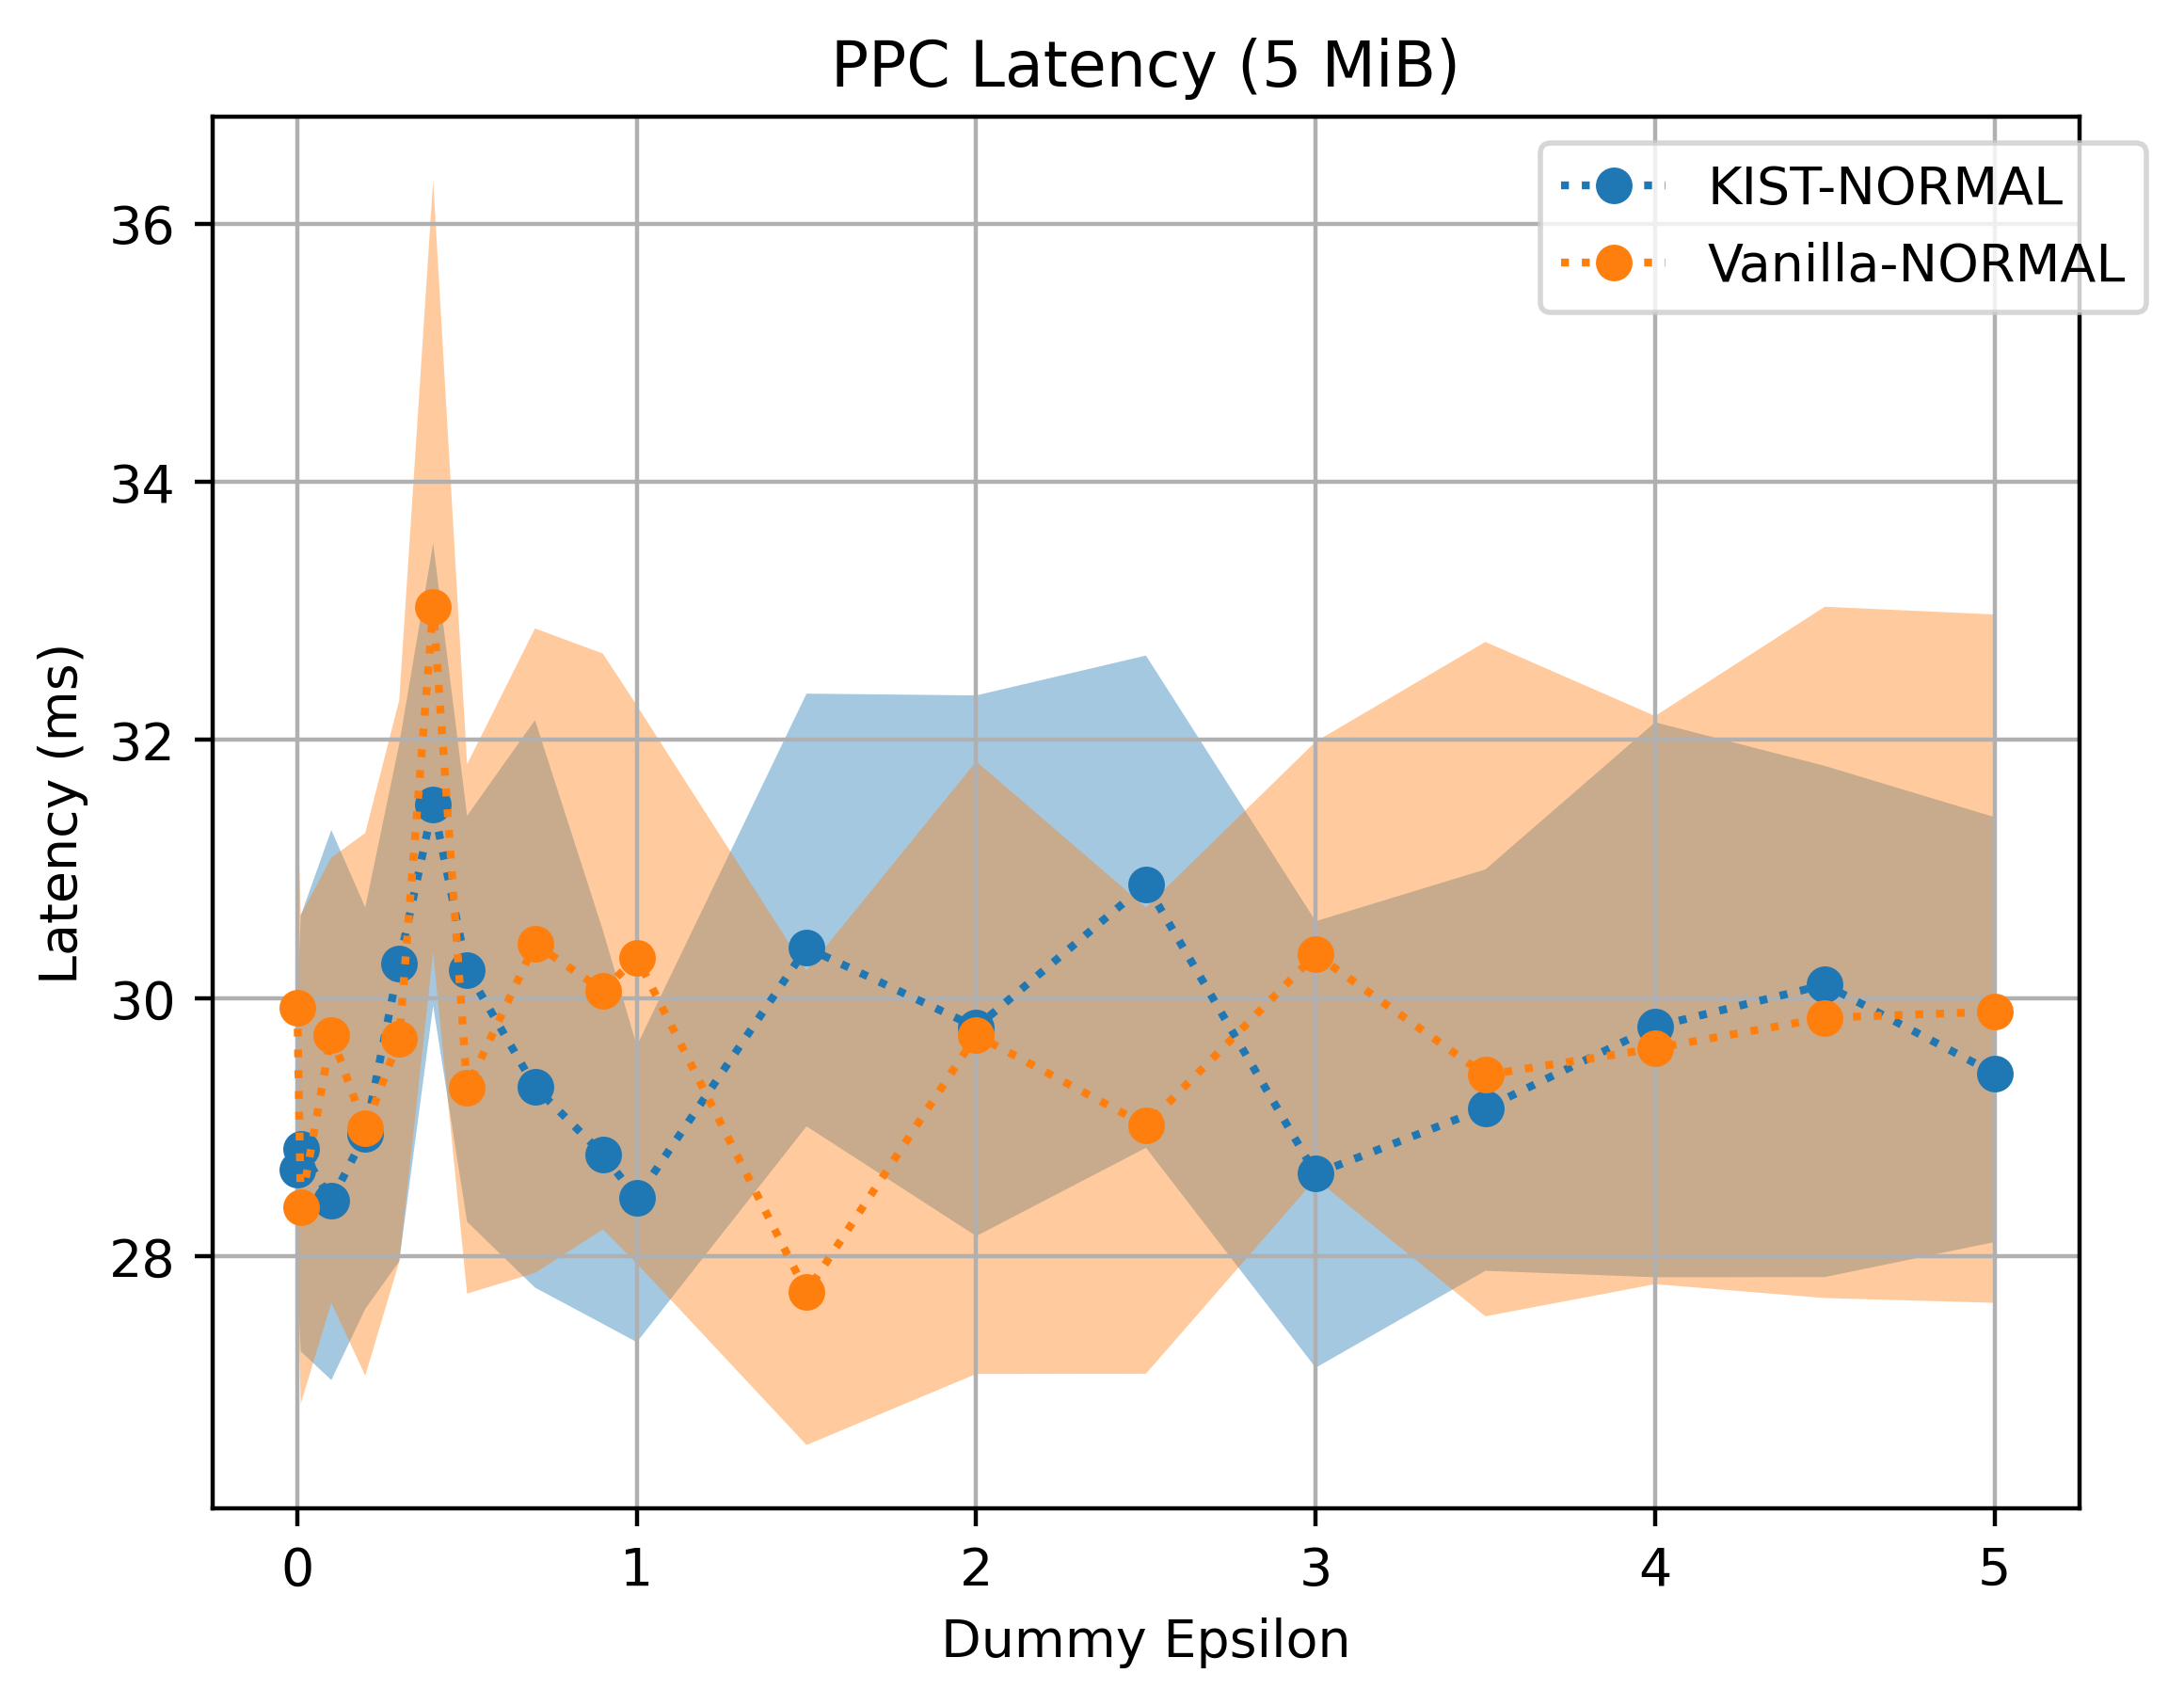
\includegraphics[width=\linewidth]{Chapters/Figures/Plots/local_latency_50_PPC_5mib.png}}
    \end{subcaptionbox}
    \hfill
    \begin{subcaptionbox}{Only Jitter Injection Schedulers Feature\label{fig:local_jitter_latency}}[0.45\textwidth]
        {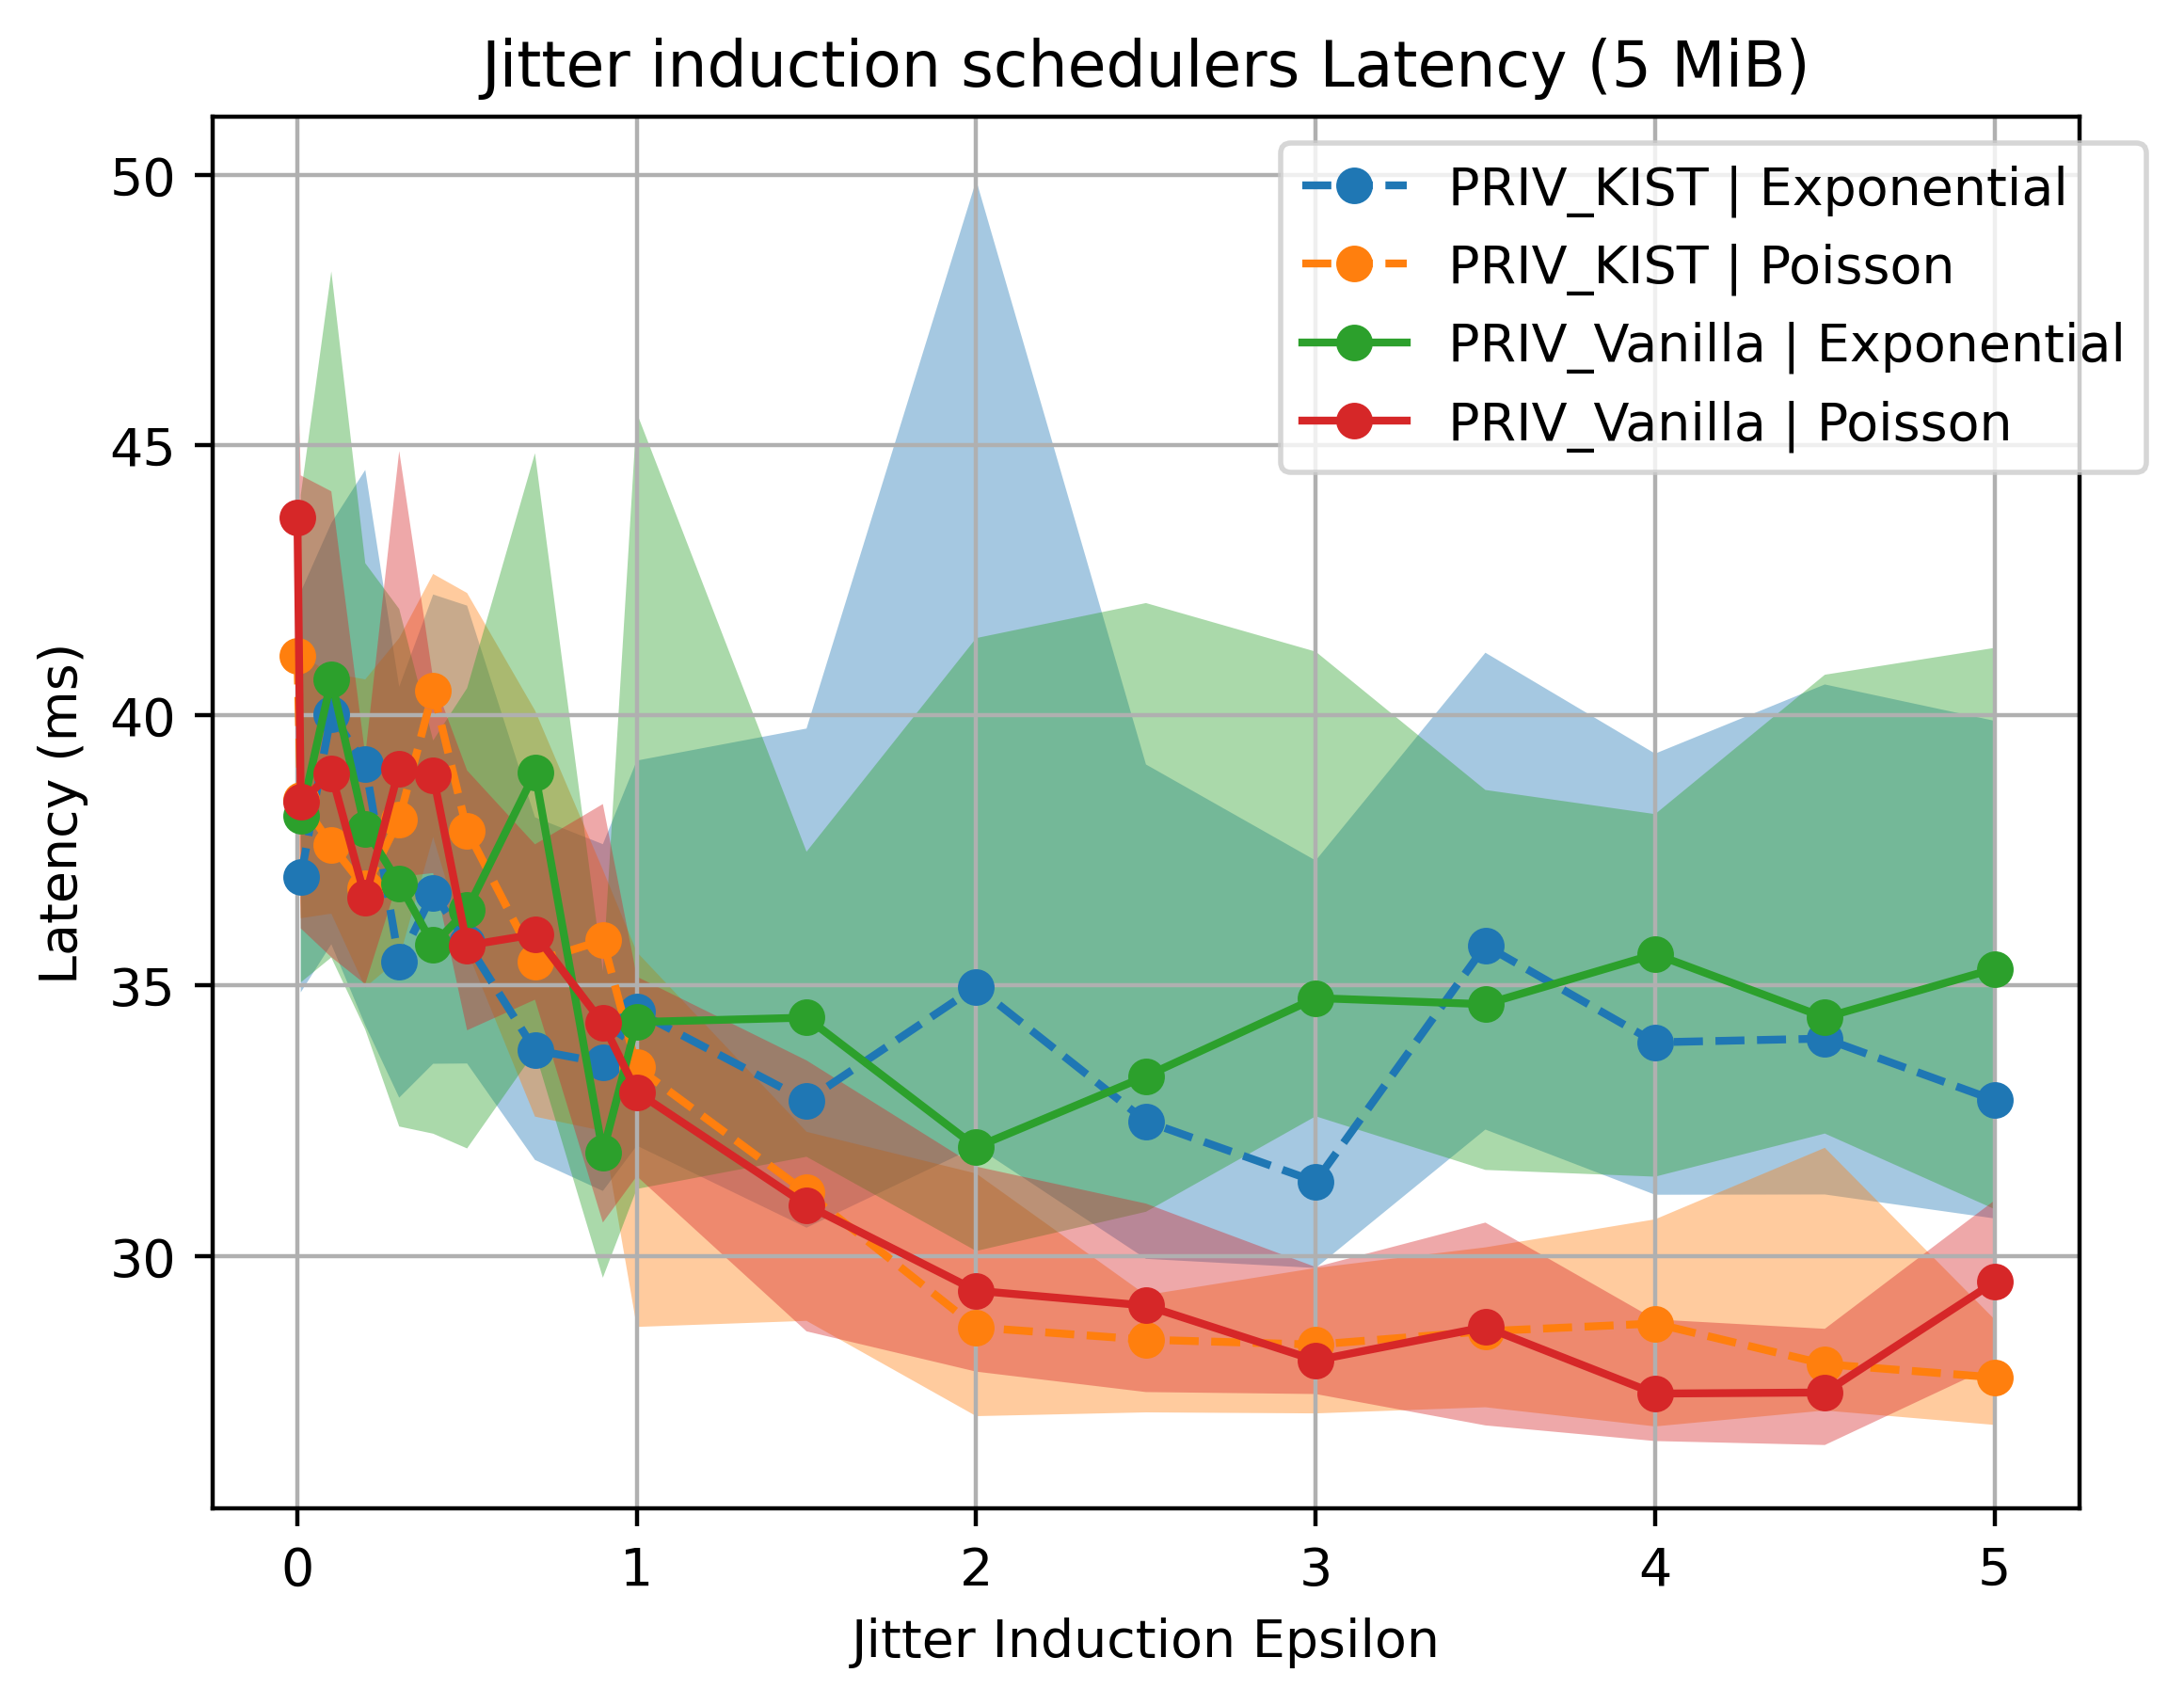
\includegraphics[width=\linewidth]{Chapters/Figures/Plots/local_latency_50_jitter_5mib.png}}
    \end{subcaptionbox}
    \vfill
    \begin{subcaptionbox}{Both Features\label{fig:local_both_latency}}[0.70\textwidth]
        {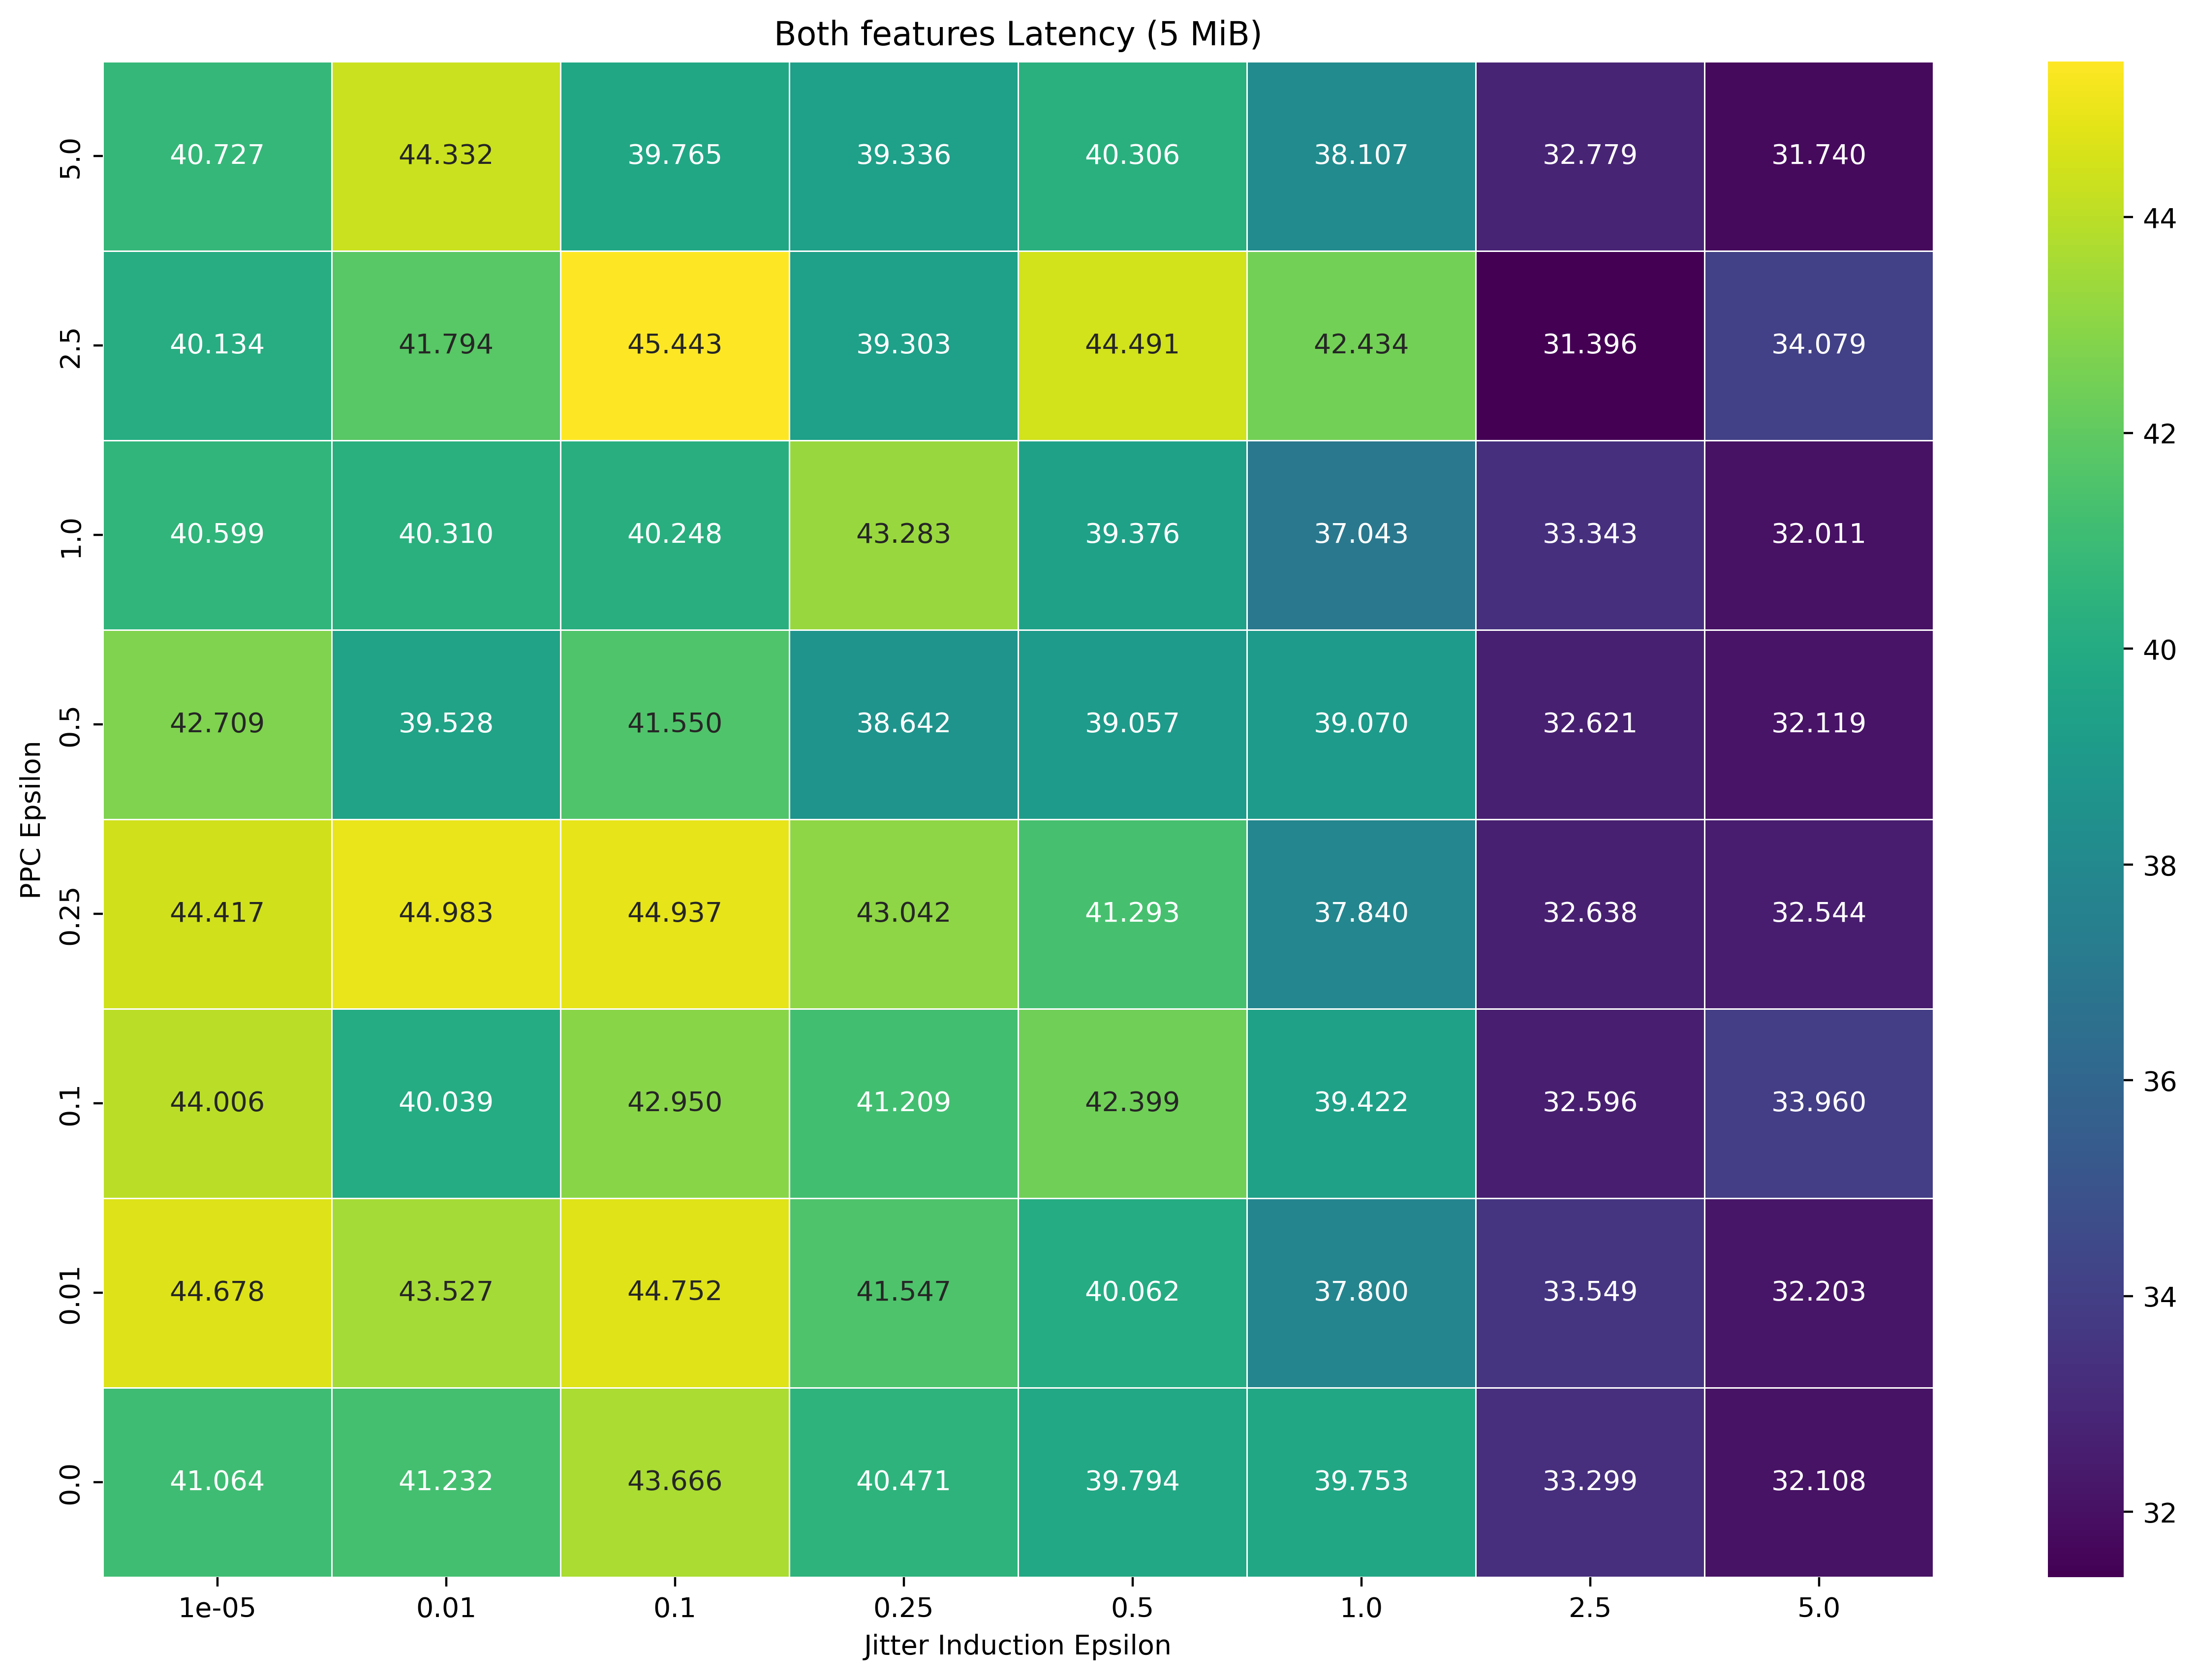
\includegraphics[width=\linewidth]{Chapters/Figures/Plots/local_latency_50_heatmap_5mib.png}}
    \end{subcaptionbox}
    \caption{Latency Results on Local Simulated Environment}\label{fig:local_latency}
\end{figure}

\begin{figure}[htbp]
    \centering
    \begin{subcaptionbox}{Only Packet Padding Cells Feature\label{fig:dist_ppc_latency}}[0.45\textwidth]
        {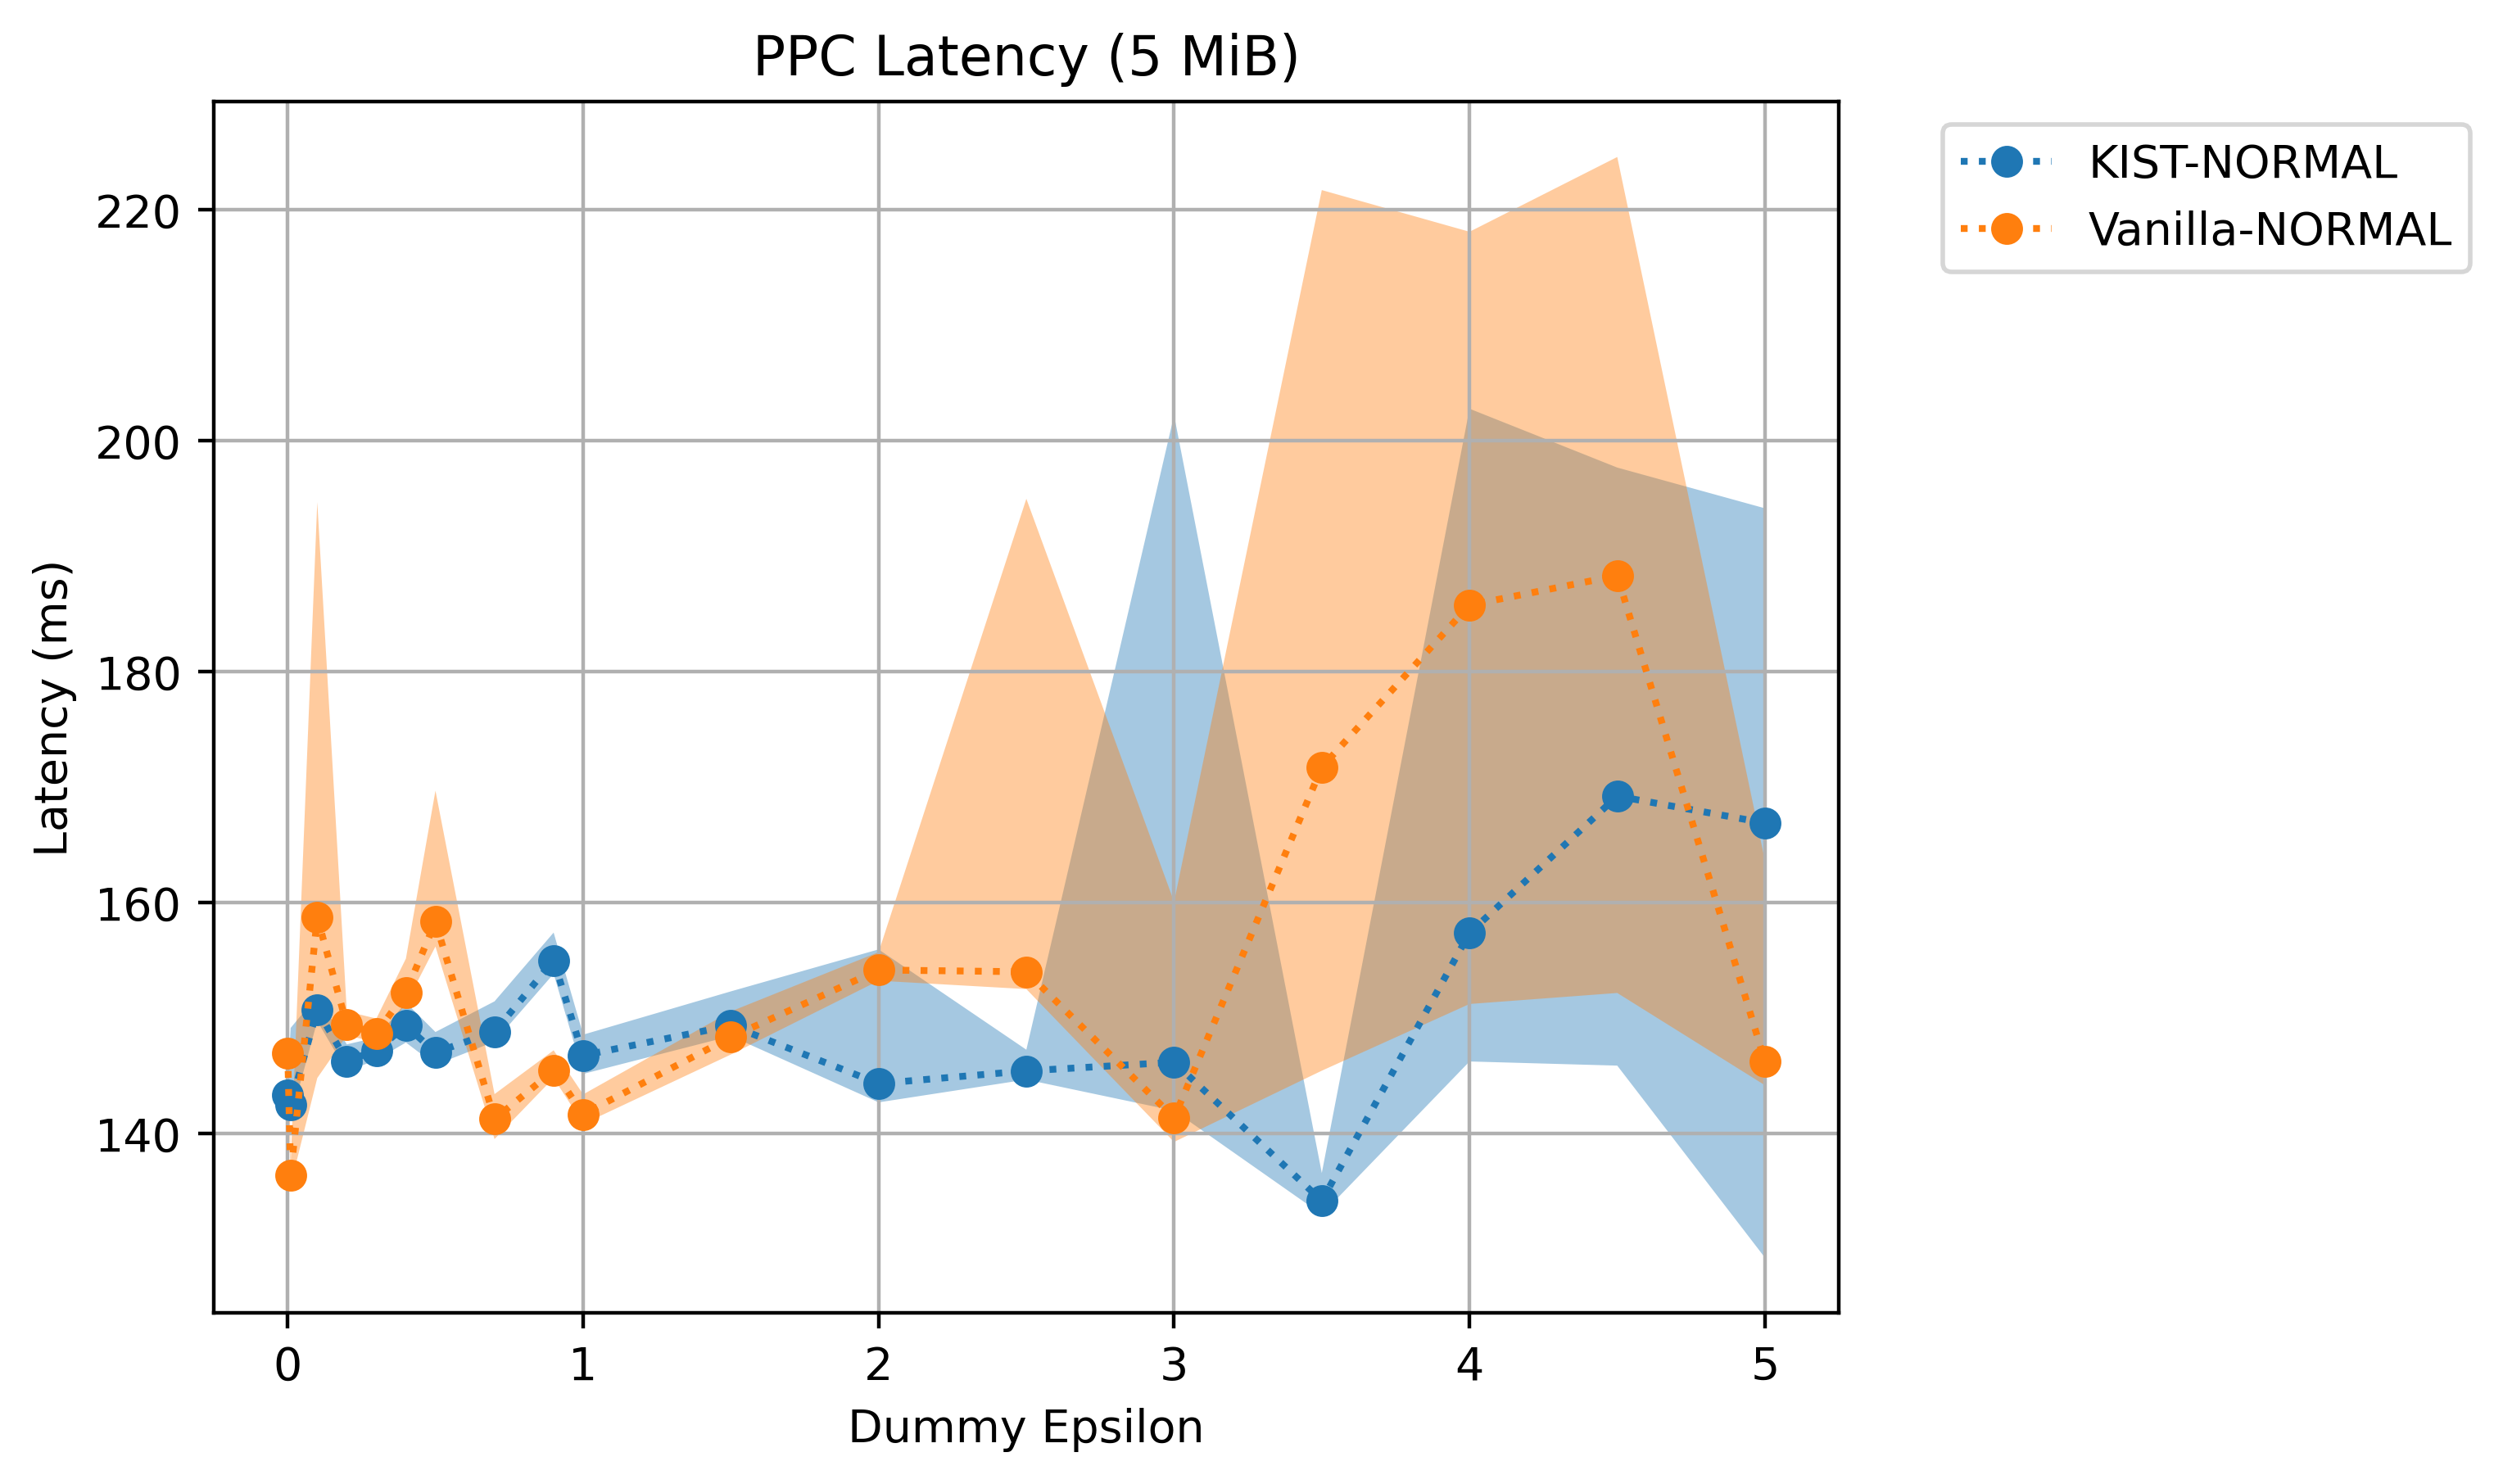
\includegraphics[width=\linewidth]{Chapters/Figures/Plots/dist_latency_50_PPC_5mib.png}}
    \end{subcaptionbox}
    \hfill
    \begin{subcaptionbox}{Only Jitter Injection Schedulers Feature\label{fig:dist_jitter_latency}}[0.45\textwidth]
        {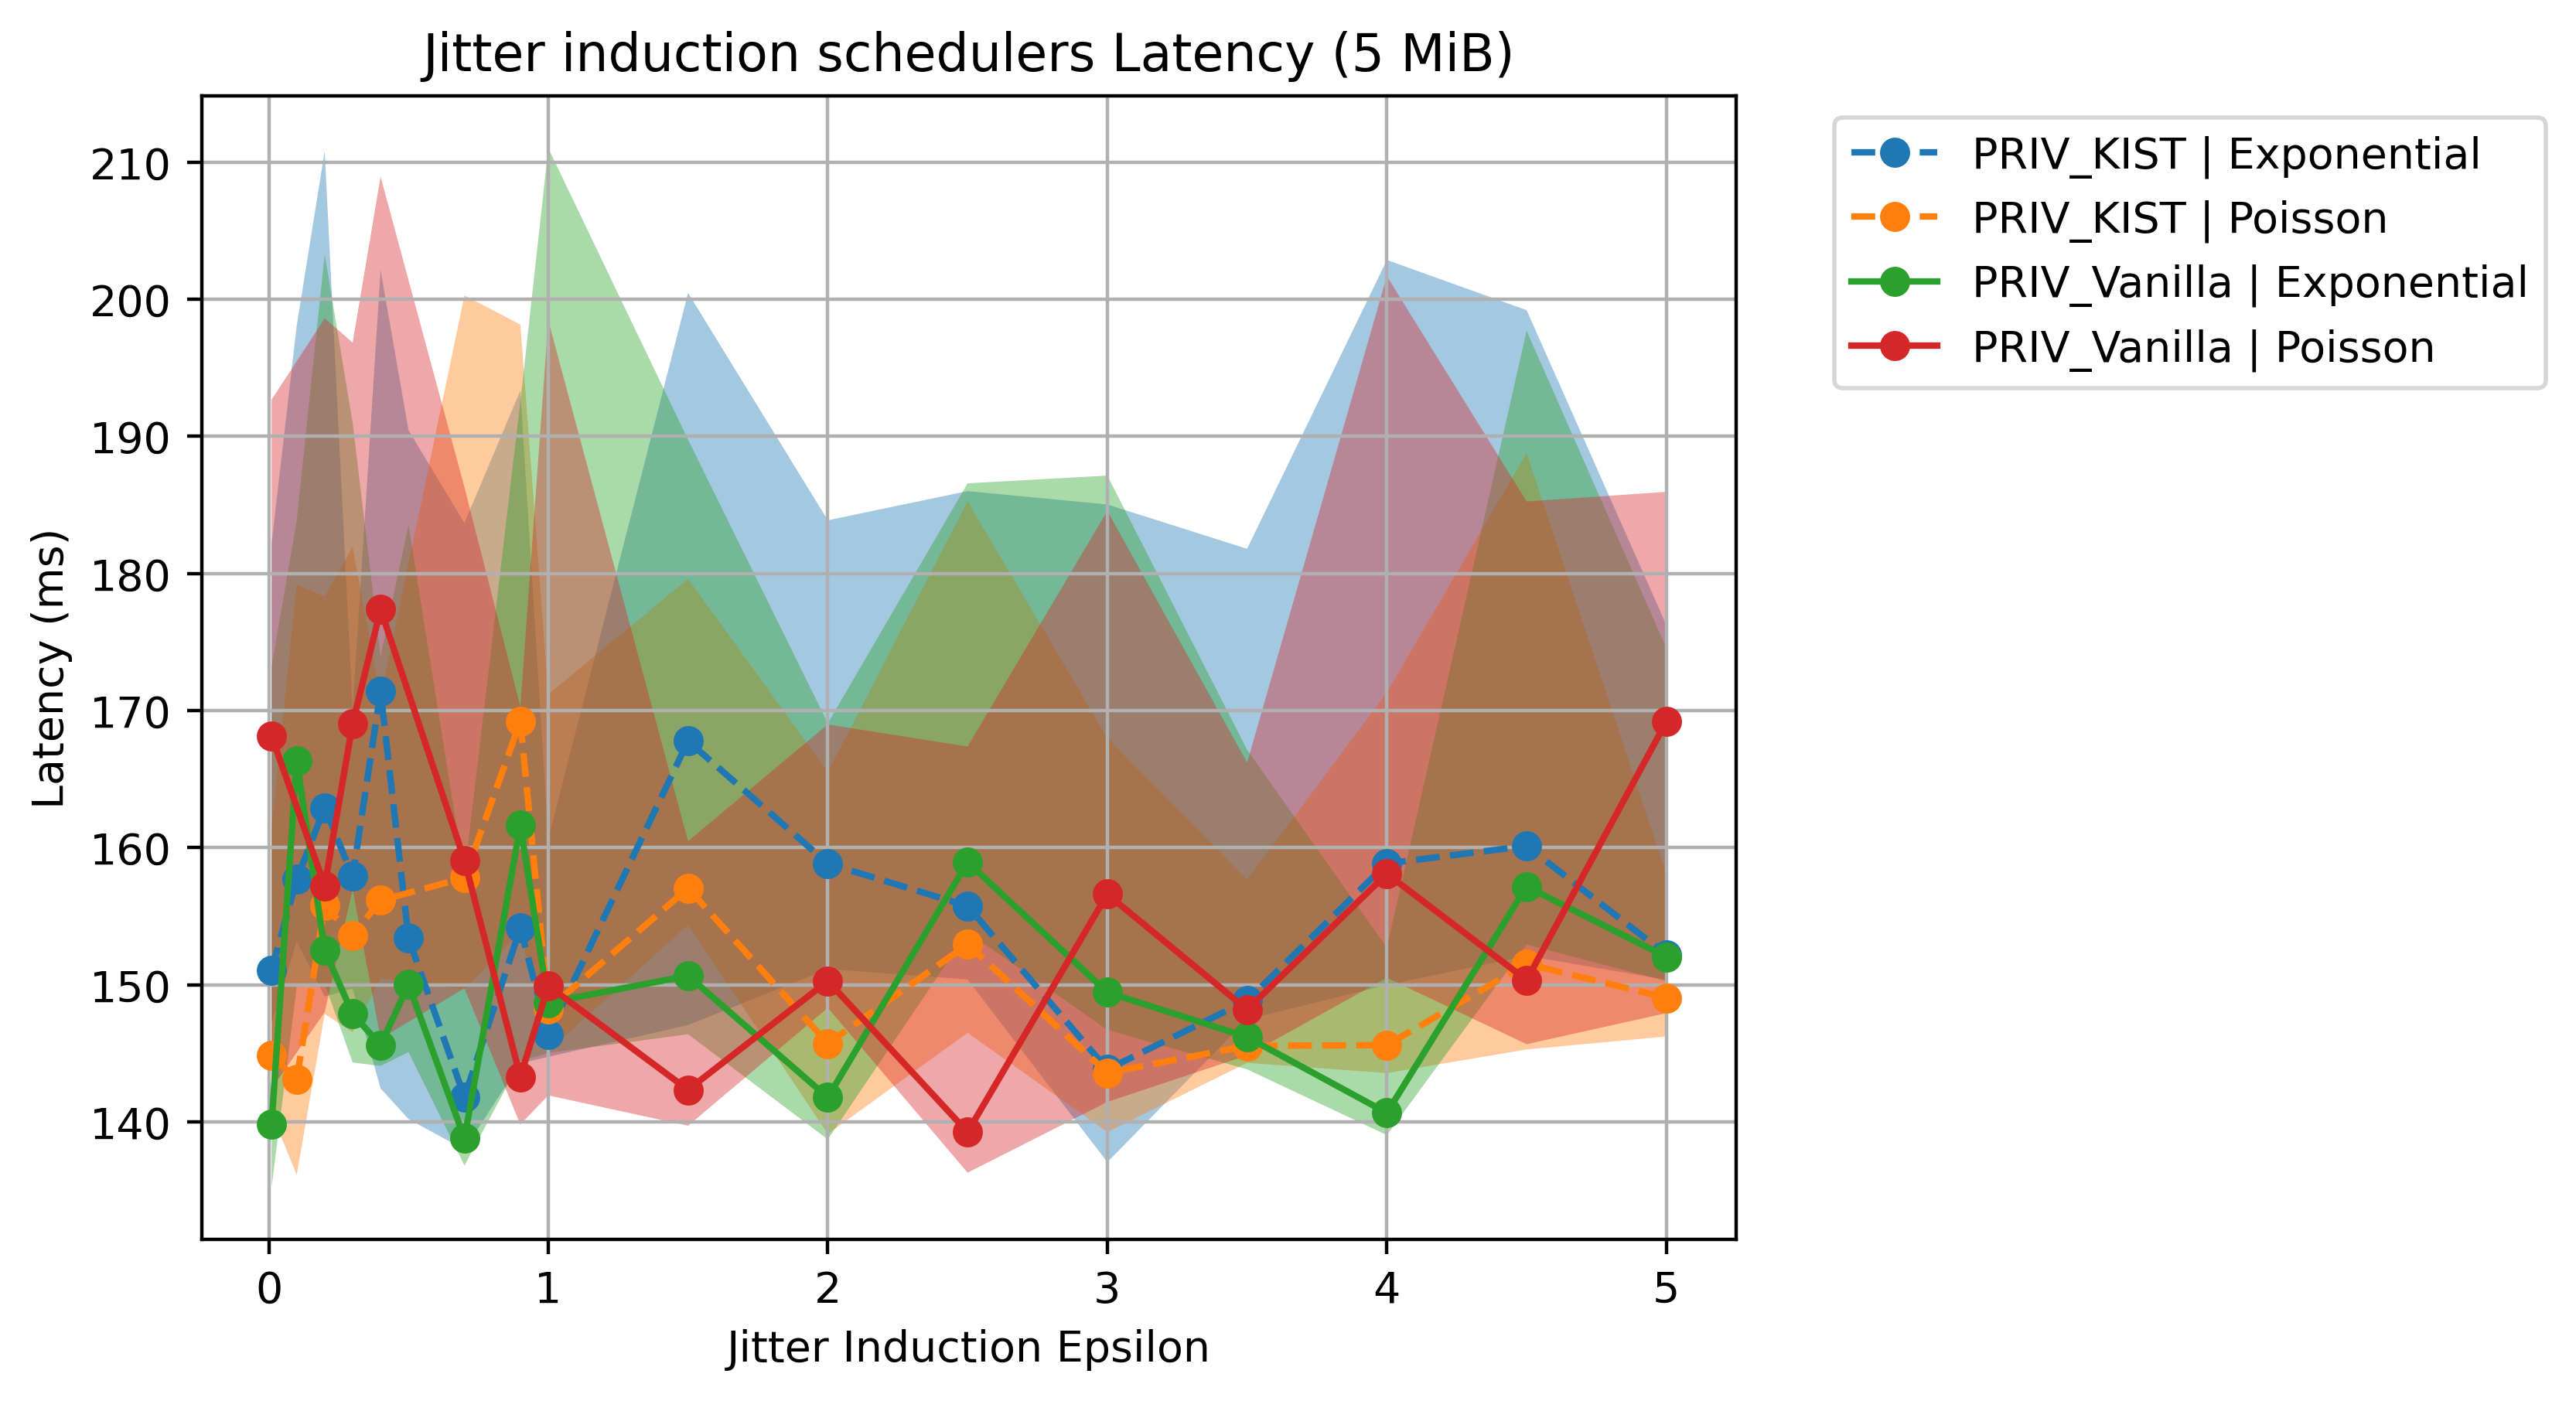
\includegraphics[width=\linewidth]{Chapters/Figures/Plots/dist_latency_50_jitter_5mib.png}}
    \end{subcaptionbox}
    \vfill
    \begin{subcaptionbox}{Both Features\label{fig:dist_both_latency}}[0.70\textwidth]
        {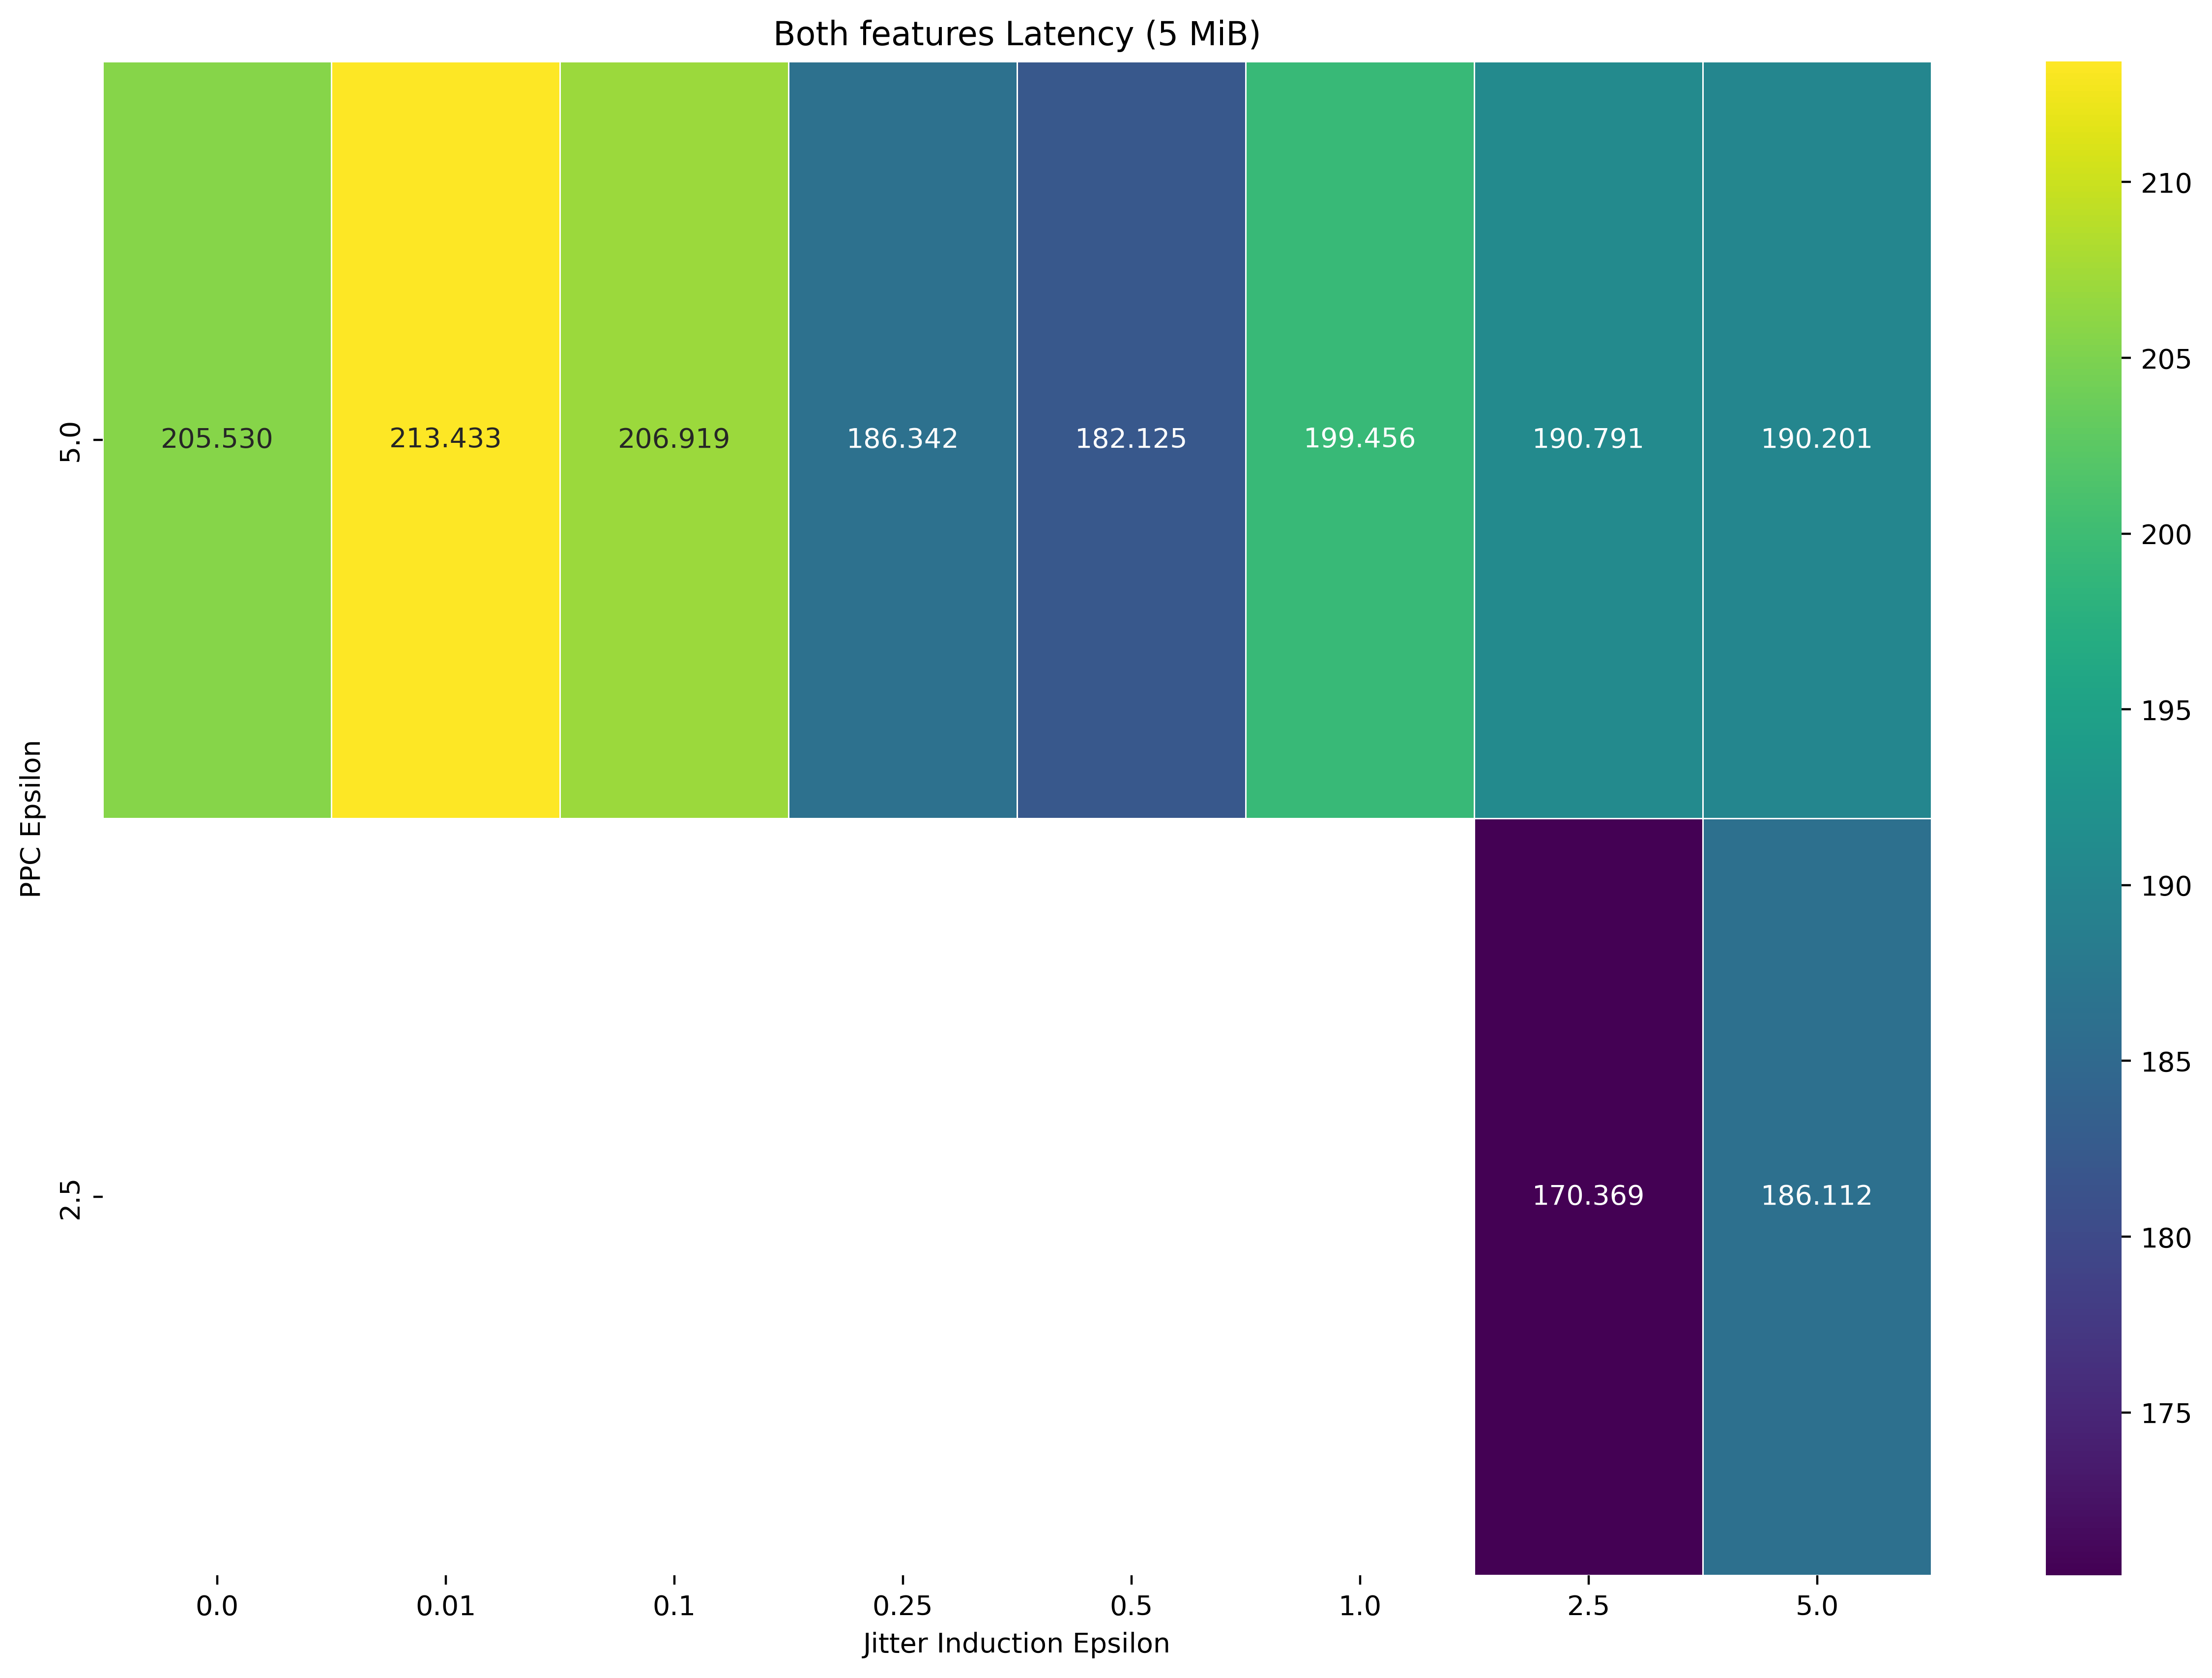
\includegraphics[width=\linewidth]{Chapters/Figures/Plots/dist_latency_50_heatmap_5mib.png}}
    \end{subcaptionbox}
    \caption{Latency Results on Distributed Environment}\label{fig:dist_latency}
\end{figure}

Unlike the previous metrics, the latency results are more sensitive to the schedulers jitter than to the PPC feature. As presented in~\autoref{fig:local_jitter_latency} and~\autoref{fig:dist_jitter_latency}, the Packet Padding Cells feature does not significantly impact the latency results, maintaining a relatively stable latency throughout the experiments. On the other hand, the Schedulers feature shows a more pronounced effect on latency, with noticeable increase when $\epsilon_{J}$ gets closer to 0, and reaching a minimum when $\epsilon_{J}$ is greater than 2. In the distributed environment, the latency results had a higher variance and a less noticeable increase in latency, as described before.
As the time of conduction this evaluation, Tor Metrics reported a median latency of 280 ms. As reported in~\autoref{tab:latency_summary}, the worse latency experience by our evaluation was 213.43 ms, with both features. This table also clearly shows that the impact of both features on latency are less apart as the impact differences produced in throughput and total time evaluations. 
%TODO: MUST TEST COMBINATIONS ON DISTRIBUTED TO GET BETTER ANALYSIS ON WORSE/BETTER TEST BENCH AND CONFIGURATION
\begin{table}[htbp]
    \centering
    \begin{tabular}{|c|c|c|}
    \hline
    \textbf{Configuration} & \textbf{Local} & \textbf{Distributed}\\
    \hline
    Tor Metrics & \multicolumn{2}{c|}{280}  \\ 
    \hline
    \multirow{2}{*}{Control} & 30.59 & 181.36 \\ 
    & 30.53 & 192.54\\
    \hline
    Only PPC & 27.45 – 33.03 & 134.16 – 188.30\\
    \hline
    Only Jitter & 27.45 – 40.66 & 138.81 – 181.95 \\
    \hline
    PPC \& Jitter & 31.40 – 45.44 & 170.37 – 213.43\\
    \hline
    \end{tabular}
    \caption{Latency Results Summary (ms)}\label{tab:latency_summary}
\end{table}

\FloatBarrier
\subsection{TLS Packets and Cells Analysis}

Finally, we present the results of our analysis on the number of false cells, the ratio of false cells, and the total number of TLS packets. These results are not directly comparable to the previous metrics, nor are addressed by Tor Metrics, but we consider relevant to demonstrate and validate the Packet Padding Cells generation and its direct influence in traffic shaping.

\begin{figure}[htbp]
    \centering
    \begin{subcaptionbox}{Number of False Cells\label{fig:local_dummy_count}}[0.45\textwidth]
        {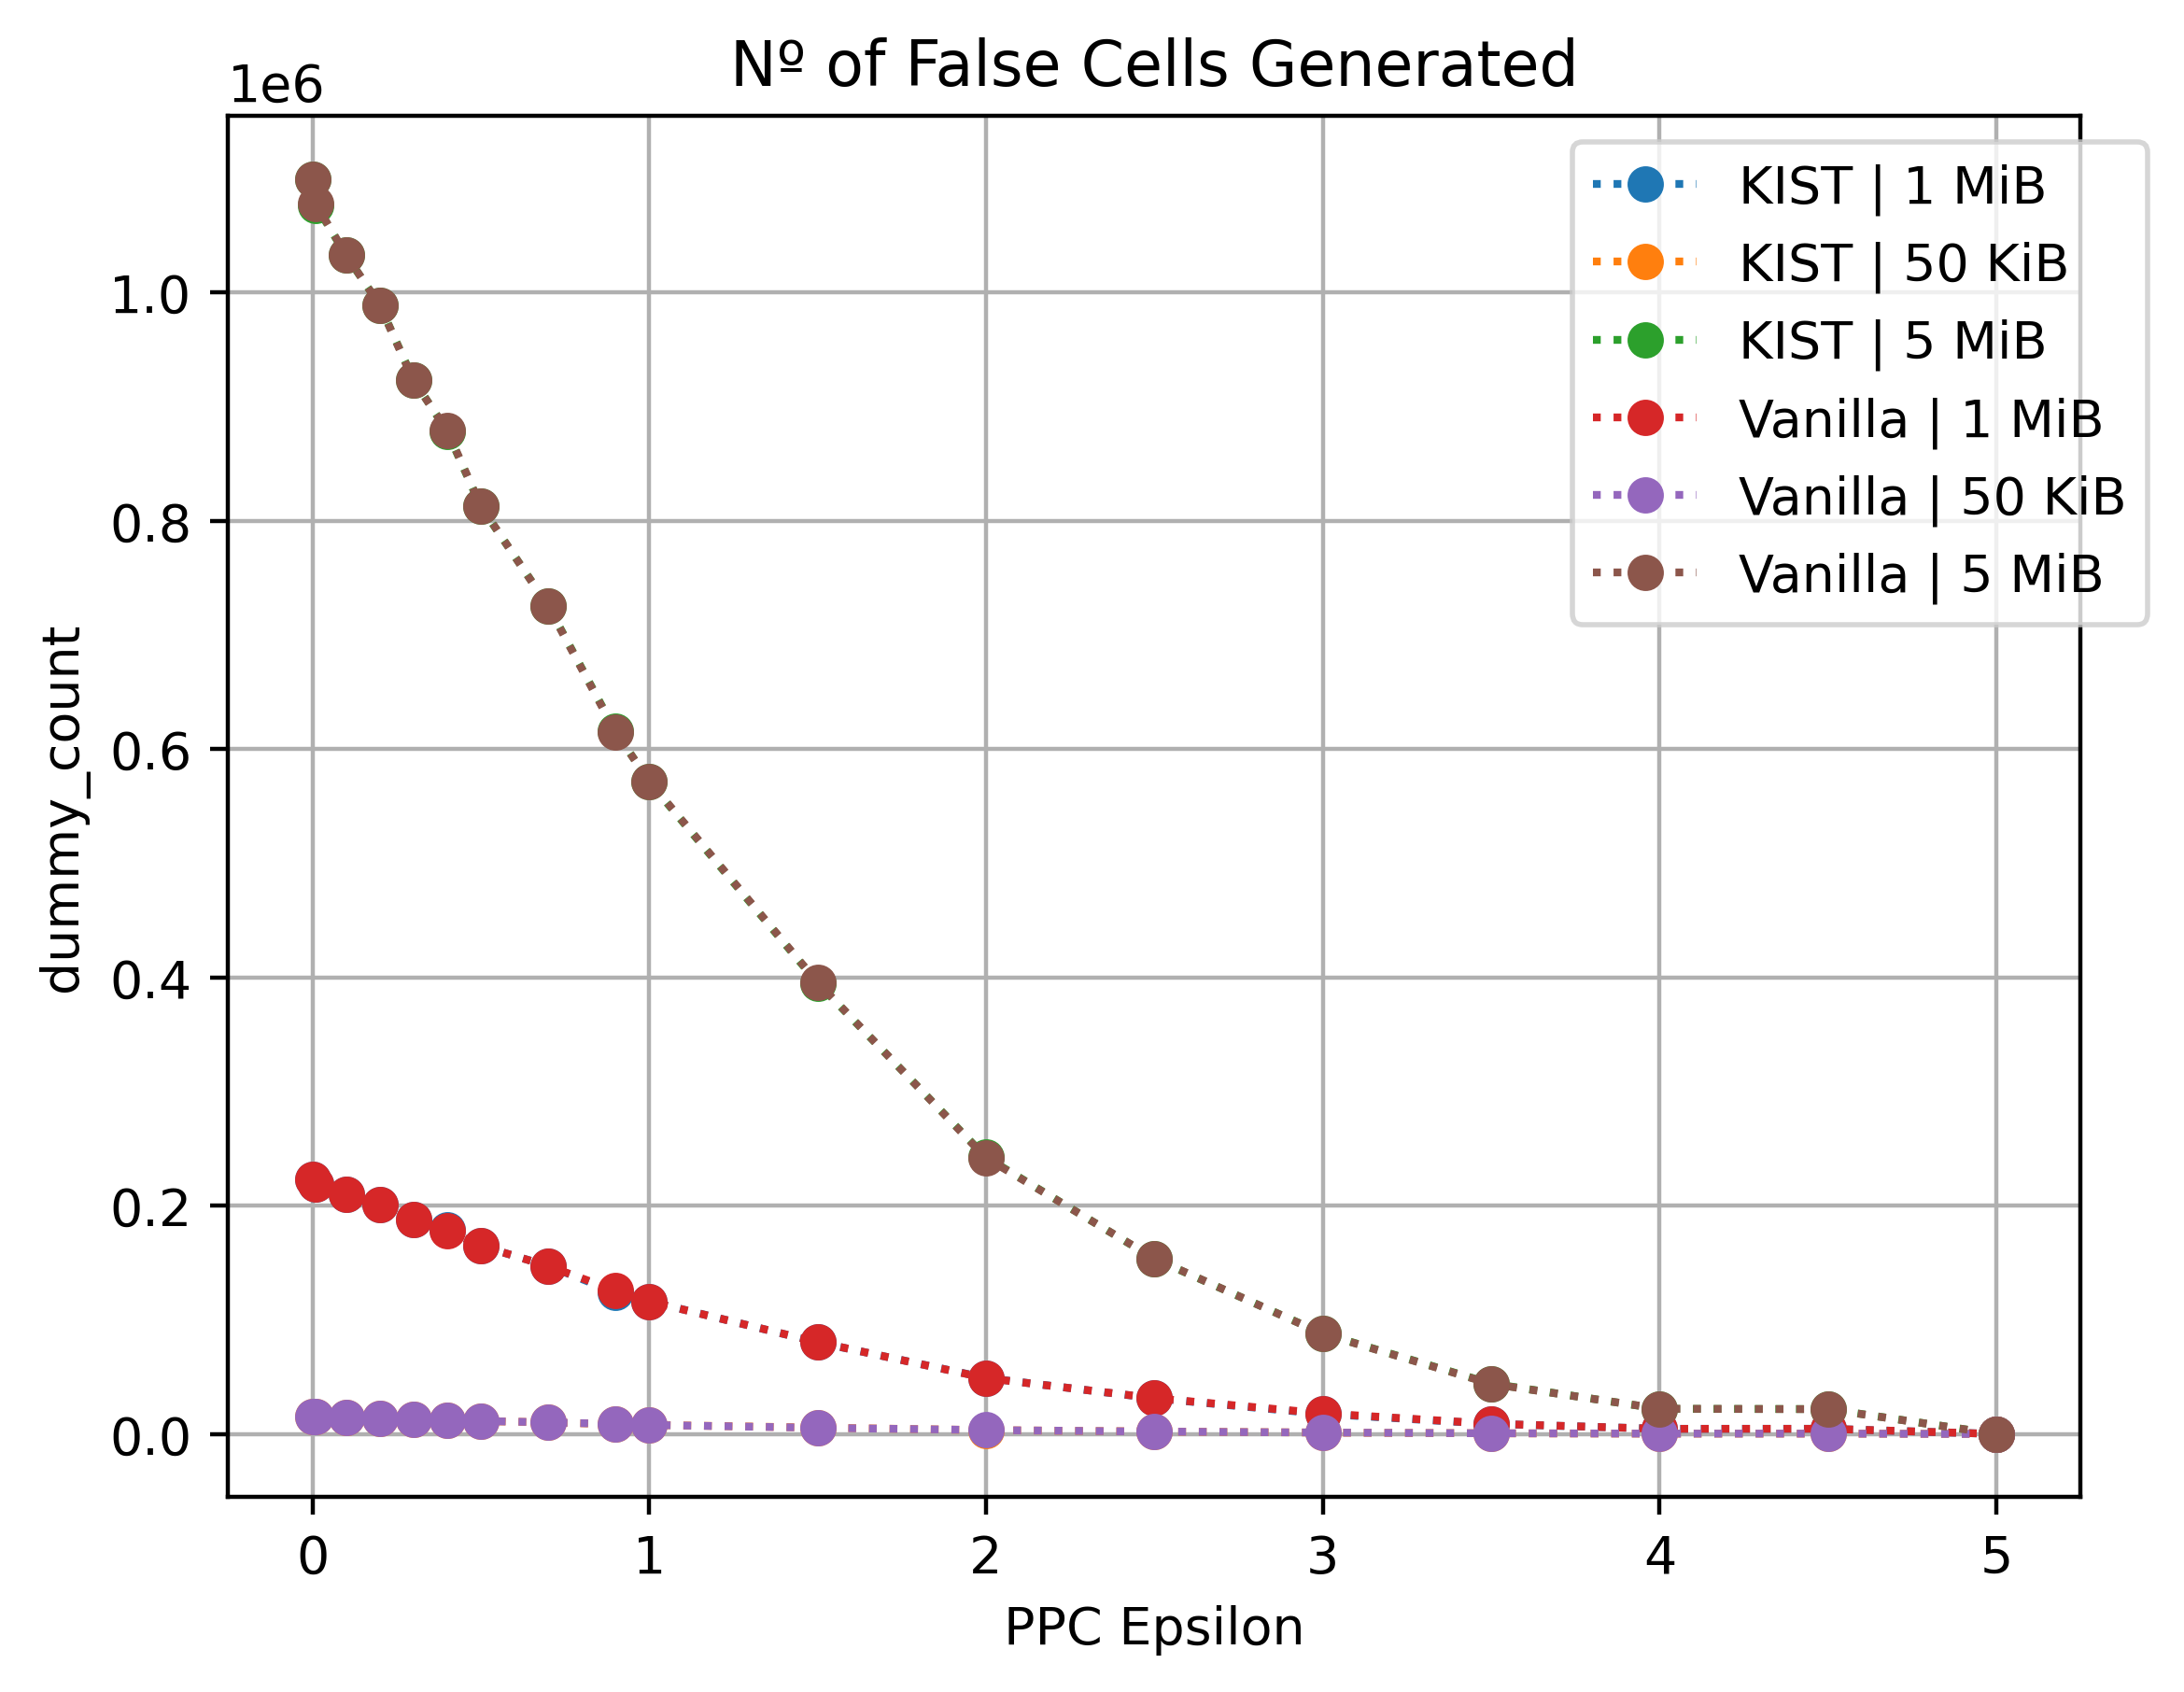
\includegraphics[width=\linewidth]{Chapters/Figures/Plots/local_PPC_count.png}}
    \end{subcaptionbox}
    \hfill
    \begin{subcaptionbox}{Ratio of False Cells\label{fig:local_dummy_ratio}}[0.45\textwidth]
        {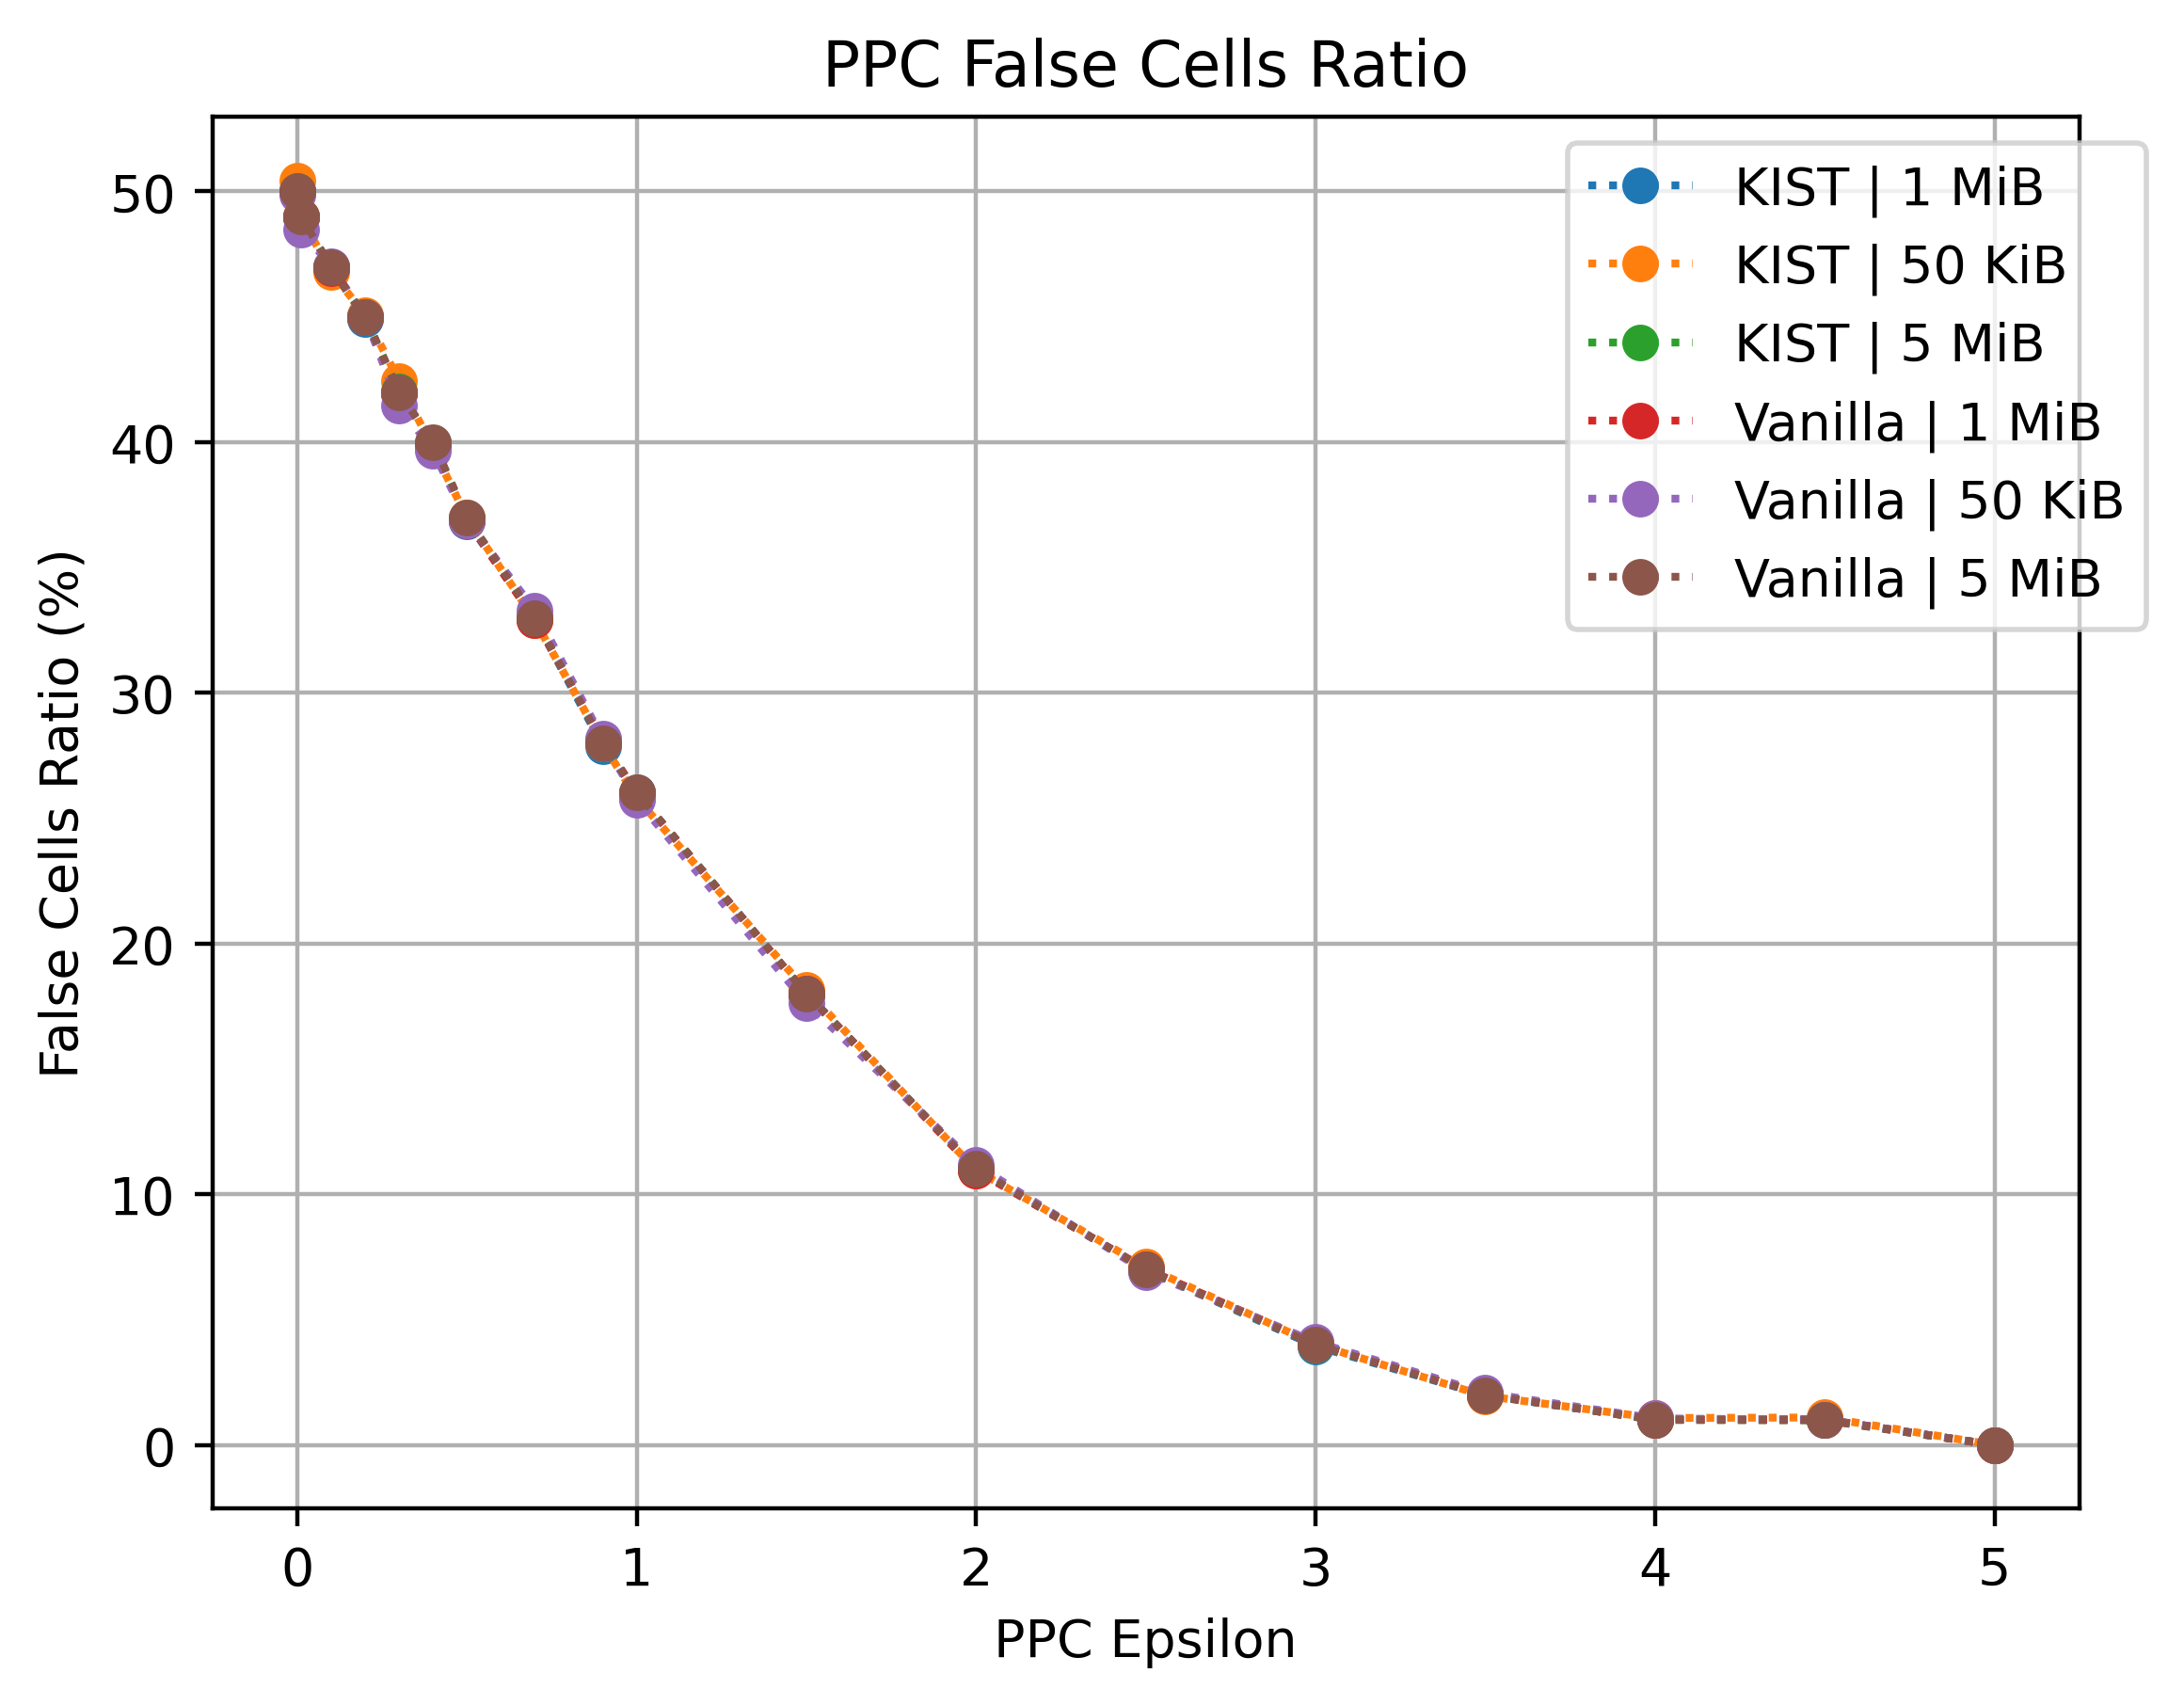
\includegraphics[width=\linewidth]{Chapters/Figures/Plots/local_PPC Ratio_5mib.png}}
    \end{subcaptionbox}
    \vfill
    \begin{subcaptionbox}{Total TLS Packets\label{fig:local_packet_count}}[0.70\textwidth]
        {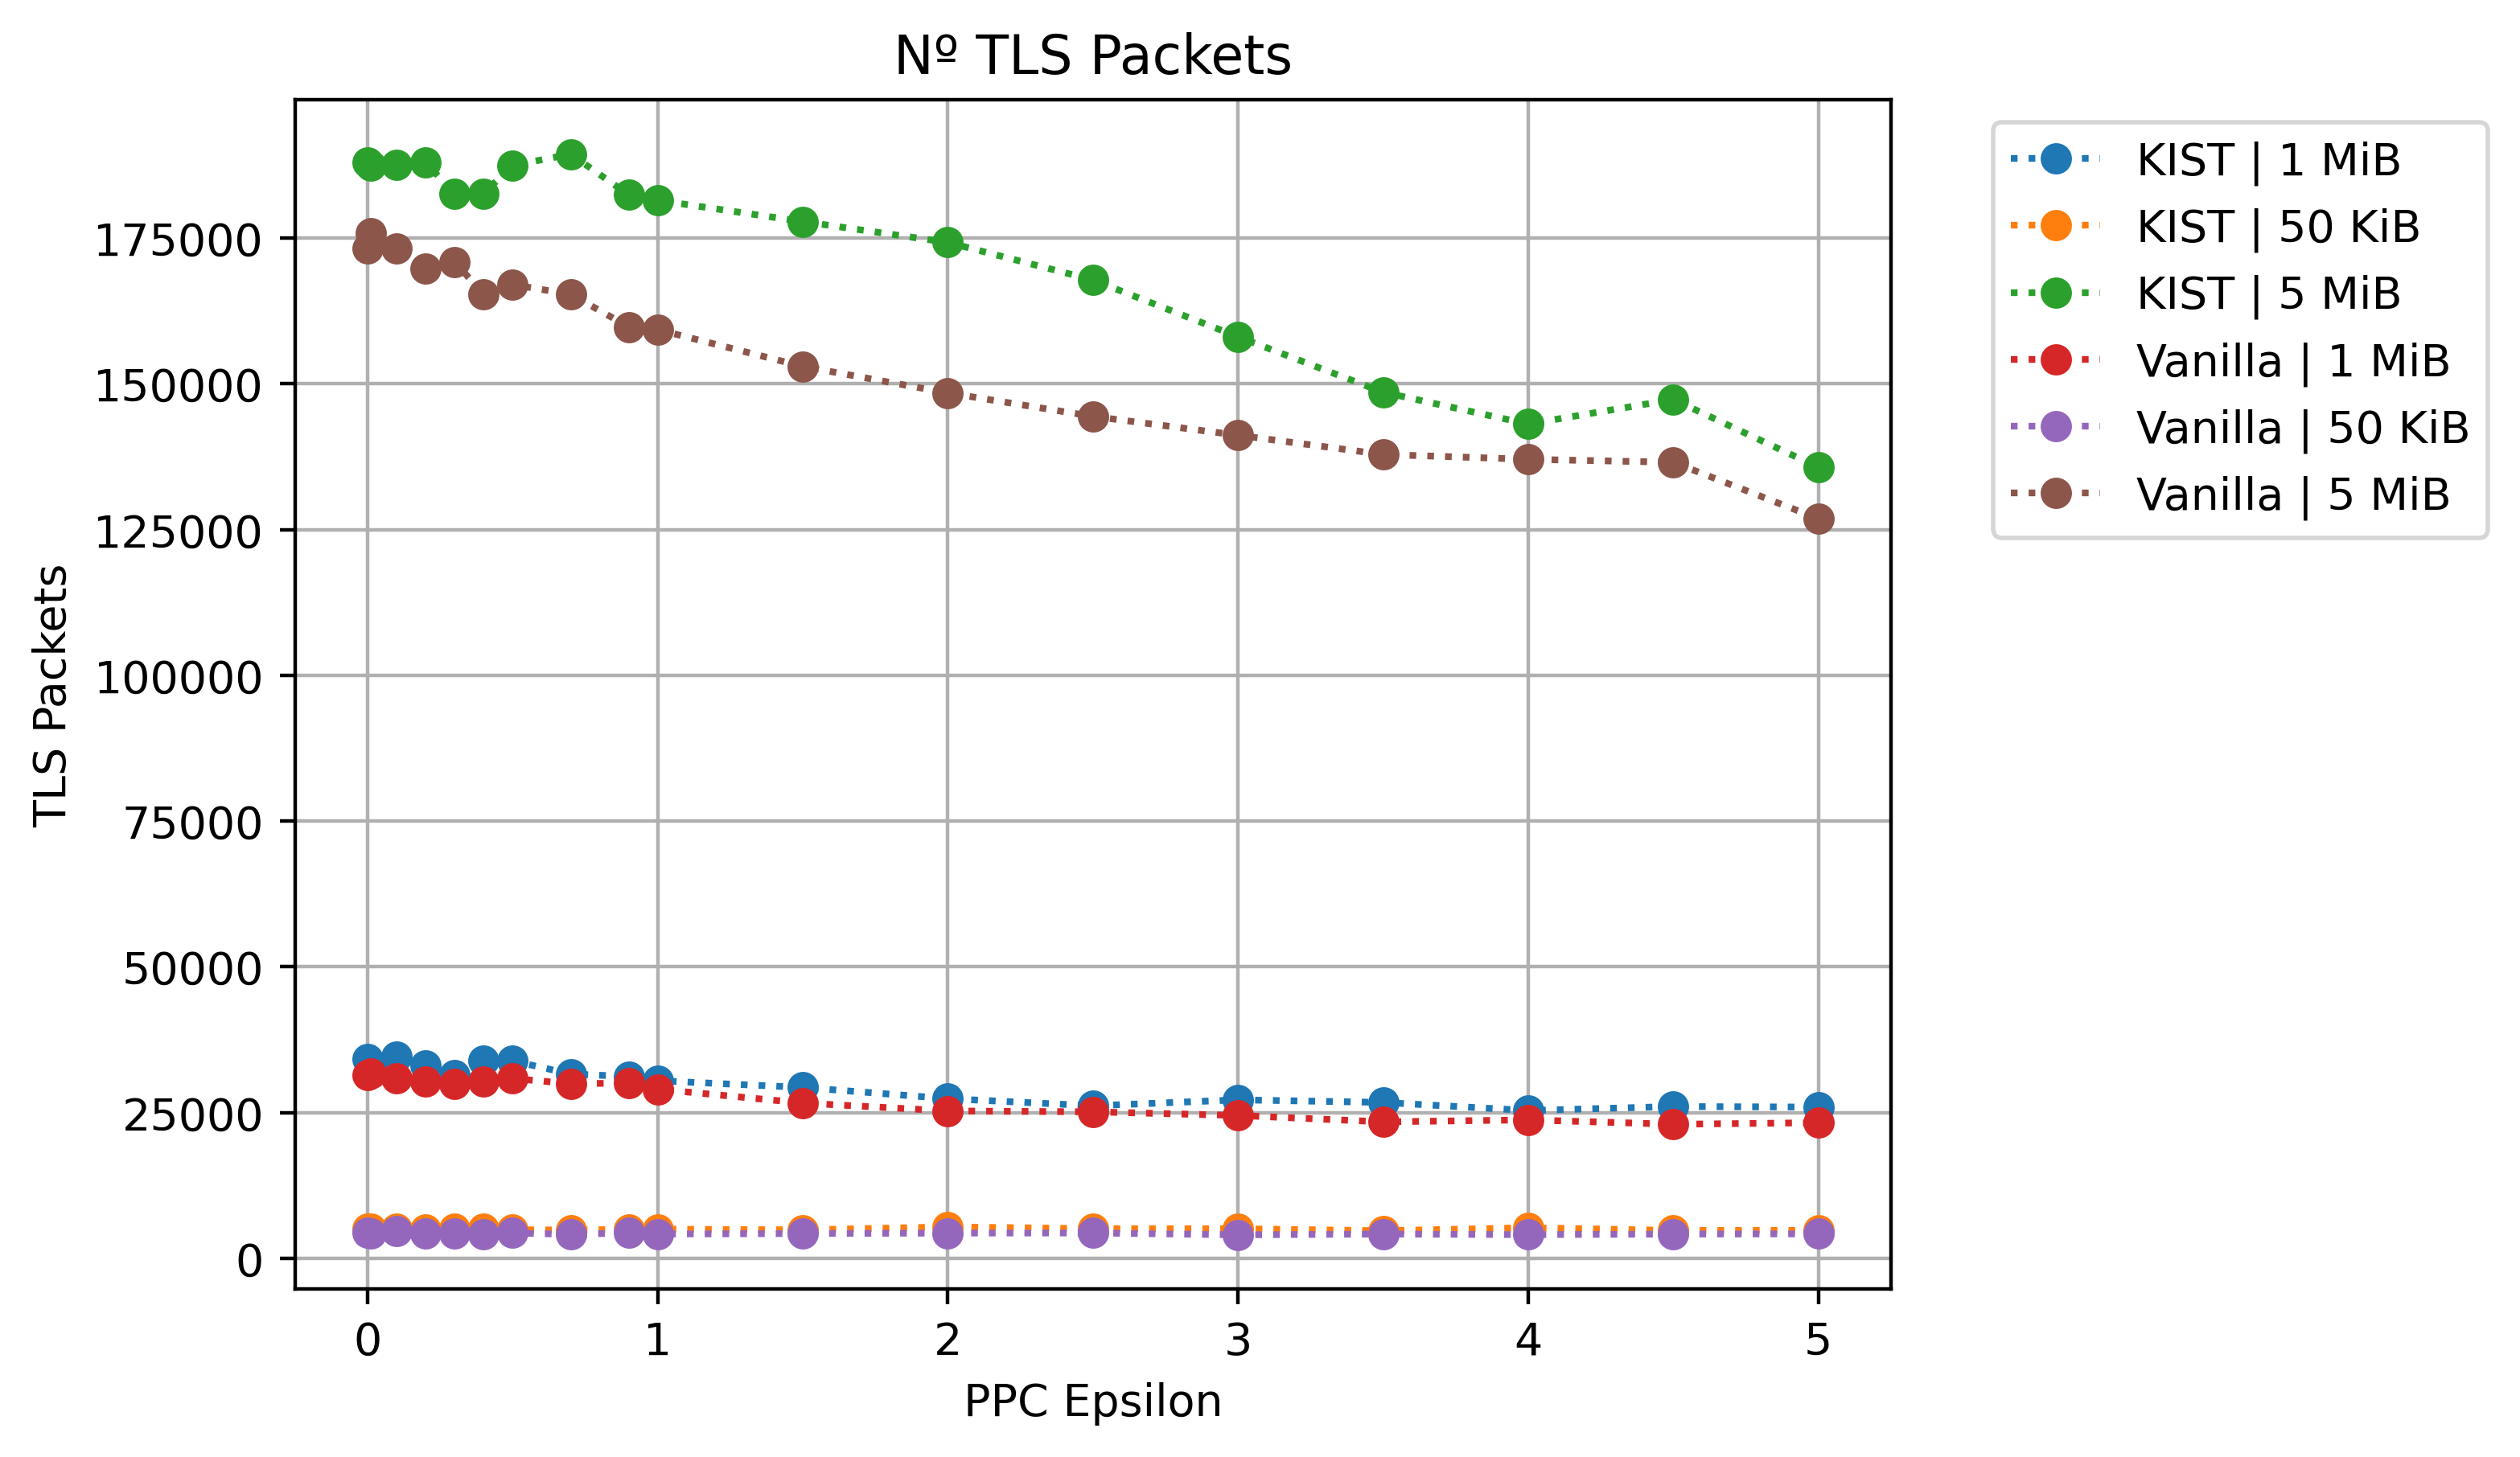
\includegraphics[width=\linewidth]{Chapters/Figures/Plots/local_packet_count_5mib.png}}
    \end{subcaptionbox}
    \caption{Cells and Packets Results}\label{fig:cell_packets_results}
\end{figure}

As expected, the number of false cells and their ratio to total cells decreases as the $\epsilon$ increases, with the highest ratio being $50\%$ when $epsilon_d = 0$. However, we observed that the total number of TLS packets does not follow a directly proportional pattern to the number of false cells, as each TLS packet can contain multiple cells, thereby adding some randomness to the traffic metadata and shape. 

\section{Unobservability Evaluation}\label{sec:unobservability_evaluation}

In this section, we evaluate the resistance of our system, focusing on the capability to withstand website fingerprinting attacks. As previously detailed in~\autoref{subsubsec:website_fingerprinting_attack}, this form of traffic analysis aims to identify the websites a user is visiting by analyzing encrypted traffic patterns to infer their online activity.
The following subsections present the methods and tools used to perform our evaluation and the experimental observations.  

\subsection{Methods and Tools}\label{subsec:methods_and_tools}

To evaluate the resistance of our system against website fingerprinting attacks, we collected traces of website accesses to be used to train and test several machine learning models. We selected 100 websites from the Tranco Top 1M website list~\cite{LePochat2019}, and sampled each website 50 times, generating 5 000 samples per test configuration. The traces were captured using \texttt{tcpdump} to generate a \textit{pcap} for each sample and for each circuit segment. The website access was simulated by executing \texttt{curl} requests to the list of websites. To perform these requests, we disabled caching to ensure that each request was treated as a new visit. The captured \textit{pcap} files recorded all packet-level network activity, such as packet size, timing, and direction, thus used to evaluate resistance to fingerprinting attacks. 

\subsubsection{Machine Learning Models}

With the before-mentioned traces and to perform the unobservability evaluation, we took inspiration in~\autocite{MIRACE} work on the evaluation of website fingerprinting attacks resistance and employed a diverse set of machine learning models used in traffic analysis research. These models include Naïve Bayes, Logistic Regression, K-Nearest Neighbors (KNN), Support Vector Machines (SVM), Random Forest, Extra Trees, Gradient Boosting, and XGBoost. These models were trained and tested using their default configurations without performing hyperparameter tuning to ensure consistency and provide a fair benchmark. They were trained using 80\% of the collected data, leaving the other 20\% for testing. Below we briefly summarize each of the used models:

\paragraph{Naïve Bayes:} A probabilistic classifier that applies Bayes' theorem and assumes a strong assumption of feature independence (naive). Its interpretability makes it a useful first step in assessing basic traffic features.
\paragraph{Logistic Regression:} A linear classification model that predicts the probability of a binary outcome based on a logistic function. It is frequently used for its simplicity and interpretability in classification tasks, especially when the data is linearly separable.
\paragraph{K-Nearest Neighbors (KNN):} A non-parametric, instance-based learning algorithm that predicts by finding the most common class among the k-nearest neighbors of a data point. It is particularly valuable when the structure of the data is unknown or highly non-linear
\paragraph{Support Vector Machines (SVM):} A robust classification algorithm that finds the optimal hyperplane to best separate data points of different classes in high-dimensional space. It excels in scenarios where data is not linearly separable by transforming input features via kernel functions.
\paragraph{Random Forest:} An ensemble learning method that builds multiple decision trees during training and outputs the class that represents the majority vote from individual trees. Random Forest reduces overfitting and improves generalization by introducing randomness in both feature selection and sample selection, and it is particularly useful for finding intricate features by capturing different patterns and variations across different labels.
\paragraph{Extra Trees:} Similar to Random Forest, but it introduces further randomness by selecting random thresholds for splitting trees, which helps reduce variance and improve predictive performance, especially in noisy datasets.
\paragraph{Gradient Boosting:} An ensemble learning method that sequentially builds models, with each new model correcting errors made by the previous ones. It is highly effective in capturing complex patterns through iterative improvements. This model helps detect nuanced traffic characteristics that may evade simpler classifiers, such as subtle variations in packet size or timings.
\paragraph{XGBoost:} An optimized version of Gradient Boosting, known for its computational efficiency and superior performance. It incorporates regularization techniques that prevent overfitting and improve model generalization, making it particularly suitable for large datasets. Its ability to model complex, non-linear patterns efficiently enables it to uncover subtle patterns.

\subsubsection{Evaluation Metrics}\label{subsubsec:evaluation_metrics}

With these models, we were able to train and test these machine learning algorithms using the collected traces, referred in~\autoref{subsec:methods_and_tools}, to evaluate the resistance of our system against website fingerprinting attacks. 
To assess the effectiveness of our system in mitigating these attacks and of each machine learning model, we extracted several evaluation metrics such as:

\paragraph{Accuracy:} Accuracy measures the ratio of correct predictions, True Positives (TP) and True Negatives (TN), to the total number of predictions, including False Positives (FP) and False Negatives (FN). This metric provides a general overview of the model's performance.  

\[ 
\text{Accuracy} = \frac{TP + TN}{TP + TN + FP + FN}
\]

\paragraph{Precision:} Precision measures the ratio of true positive to the total number of positives, important to understand the accuracy of positive predictions and the model's ability to avoid false positives.

\[
\text{Precision} = \frac{TP}{TP + FP}
\]


\paragraph{Recall:} Recall measures the ratio of true positives to the total number of actual positives, important to understand the model's ability to identify all relevant instances and avoid false negatives.

\[
\text{Recall} = \frac{TP}{TP + FN}
\]

\paragraph{F1-Score:} The F1-Score is the harmonic mean of precision and recall, providing a balanced measure that considers both metrics. It is particularly useful when the class distribution is imbalanced.

\[
\text{F1-Score} = 2 \times \frac{\text{Precision} \times \text{Recall}}{\text{Precision} + \text{Recall}}
\]


We consider a true positive if the model correctly identifies a website, a true negative if it correctly identifies that a non-website classes, a false positive if it incorrectly identifies a website, and a false negative if it fails to identify a website. 

\subsection{Experimental Observations}\label{sec:experimental_observations_unobservability}

In this section, we present the results of our unobservability evaluation, focusing on the performance of the machine learning models in identifying websites based on the collected traces. We conducted experiments using different configurations for our system, varying the $\epsilon$ values for both the Packet Padding Cells feature and the Schedulers feature. To ease the understanding of the performance of each model and each configuration, we present the results in bar plots for each metric, contemplating 3 test scenarios: (i) \textit{Packet Padding Cells}: traces collected using a network with our prototype version with only the PPC features and with maximum generation ratio of false cells ($\epsilon_{PPC} = 0$); (ii) \textit{Jitter Induction Schedulers} similar to the previous scenario but with resort to a KIST enhanced scheduler with the Poisson distribution and maximum jitter conditions generated ()$\epsilon_{J} = 0.0001$; and (iii) \textit{Both Features}: traces collected using the minimum privacy parameter values possible for both features originating in a scenario with maximum jitter and maximum false cells' ratio. 

The first two scenarios were designed to isolate the impact of each feature on unobservability. The final scenario, which combines both features, allows for an analysis of their synergistic effects and an assessment of whether their interaction could inadvertently degrade the desired unobservability properties.
This method allows a better understanding of the impact of each feature on the resistance against website fingerprinting attacks, as well as the combined effect of both features.

\subsubsection{Accuracy}

The bar plot in~\autoref{fig:models_accuracy_comparision} presents the performance of all models under the three test scenarios. The \textit{Packet Padding Cells} feature alone presented the overall highest values, specially under the \texttt{XGBoost} model. On the other hand, the other two scenarios showed very similar results across all models, demonstrating the effectiveness of the Jitter Induction Mechanism over Tor Schedulers and that the features do not negatively impact each other when combined, even though some models achieved better accuracy on both features than only the modified scheduler. 
The most accurate models were the \texttt{XGBoost}, \texttt{Random Forest} and \texttt{Extra Trees}, with values of 0.071, 0.050 and 0.0485, respectively, on the \textit{Packet Padding Cells} scenario. These results are significantly low, indicating that the models struggled to accurately identify websites based on the collected traces. This outcome is desirable in the context of unobservability, as it suggests that the implemented features effectively obfuscate traffic patterns and hinder the ability of machine learning models to perform website fingerprinting attacks. 

\begin{figure}[!h]
  \centering
  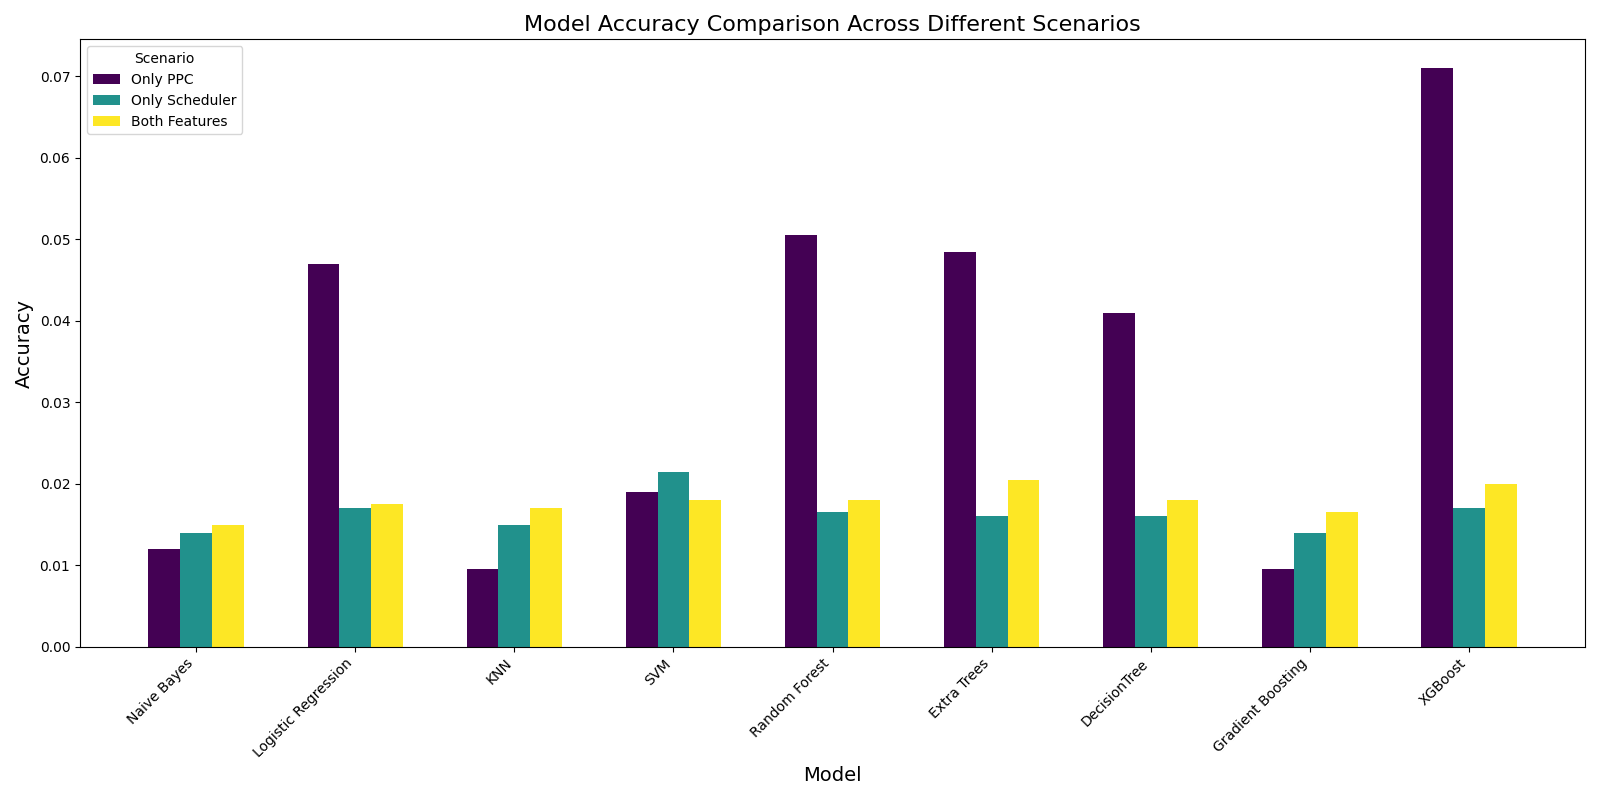
\includegraphics[width=\textwidth]{Chapters/Figures/Plots/obs-no-control/obs_Accuracy_comparison.png}
  \caption{Comparison of models' accuracy}\label{fig:models_accuracy_comparision}
\end{figure}
\FloatBarrier

\subsubsection{Precision}

The bar plot in~\autoref{fig:models_precision_comparision} shows the precision of Machine Learning models over the referred testing scenarios. The results were tightly coupled with the accuracy results, were the most accurate models correspond to the most precise, specially over the Packet Padding Cells scenario. Once again, the higher precision over this scenario proves it to be the less effective against some machine learning algorithms used. Moreover, the other scenarios show both similar and lower precision values. 
The most precise models were the \texttt{XGBoost}, \texttt{Extra Trees} and \texttt{Logistic Regression}, with values of 0.3751, 0.3202 and 0.2757, respectively, on the \textit{Packet Padding Cells} scenario. Once again these models prove to be the most effective in identifying websites, however, the precision values can be considered insufficient for a successful attack. The overall precision values are very low, indicating that the models struggle to correctly identify websites, which is a positive outcome in the context of unobservability or might suggest that the collected traces were insufficient to train the models effectively.
\begin{figure}[!h]
  \centering
  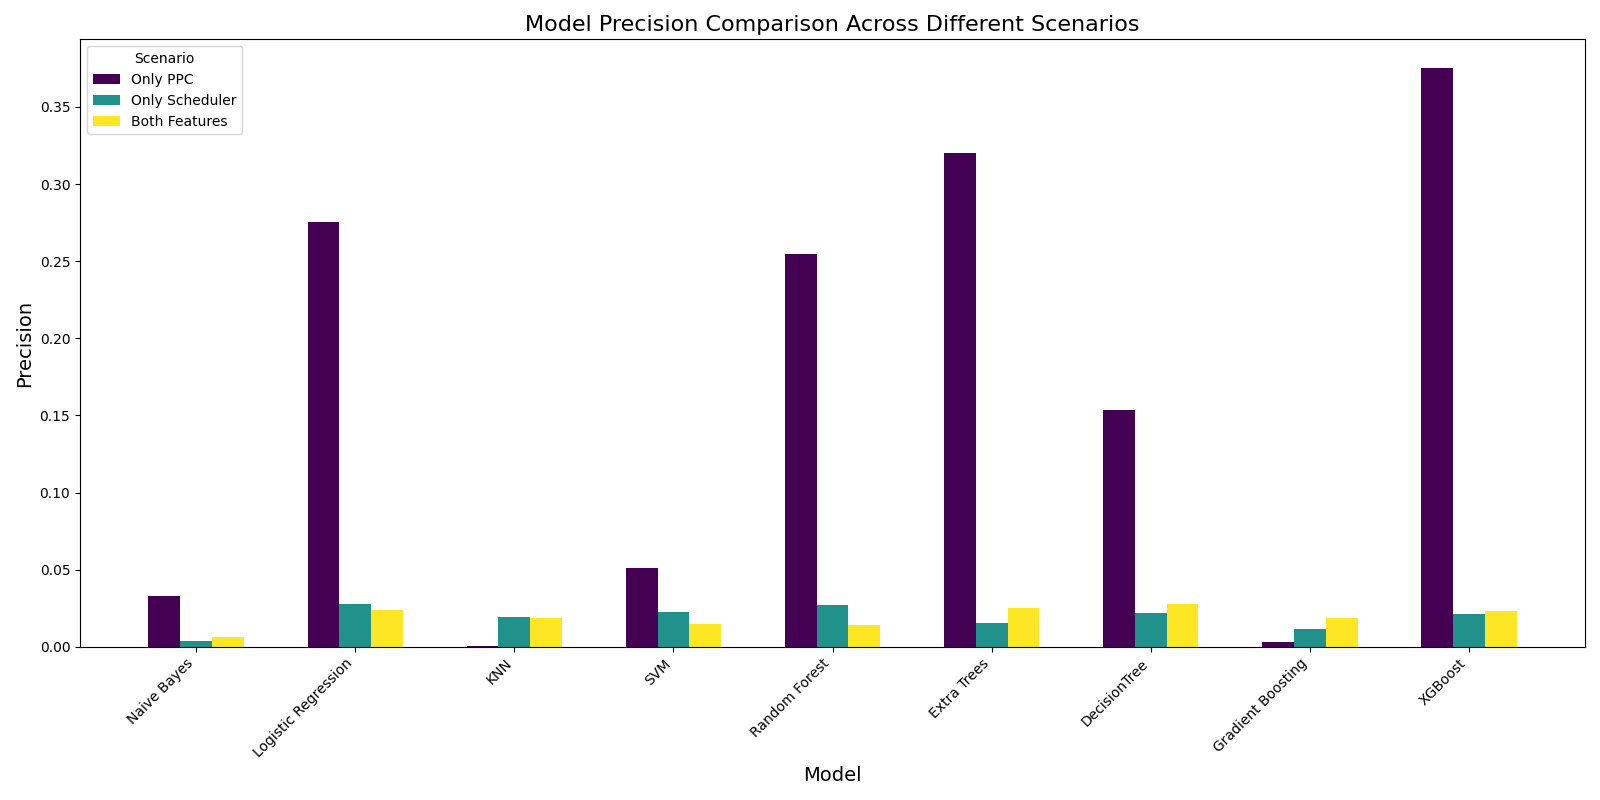
\includegraphics[width=\textwidth]{Chapters/Figures/Plots/obs-no-control/obs_Precision_comparison.png}
  \caption{Comparison of models' precision}\label{fig:models_precision_comparision}
\end{figure}
\FloatBarrier

\subsubsection{Recall}

As shown in~\autoref{fig:models_recall_comparision}, the recall results closely mirror the accuracy findings across all scenarios. This parity suggests that the models are not systematically failing to identify true positives, but rather that the overall predictive power is low, approaching the performance of random guessing. This outcome is desirable, as it indicates the absence of reliable patterns for the classifiers to exploit. Akin to accuracy, the best model is \texttt{XGBoost}, followed by \texttt{Random Forest} and \texttt{Extra Trees}, and the \textit{Packet Padding Cells} scenario proves to have the highest values of recall, with 0.0710, 0.0505 and 0.0485 for the respective mentioned models. The pattern reported in accuracy and precision is also observed in recall, where the overall values are very low, consolidating that the solution effectively mitigates the risk of website fingerprinting attacks.


\begin{figure}[!h]
  \centering
  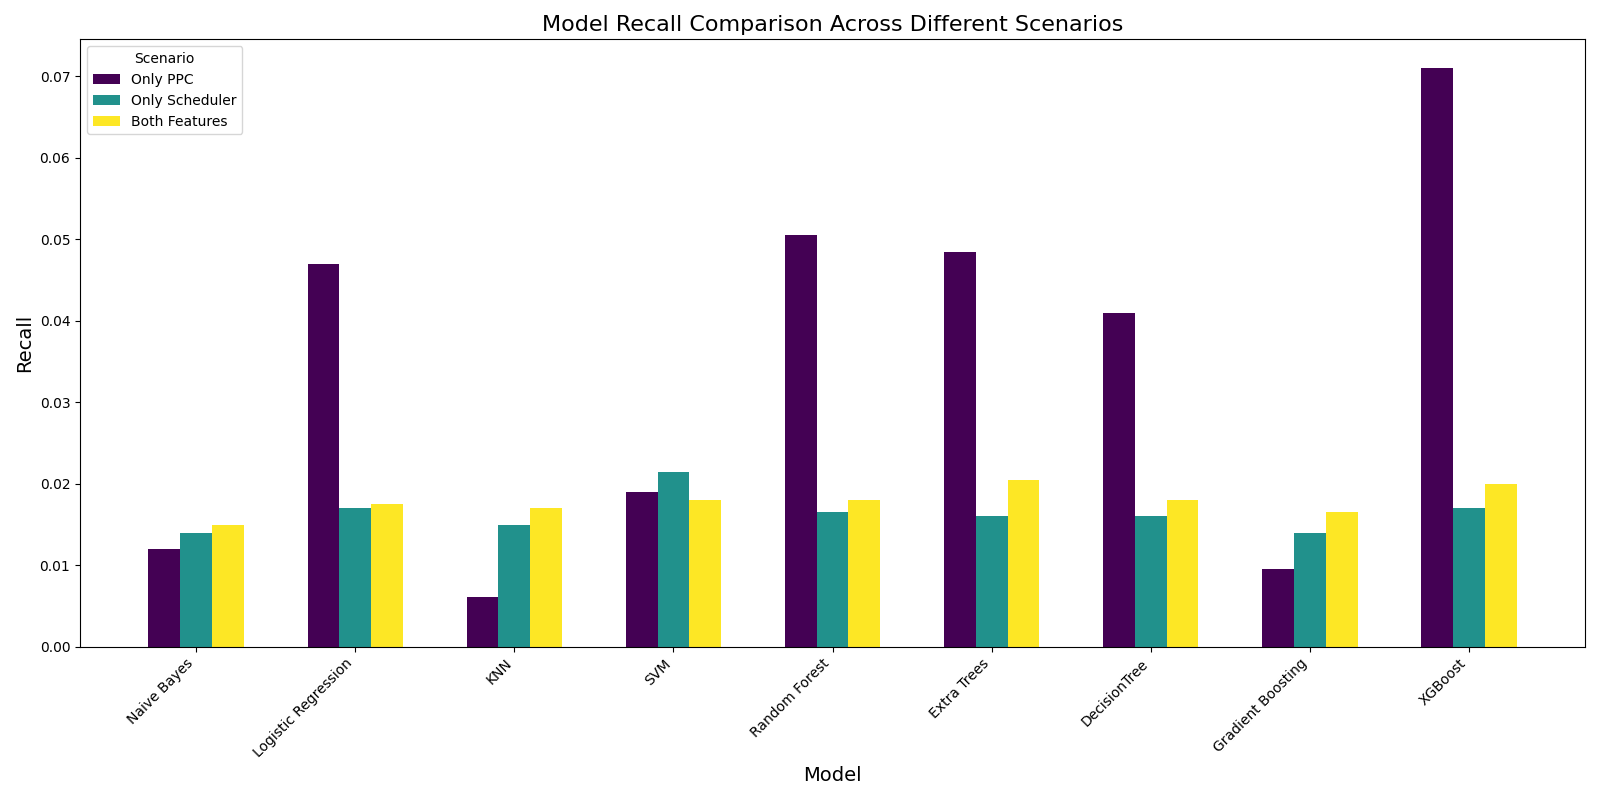
\includegraphics[width=\textwidth]{Chapters/Figures/Plots/obs-no-control/obs_Recall_comparison.png}
  \caption{Comparison of models' recall}\label{fig:models_recall_comparision}
\end{figure}
\FloatBarrier

\subsubsection{F1-Score}

Finally, the bar plot in~\autoref{fig:models_f1score_comparision} demonstrates the results of F1-Score of the experiments. As expected from the previous metrics, the  results of F1-Score follow the same pattern of all the previous metrics and validates the preceding values, indicating that the models struggle to effectively identify websites based on the collected traces. The low values observed before suggested that the F1-Score, and other derived metrics not addressed in this work, would also be low. The \textit{Packet Padding Cells} feature achieved higher values compared with the other test cases, and the \texttt{XGBoost} model again proved to be the best performant model, with a score of 0.1035, followed by \texttt{Random Forest} and \texttt{Extra Trees}, with scores of 0.0688 and 0.0679, respectively.

\begin{figure}[!h]
  \centering
  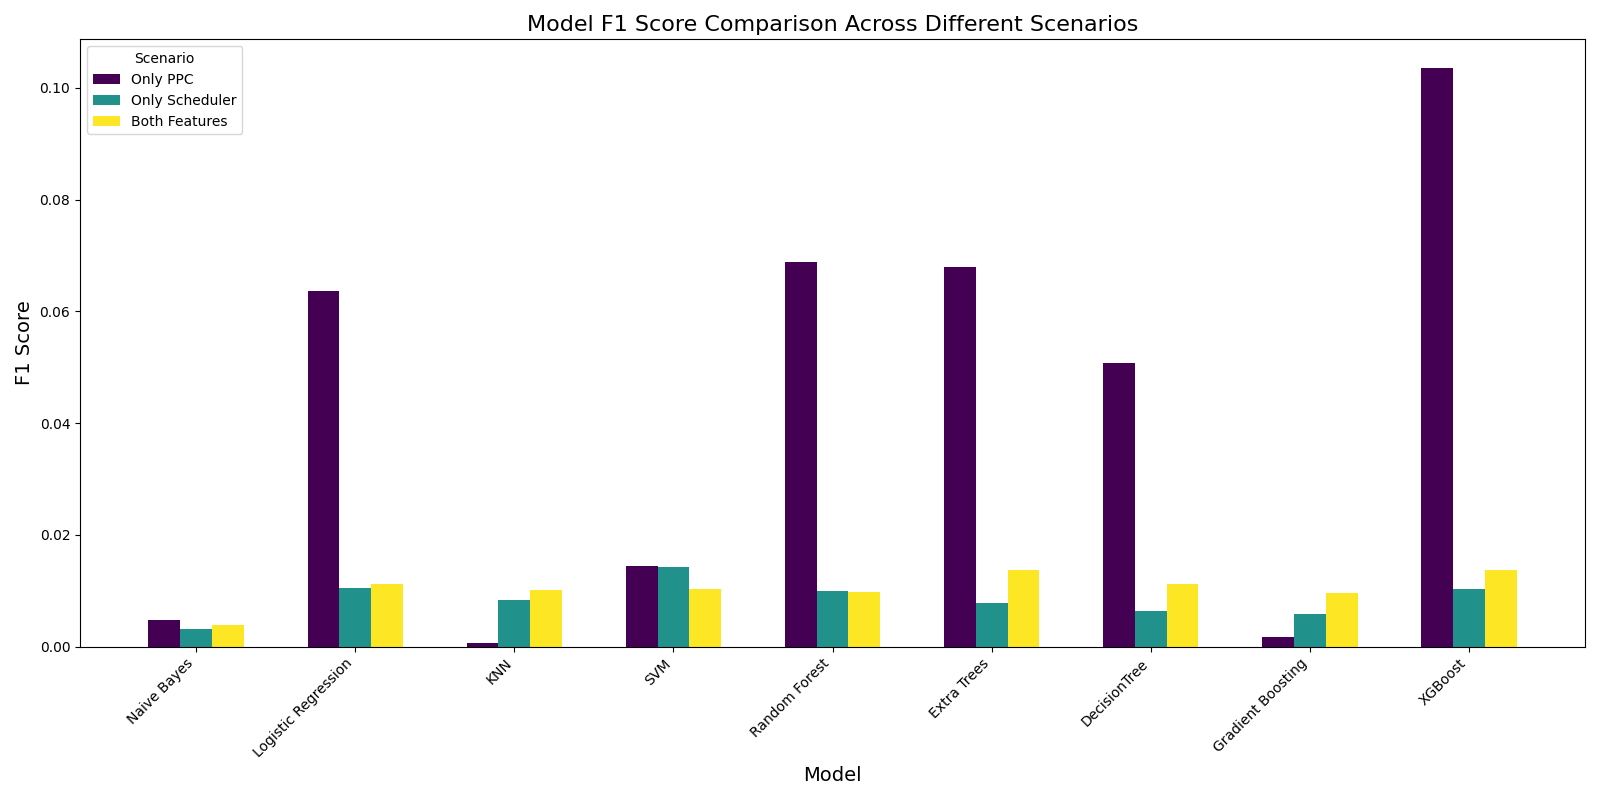
\includegraphics[width=\textwidth]{Chapters/Figures/Plots/obs-no-control/obs_F1 Score_comparison.png}
  \caption{Comparison of models' F1-Score}\label{fig:models_f1score_comparision}
\end{figure}
\FloatBarrier

In general, the results across all metrics and scenarios indicate that the machine learning models struggled to accurately identify websites based on the collected traces. The best performant model was the \texttt{XGBoost}, which achieved the highest values across all metrics, but even so, the values were significantly low. On the other hand, the \texttt{KNN}, \texttt{SVM} and \texttt{Gradient Boost} models consistently exhibited the lowest performance across all metrics and scenarios, indicating their limited effectiveness in this context. Furthermore, the \textit{Packet Padding Cells} feature consistently achieved higher values across all metrics compared to the other scenarios, suggesting that it may be less effective in obfuscating traffic patterns against certain machine learning algorithms. However, as referred before, even the highest values were significantly low, indicating that this feature was still effective in mitigating website fingerprinting attacks. The other two scenarios, \textit{Jitter Induction Schedulers} and \textit{Both Features}, showed very similar results across all models and metrics, demonstrating the effectiveness of the Jitter Induction Mechanism over Tor Schedulers and that the features do not negatively impact each other when combined.

\section{Formal Validation}\label{sec:formal_validation}

As previously mentioned in~\autoref{sec:differential_privacy}, our approach leverages Differential Privacy principles to enhance the anonymity of users within the Tor network. In this section, we provide a formal validation of our solution by redefining Differential Privacy in the context of our system and relating its theorems to our proposed mechanisms: size sets and delta sets.

An algorithm satisfies Differential Privacy if, for any two adjacent datasets (differing by a single element), the probability of any output does not change significantly when one element is added or removed. This algorithm uses a randomized function, here denoted as $F$, and its output will be similar for both datasets, with a bound defined by the privacy parameter $\epsilon$. This parameter provides a knob to tune the amount of privacy the definition provides~\cite*{DifPrivacy, DifPrivacyCalNoise, DP_Book, AlgFoundationsDP}.

Our solution introduces two key mechanisms to achieve Differential Privacy: Packet Padding Cells, which vary the size of TLS packets, and the Jitter Injection Schedulers, which vary the time intervals between TLS Packets. This way, we consider two datasets as adjacent if they differ by a single packet size or a single time interval, respectively.

The first mechanism, Packet Padding Cells, modifies the size of TLS packets by adding dummy data, which provides irreversible privacy to the TLS packets sizes, through the Post Processing property, thereby creating a set of possible packet sizes (size sets).
This mechanism is an application of the randomized response technique as described in~\autoref{subsec:local_differential_privacy}, which was inspired in an algorithm where a subject answers a sensitive question truthfully with probability $p$ and answers with a random answer otherwise, ensuring that no answer could be taken as truthfully or not, and offering Local Differential Privacy~\cite{RandomizedResponse, AlgFoundationsDP}.

By probabilistically adding dummy cells, we alter the original dataset of packet sizes. Formally, this ensures that the likelihood of observing any particular packet size is sufficiently similar regardless of whether an individual, true data packet is included in the transmission. This obfuscation provides a quantifiable privacy guarantee against adversaries attempting to infer activity from packet sizes.

More formally, for any two adjacent datasets $D$ and $D'$, and for any possible output $S$ (a specific packet size), the following condition holds:
\[P(F(D) \in S) \leq e^{\epsilon} \cdot P(F(D') \in S)\]

In this context, $F$ represents the randomized response function that adds padding to packets, which satisfies $\epsilon$-Differential Privacy. 

This feature demonstrated very interesting results in both performance and unobservability evaluations, as presented in~\autoref{sec:performance_evaluation} and~\autoref{sec:unobservability_evaluation}, respectively. The feature equipped with this randomized response mechanism showed to have no impact on the latency of the network across all the tested $\epsilon$ values, and only demonstrating an exponential increase in throughput and total time when approaching $\epsilion$ near 0. Regarding the unobservability evaluation, this feature demonstrated to be less effective obfuscating traffic patterns against machine learning algorithms, specially when compared with the results from the Jitter Injection Schedulers feature. However, the results were still very low across all metrics and models, meaning that this feature can also be considered as effective.

\begin{figure}
    \centering
    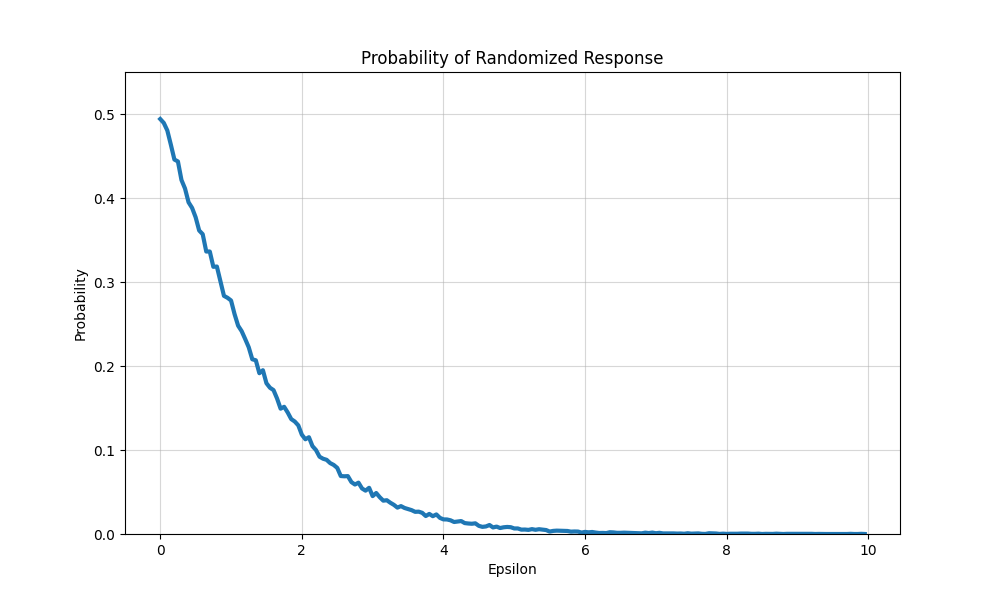
\includegraphics[width=0.7\textwidth]{Chapters/Figures/Plots/rr_stats.png}
    \caption{Probability of Randomized Response for multiple $\epsilon$}\label{fig:randomized_response_stats}
\end{figure}

The~\autoref{fig:randomized_response_stats} shows the probability of generation a false cell based on the value of $\epsilon$. As observed, the probability of generating a false cell decreases as $\epsilon$ increases, with a maximum probability of 0.5 when $\epsilon = 0$. This means that when $\epsilon$ is set to 0, there is a 50\% chance of generating a false cell, leading to the highest level of obfuscation. For $\epsilon$ values bigger than 5, the probability of generating a false cell becomes very low, approaching 0. Both this aspect and the probability distribution can be correlated with the pattern of both throughput and total time results presented in~\autoref{sec:performance_evaluation} for the Packet Padding Cells feature. To safely provide privacy, we recommend a minimum value of $\epsilon = 2.5$.

%%%%%%%%%%%%%%%%%%%%%%%%%%%%%%%%%%%%%%%%
%%%%%%%%%%%%%%%% JITTER %%%%%%%%%%%%%%%%
%%%%%%%%%%%%%%%%%%%%%%%%%%%%%%%%%%%%%%%%

The second mechanism, Jitter Injection Schedulers, introduces variability in the timing of packet transmissions by adding random delays (delta sets). This feature leverages mathematical distributions, such as~\autoref{lst:poisson_distribution} to generate differential private time intervals, ensuring that the timing of packet transmissions does not reveal information about the presence or absence of specific packets. Formally, for any two adjacent datasets $D$ and $D'$, and for any possible output $T$ (a specific time interval), the following condition holds:
\[P(F(D) \in T) \leq e^{\epsilon} \cdot P(F(D') \in T)\]

\begin{lstlisting}[language=C, caption={Poisson Distribution Pseudo-Random Number Generator implementation.}, label={lst:poisson_distribution}]
  int poisson_mechanism(double epsilon, int target, int lower, int upper)
  {
    const double lambda = (double)(upper - lower) / epsilon;

    double p = exp(-lambda);
    double sum = p;
    int k = 0;

    while (sum < uniform()) {
        k++;
        p *= lambda / k;
        sum += p;
    }

    return CLAMP(lower, target + k, upper);
  }
\end{lstlisting}

In this context, $F$ represents the randomized function that adds jitter to packet transmissions. Moreover, given $f$ as the function that givens default time interval between packets, we can define $F$ as:
\[F(D) = f(D) + \text{Poisson}(\lambda)\]
where $\text{Poisson}(\lambda)$ is a random variable drawn from a Poisson distribution with parameter $\lambda$~\cite{DP_Book, AlgFoundationsDP}. 


In the mentioned works in~\autoref{sec:differential_privacy}, it is demonstrated that mechanisms using mathematical distributions, such as Laplace, achieve $\epsilon$-Differential Privacy. In our case, we adapted the Poisson distribution to generate the random delays, which also satisfies $\epsilon$-Differential Privacy, due to issues with the Laplace distribution implementation and configuration in C. However, there are other mathematical distributions that can be used by our solution, such as the Exponential and Normal distributions.

This implementation showed very promising results in both performance and unobservability evaluations, as presented in~\autoref{sec:performance_evaluation} and~\autoref{sec:unobservability_evaluation}, respectively. On contrary to the state regarding the PPC implementation, the throughput and total time results remained significantly unaltered throughout various $\epsilon$ values, and only demonstrating an exponential increase in latency when approaching $\epsilion$ near 0. Regarding the unobservability evaluation, this feature also demonstrated to be very effective against website fingerprinting attacks, achieving very low values across all metrics and models, as presented in~\autoref{sec:unobservability_evaluation}, specially when compared with the results from the PPC feature.

\begin{figure}
    \centering
    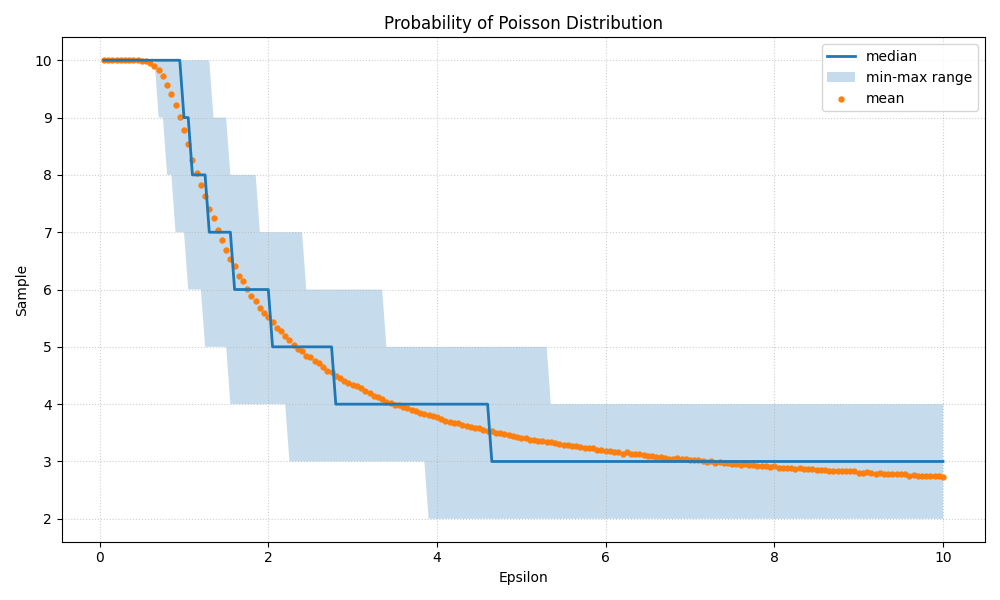
\includegraphics[width=0.7\textwidth]{Chapters/Figures/Plots/epsilon_stats.png}
    \caption{Possible samples of Poisson Distribution for multiple $\epsilon$}\label{fig:poisson_distribution}
\end{figure}

As illustrated in~\autoref{fig:poisson_distribution}, the Poisson distribution generates random delays that vary based on the value of $\epsilon$. This illustration highlights how the choice of $\epsilon$ influences the distribution of delays, with a maximum delay of 10 ms, set as a maximum in our implementation using the configurable upper bound parameter \texttt{PrivSchedulerMaxJitter}, and with a minimum of 2 ms, also set as the target parameter \texttt{PrivSchedulerTargetJitter}. It is important to note that that behavior of the jitter generation is influenced by the chosen mathematical distribution and its parameters, which can be adjusted to meet specific privacy and performance requirements. In the performed tests to understand the jitter generation behavior, we observed that the results of a not clamped Poisson distribution, with $\epsilon < 1$, could generate very high values, between 100 and 50 ms, which represent a significant delay in the context of Tor communications and in performance. To prevent this, we implemented the clamping of the generated values with the configured parameter to ensure that they remain within a reasonable range, according to the user considered maximum desired time interval and thus avoiding excessive delays. Also, this distribution becomes almost irrelevant when $\epsilon > 4$, as the generated values are very close to the target value, justifying as well the performance behavior observed in~\autoref{sec:performance_evaluation}.

Given this information, we recommend using $0 < \epsilon \leq 3$ to ensure privacy and carefully selecting the target and upper bound parameters to balance privacy and performance effectively. 

%%%%%%%%%%%%%%%%%%%%%%%%%%%%%%%%%%%%%%
%%%%%%%%%%%%%%%% BOTH %%%%%%%%%%%%%%%%
%%%%%%%%%%%%%%%%%%%%%%%%%%%%%%%%%%%%%%

Both features must be carefully used to ensure minimal privacy loss, as the total privacy cost of multiple differentially private mechanisms is the sum of their individual privacy costs, according to the Sequential Composition theorem. Therefore, if both features are applied to the same dataset, the overall privacy guarantee is given by:
\[P(F(D) \in G) \leq e^{\epsilon_1 + \epsilon_2} \cdot P(F(D') \in G)\]
where $\epsilon_1$ and $\epsilon_2$ are the privacy parameters for the Packet Padding Cells and Jitter Injection Schedulers, respectively, and $G$ is any possible output (a specific packet size and time interval)~\cite{DP_Book, AlgFoundationsDP}.
In this context, the combination of both features demonstrated to be very effective against website fingerprinting attacks, achieving very low values across all metrics and models, as presented in~\autoref{sec:unobservability_evaluation}, specially when compared with the results from the PPC feature.
These observability experimentation results also showed that the implemented Poisson distribution for injecting jitter into the Tor Schedulers was more effective than the random response mechanism used for generating Packet Padding Cells, and that their combination did not reduce their individual effectiveness.
Moreover, the performance evaluation demonstrated that the combination of both features also combined the performance impact of both features. 

\section{Summary}\label{sec:validation_summary} %1pager

% Resume what was presented and done in this chapter
This chapter presented a comprehensive experimental validation and evaluation of the TTT prototype, focusing on its performance and unobservability under various configurations and conditions, and on the formal validation of the Differential Privacy guarantees provided by the prototype. Our analysis unrevealed significant insights over the extension of Tor source code and the impact of both jitter injection and packet padding based on Differential Privacy over both performance and unobservability, as well as the software privacy guarantees provided to users. 
% Resume Performance Results

To test the performance of both implemented features, we run several tests with variable values of $\epsilon$ and mathematical distributions, collecting the latency, throughput and total time of each measurement. Furthermore, we also collected data over the number of false cells generated, the ratio of these cells compared to the real ones and the effect on TLS packets number.
The tests demonstrated that the PPC feature impacts total time and throughput as $\epsilon$ becomes closer to 0, regardless the latency remains significantly altered. On the other hand, the Jitter Induction Schedulers feature showed that latency increases when $\epsilon$ becomes closer to 0, even though throughput and total time only increase slightly. When both features are combined, it is clear that the latter feature does not impact performance as much as the PPC.\@ Regarding the values of both $\epsilon$ of each feature, results became unaltered when the variable was bigger than 4.
The collected measures over the number of false cells confirmed that the creation of these types of cells increases TLS on a random and non-regular distribution, altering and randomizing traffic characteristics against machine learning algorithms.

% Resume Unobservability Results
Regarding the unobservability evaluation, we collected 5 000 website traces for each test scenario and used such traces to train and evaluate a set of 9 machine learning models to simulate website fingerprinting attacks. In total, we considered 3 test scenarios: a PPC scenario only with this feature and another Scheduler scenario only with the modified schedulers, and finally a scenario with both features. The model that exhibited the best performance across all metrics was the \texttt{XGBoost}, followed by the \texttt{Extra Trees} and \texttt{Random Forest}. On contrary, the worst models were the \texttt{KNN}, \texttt{SVM} and \texttt{Gradient Boost} models. Even though the results showed that the PPC feature provided less unobservability compared to using only the scheduler or both features, the overall results of all scenarios were very low, indicating that either the models struggled to effectively identify websites based on the collected traces, and therefore proving not only that our solution provides great unobservability properties, but also that the original Tor software already provides great unobservability properties, but it might also mean that the collected traces were insufficient to train the models effectively. Additionally, it is also worth mentioning that the results demonstrated that the combination of both features did not reduce their individual effectiveness, indicating that they can be used together without compromising unobservability.

% Resume Formal Validation Results
The formal validation demonstrated that Packet Padding Cells and Jitter Induction Schedulers features modify the TLS packets size and time intervals between packets, respectively, which contain Differential Privacy properties. The PPC features is able to provide such properties due to a randomized response algorithm and by generating false cells and altering the TLS packet sizes between the different circuit segments. The Jitter Induction Schedulers were able to provide these properties by using mathematical distributions to generate pseudo-random numbers to define the time intervals between TLS packets over the different circuit segments. Nevertheless, users must account for privacy loss. The long use of these features can reduce the privacy guarantees to eventually none.

% Add conclusion over the results
In conclusion, the experimental evaluation and validation demonstrate that the proposed solution provides unobservability properties while ensuring Differential Privacy guarantees, without incurring performance degradation severe enough to render the system impractical.

